\documentclass[13pt,a4paper]{report}

% ================== GÓI CẦN THIẾT ==================
\usepackage{fontspec}
\usepackage[vietnamese]{babel}
\usepackage{geometry}
\usepackage{graphicx}
\usepackage{tikz}
\usepackage{xcolor}
\usepackage{array}
\usepackage{setspace}
\usepackage{ragged2e}
\usepackage{titlesec}
\setmainfont{Times New Roman}
\usepackage{amsmath}
\usepackage{booktabs}
\usepackage{caption}
\usepackage{fancyhdr}
\usepackage{float}
\usepackage{longtable}
\usepackage{url}
\usepackage[hidelinks]{hyperref}

\geometry{
	top=1.5cm,
	bottom=1.5cm,
	left=1.5cm,
	right=1.5cm
}

% ================== ĐỊNH DẠNG TIÊU ĐỀ CHƯƠNG ===============
% ================== CẤU HÌNH TRANG ==================
\geometry{
	top=1.5cm,
	bottom=1.5cm,
	left=1.5cm,
	right=1.5cm
}

\setmainfont{Times New Roman}
\pagestyle{empty}

% ================== ĐÁNH SỐ TRANG ==================
% ================== ĐÁNH SỐ TRANG ĐỒNG NHẤT ==================
\pagestyle{fancy}
\fancyhf{}
\fancyfoot[C]{\fontsize{16pt}{16pt}\selectfont\thepage}
\renewcommand{\headrulewidth}{0pt}
\renewcommand{\footrulewidth}{0pt}

% Áp dụng cho các trang đầu chương
\fancypagestyle{plain}{
	\fancyhf{}
	\fancyfoot[C]{\fontsize{14pt}{16pt}\selectfont\thepage}
	\renewcommand{\headrulewidth}{0pt}
	\renewcommand{\footrulewidth}{0pt}
}



\usepackage[utf8]{inputenc}
\usepackage[vietnamese]{babel}
\usepackage{graphicx}
\usepackage{float}

\usepackage{tocloft}

% Giảm khoảng cách tiêu đề "Mục lục" với nội dung
\setlength{\cftbeforetoctitleskip}{-10pt}
\setlength{\cftaftertoctitleskip}{15pt}
\setlength{\cftbeforechapskip}{5pt}
% Giảm khoảng cách giữa các mục cấp chapter trong mục lục


% Tăng khoảng trống cho số hình trong danh mục hình ảnh
\setlength{\cftfignumwidth}{3.2em}

% Tăng khoảng trống cho số bảng trong danh mục bảng biểu
\setlength{\cfttabnumwidth}{3.2em}

\begin{document}
	
	\begin{titlepage}
		
		% Khung viền
		% Khung viền thụt vào 1.5cm
		\begin{tikzpicture}[remember picture, overlay]
			% Khung ngoài
			\draw[black, line width=2.2pt]
			([xshift=2.0cm,yshift=-2.0cm]current page.north west)
			rectangle
			([xshift=-2.0cm,yshift=2.0cm]current page.south east);
			
			% Khung trong
			\draw[black, line width=0.5pt]
			([xshift=2.15cm,yshift=-2.15cm]current page.north west)
			rectangle
			([xshift=-2.15cm,yshift=2.15cm]current page.south east);
		\end{tikzpicture}
		
		\color{black}
		
		% ================== PHẦN ĐẦU TRANG ==================
% ================== PHẦN ĐẦU TRANG ==================
\vspace*{0.3cm}

\begin{center}
	\begin{tabular}{m{3.6cm} m{10.5cm}}
		\centering
		
\includegraphics[width=5.0cm]{hutech_logo.png}
		&
		\centering
		{\large \bfseries BỘ GIÁO DỤC VÀ ĐÀO TẠO}\\[0.21cm]
		{\large \bfseries TRƯỜNG ĐẠI HỌC CÔNG NGHỆ TP. HCM}
	\end{tabular}
\end{center}
		\vspace{3.4cm}
		
		% ================== TÊN LOẠI BÁO CÁO ==================
		\begin{center}
			{\LARGE \bfseries ĐỒ ÁN CƠ SỞ}
		\end{center}
		
		\vspace{2cm}
		
		% ================== TÊN ĐỀ TÀI ==================
		\begin{center}
			{\LARGE \bfseries HỆ THỐNG QUẢN LÝ XE RA VÀO }\\[0.3cm]
			{\LARGE \bfseries TỰ ĐỘNG CHO BÃI GIỮ XE NHỎ}
		\end{center}
		
		\vspace{2.5cm}
		
		% ================== NGÀNH / CHUYÊN NGÀNH ==================
		\begin{center}
			{\large
				\begin{tabular}{p{3.4cm} p{8.4cm}}
					{ Ngành:} & {\bfseries CÔNG NGHỆ THÔNG TIN} \\[0.4cm]
					{Chuyên ngành:} & {\bfseries KHOA HỌC DỮ LIỆU} \\
				\end{tabular}
			}
		\end{center}
		
		\vspace{2.1cm}
		
		% ================== THÔNG TIN SINH VIÊN ==================
		\begin{center}
			{\large
				\begin{tabular}{p{4.8cm} p{7.8cm}}
					{ Giảng viên hướng dẫn} & {\bfseries : ThS. Nguyễn Quang Phúc} \\[0.4cm]
					{ Sinh viên thực hiện} & {\bfseries : Phan Xuân Dương} \\[0.4cm]
					{MSSV:} 2386400966 & { Lớp:} 23DKHA1 \\
				\end{tabular}
			}
		\end{center}
		
		
		
		% ================== ĐỊA ĐIỂM - NĂM ==================
		\vspace{2.7cm}
		
		\begin{center}
			{\large \bfseries TP. Hồ Chí Minh, 2026}
		\end{center}
		
	\end{titlepage}
	
% ================== CỠ CHỮ CHO TOÀN BỘ NỘI DUNG SAU TRANG BÌA ==================
\fontsize{14pt}{20pt}\selectfont
\setlength{\parindent}{1.5cm}
\setlength{\parskip}{0.2cm}


% ================== NHẬN XÉT GIÁO VIÊN HƯỚNG DẪN ==================
% ================== NHẬN XÉT GIÁO VIÊN HƯỚNG DẪN ==================
\newpage
\thispagestyle{empty}

\begin{center}
	{\LARGE \bfseries NHẬN XÉT GIÁO VIÊN HƯỚNG DẪN}
\end{center}

\vspace{2cm}

{\large
	\noindent
	\makebox[\textwidth]{\dotfill}\\[0.45cm]
	\makebox[\textwidth]{\dotfill}\\[0.45cm]
	\makebox[\textwidth]{\dotfill}\\[0.45cm]
	\makebox[\textwidth]{\dotfill}\\[0.45cm]
	\makebox[\textwidth]{\dotfill}\\[0.45cm]
	\makebox[\textwidth]{\dotfill}\\[0.45cm]
	\makebox[\textwidth]{\dotfill}\\[0.45cm]
	\makebox[\textwidth]{\dotfill}\\[0.45cm]
	\makebox[\textwidth]{\dotfill}\\[0.45cm]
	\makebox[\textwidth]{\dotfill}\\[0.45cm]
	\makebox[\textwidth]{\dotfill}\\[0.45cm]
	\makebox[\textwidth]{\dotfill}\\[0.45cm]
	\makebox[\textwidth]{\dotfill}\\[0.45cm]
	\makebox[\textwidth]{\dotfill}
}

\vspace{1.4cm}

\begin{flushright}
	{\large \textit{TP. Hồ Chí Minh, ngày ... tháng ... năm 2026}}
\end{flushright}

\vspace{0.6cm}

\begin{flushright}
	{\large \textbf{Giáo viên hướng dẫn}}\\[0.55cm]
	{\large \textit{(Ký tên, đóng dấu)}}
\end{flushright}

% ================== LỜI CAM ĐOAN ==================
\newpage
\thispagestyle{empty}

\begin{center}
	{\LARGE \bfseries LỜI CAM ĐOAN}
\end{center}

\vspace{1.2cm}

\begin{center}
	\begin{minipage}{0.88\textwidth}
		\fontsize{14pt}{21pt}\selectfont
		\setlength{\parindent}{1.5cm}
		\justifying
		
		Tôi, \textbf{PHAN XUÂN DƯƠNG}, xin cam đoan rằng:
		
		Đây là công trình nghiên cứu của riêng tôi. Các kết quả nghiên cứu, quan điểm khoa học mà tôi nêu ra trong đồ án bao gồm quyền đồ án và sản phẩm phần mềm cùng các tài liệu đi kèm, nếu không kèm theo những ghi chú cụ thể về nguồn dẫn sẽ được coi là thành quả lao động và nhận định của riêng tôi. Tôi cam đoan không sao chép chúng từ các công trình nghiên cứu của người khác và tôi chịu hoàn toàn trách nhiệm về những phát biểu này.
		
		Tôi hy vọng rằng báo cáo này sẽ cung cấp một cái nhìn tổng quan rõ ràng và đầy đủ về đề tài \textbf{“HỆ THỐNG QUẢN LÝ XE RA VÀO TỰ ĐỘNG CHO BÃI GIỮ XE NHỎ”} .
		
	\end{minipage}
\end{center}

\vspace{1.4cm}

\begin{flushright}
	\begin{minipage}{0.48\textwidth}
		\centering
		\fontsize{14pt}{20pt}\selectfont
		\textit{TP. Hồ Chí Minh, ngày ... tháng ... năm 2026}
		
		\vspace{0.7cm}
		
		\textbf{Sinh viên thực hiện}
		
		\vspace{2cm}
		
		\textbf{PHAN XUÂN DƯƠNG}
	\end{minipage}
\end{flushright}

\newpage
{

	\tableofcontents
}


\newpage


% =====================================================
% DANH MỤC HÌNH ẢNH
% =====================================================

\cleardoublepage
\addcontentsline{toc}{chapter}{DANH MỤC HÌNH ẢNH}
\chapter*{DANH MỤC HÌNH ẢNH}

\renewcommand{\listfigurename}{}
\vspace{-2cm}
\listoffigures

% =====================================================
% DANH MỤC BẢNG BIỂU
% =====================================================

\cleardoublepage
\addcontentsline{toc}{chapter}{DANH MỤC BẢNG BIỂU}
\chapter*{DANH MỤC BẢNG BIỂU}

\renewcommand{\listtablename}{}
\vspace{-2cm}
\listoftables
% =====================================================
% DANH SÁCH CÁC KÝ HIỆU, CÁC CHỮ VIẾT TẮT VÀ TỪ KHÓA
% =====================================================

\cleardoublepage
\phantomsection
\addcontentsline{toc}{chapter}{DANH SÁCH CÁC KÝ HIỆU, CÁC CHỮ VIẾT TẮT VÀ TỪ KHÓA}
{\huge\bfseries DANH SÁCH CÁC KÝ HIỆU, CÁC CHỮ VIẾT TẮT VÀ TỪ KHÓA\par}
\vspace{1cm}

\begin{table}[H]
	\centering
	\renewcommand{\arraystretch}{1.4}
	\begin{tabular}{|p{3.5cm}|p{10cm}|}
		\hline
		\textbf{Ký hiệu / Chữ viết tắt} & \textbf{Ý nghĩa} \\
		\hline
		AI & Trí tuệ nhân tạo. \\
		\hline
		CNN & Mạng nơ-ron tích chập, thường dùng trong xử lý ảnh. \\
		\hline
		YOLO & You Only Look Once, mô hình phát hiện đối tượng theo thời gian thực. \\
		\hline
		YOLOv8n & Phiên bản nhỏ của YOLOv8, được dùng để phát hiện vùng biển số xe. \\
		\hline
		OCR & Optical Character Recognition, nhận dạng ký tự quang học từ ảnh. \\
		\hline
		PaddleOCR & Framework OCR mã nguồn mở được dùng để nhận dạng ký tự biển số. \\
		\hline
		PP-OCR & Bộ mô hình OCR do PaddleOCR phát triển. \\
		\hline
		SVTR\_LCNet & Kiến trúc nhận dạng ký tự được sử dụng trong cấu hình PaddleOCR của đề tài. \\
		\hline
		CTC & Connectionist Temporal Classification, hàm mất mát dùng cho bài toán nhận dạng chuỗi. \\
		\hline
		NRTR & Neural Network-based Text Recognition, thành phần nhận dạng văn bản trong mô hình OCR. \\
		\hline
		DBNet & Mô hình phát hiện vùng văn bản, thường dùng trong các hệ thống OCR. \\
		\hline
		Bounding box & Hộp giới hạn bao quanh đối tượng cần phát hiện trong ảnh. \\
		\hline
		Class ID & Mã lớp của đối tượng trong nhãn YOLO. \\
		\hline
		Confidence & Độ tin cậy của mô hình đối với một dự đoán. \\
		\hline
		IoU & Intersection over Union, chỉ số đo mức độ chồng khớp giữa bounding box dự đoán và bounding box thật. \\
		\hline
		Precision & Tỷ lệ dự đoán đúng trong số các đối tượng được mô hình dự đoán là biển số. \\
		\hline
		mAP50 & Mean Average Precision tại ngưỡng IoU bằng 0,5. \\
		\hline
		mAP50-95 & Mean Average Precision được tính trung bình trên nhiều ngưỡng IoU từ 0,5 đến 0,95. \\
		\hline
		Norm Edit Dis & Normalized Edit Distance, chỉ số đánh giá mức độ gần đúng giữa chuỗi dự đoán và chuỗi nhãn thật. \\
		\hline
		Val & Tập dữ liệu dùng để theo dõi mô hình trong quá trình huấn luyện. \\
		\hline
		Padding & Phần đệm thêm vào ảnh hoặc bounding box để tránh mất thông tin ở vùng biên. \\
		\hline
		Crop & Thao tác cắt vùng ảnh chứa biển số từ ảnh gốc. \\
		\hline
		GPU & Graphics Processing Unit, bộ xử lý đồ họa dùng để tăng tốc quá trình huấn luyện mô hình. \\
		\hline
	\end{tabular}
\end{table}


\newgeometry{
	top=2cm,
	bottom=2.5cm,
	left=3.0cm,
	right=2cm
}

\titleformat{\chapter}[block]
{\centering\bfseries\fontsize{16pt}{15pt}\selectfont}
{Chương \thechapter.}
{0.2em}
{\MakeUppercase}

\fontsize{13pt}{22.5pt}\selectfont
\setlength{\parindent}{1.2cm}
\setlength{\parskip}{0.1cm}
\justifying
\chapter{TỔNG QUAN}
% =====================================================
% ================== ĐỊNH DẠNG TIÊU ĐỀ MỤC ==================
\titleformat{\section}
{\bfseries\fontsize{14pt}{17pt}\selectfont} % Cỡ chữ 14pt, in đậm (\bfseries)
{\thesection}
{0.7em}
{}

\titleformat{\subsection}
{\itshape\fontsize{14pt}{17pt}\selectfont}  % Cỡ chữ 14pt, in nghiêng (\itshape)
{\thesubsection}
{0.7em}
{}
\section{Giới thiệu đề tài}

Trong thực tế, các bãi giữ xe nhỏ thường được quản lý xe ra vào bằng cách ghi nhận thủ công biển số xe, thời gian vào, thời gian ra và tiền gửi xe. Cách làm này đơn giản nhưng dễ xảy ra sai sót khi lượng xe ra vào nhiều.Điều này gây cho mất thời gian khi tra cứu xe ra vào bãi.

Với sự phát triển của thị giác máy tính và học sâu, việc tự động nhận dạng biển số xe có thể hỗ trợ tốt cho quá trình quản lý bãi giữ xe. Một hệ thống nhận dạng biển số thường gồm hai bước chính. Bước đầu tiên là phát hiện vùng biển số trong ảnh. Bước tiếp theo là đọc chuỗi ký tự trên biển số đã được cắt ra.

Trong đề tài này, mô hình YOLOv8n được sử dụng để phát hiện vùng biển số xe. Sau đó, ảnh biển số được crop và đưa vào mô hình PaddleOCR Recognition để nhận dạng chuỗi ký tự. Kết quả nhận dạng được tích hợp vào hệ thống quản lý xe ra vào, gồm các chức năng lưu xe vào, lưu xe ra, tính phí gửi xe và tổng kết dữ liệu theo ngày.

Đề tài tập trung vào hai nội dung chính. Nội dung thứ nhất là xây dựng mô hình phát hiện vùng biển số bằng YOLO. Nội dung thứ hai là xây dựng mô hình đọc ký tự biển số bằng PaddleOCR.Nội dung cuối cùng thiết lập demo ứng dụng hệ thống quán xe ra vào tự động cho bãi giữa xe nhỏ.

\section{Nhiệm vụ đề tài}

\subsection{Tính cấp thiết của đề tài}

Hiện nay, các hệ thống nhận dạng biển số xe đã được ứng dụng tại nhiều trung tâm thương mại, chung cư, tòa nhà văn phòng và bãi giữ xe quy mô lớn. Các hệ thống này thường được đầu tư đồng bộ với camera, barie tự động, phần mềm quản lý và cơ sở dữ liệu tập trung. Nhờ đó, quá trình kiểm soát xe ra vào được thực hiện nhanh chóng, giảm thao tác thủ công và hỗ trợ tra cứu lịch sử phương tiện.

Tuy nhiên, đối với nhiều bãi giữ xe nhỏ, cửa hàng, quán ăn, trường học hoặc khu vực giữ xe có quy mô vừa và nhỏ, việc quản lý xe ra vào vẫn còn thực hiện thủ công hoặc bán thủ công. Nhân viên thường phải quan sát biển số, ghi lại thông tin xe, kiểm tra thời gian gửi và tính tiền khi xe ra. Cách làm này không đòi hỏi chi phí đầu tư lớn nhưng dễ phát sinh sai sót khi lượng xe tăng, đặc biệt trong các khung giờ cao điểm.

Vấn đề đặt ra không phải là xây dựng một công nghệ hoàn toàn mới, mà là nghiên cứu và triển khai một mô hình hệ thống phù hợp với quy mô nhỏ, dễ sử dụng và có thể chạy trên thiết bị cá nhân. Hệ thống cần có khả năng phát hiện biển số, đọc ký tự biển số, lưu thông tin xe vào, xử lý xe ra và thống kê dữ liệu cơ bản. 

Vì vậy, đề tài ``Hệ thống quản lý xe ra vào tự động cho bãi giữ xe nhỏ'' được thực hiện nhằm xây dựng một hệ thống thử nghiệm có khả năng tự động hóa một phần quy trình quản lý xe. Hệ thống có thể hỗ trợ giảm thao tác nhập liệu thủ công, tăng khả năng lưu trữ thông tin và tạo nền tảng để mở rộng trong các ứng dụng quản lý bãi giữ xe nhỏ.

\subsection{Ý nghĩa khoa học và thực tiễn của đề tài}

Về mặt khoa học, đề tài giúp hệ thống hóa quy trình xây dựng mô hình nhận dạng biển số xe từ khâu chuẩn bị dữ liệu, huấn luyện mô hình đến đánh giá kết quả. Thông qua việc kết hợp YOLO và PaddleOCR, đề tài làm rõ vai trò của từng thành phần trong pipeline nhận dạng biển số.

Đối với mô hình OCR, đề tài nhấn mạnh ảnh hưởng của chất lượng nhãn, tập ký tự nhận dạng và phân bố dữ liệu đến kết quả đọc biển số. Việc phân tích lỗi theo từng ký tự giúp xác định rõ các điểm yếu của mô hình, từ đó có cơ sở để bổ sung dữ liệu và cải thiện quá trình huấn luyện.

Về mặt thực tiễn, hệ thống có thể hỗ trợ bãi giữ xe nhỏ trong việc quản lý phương tiện ra vào. Thay vì nhập biển số hoàn toàn thủ công, hệ thống có thể tự động đọc biển số từ ảnh hoặc camera, lưu lịch sử gửi xe và tính phí gửi xe. Điều này giúp quá trình quản lý nhanh hơn, rõ ràng hơn và dễ tra cứu hơn.

\section{Mục tiêu}

\subsection{Mục tiêu tổng quát}

Mục tiêu tổng quát của đề tài là xây dựng hệ thống quản lý xe ra vào tự động cho bãi giữ xe nhỏ dựa trên nhận dạng biển số xe. Hệ thống cần có khả năng phát hiện vùng biển số, đọc chuỗi ký tự biển số và lưu trữ thông tin xe trong quá trình vào, ra bãi.

Đề tài hướng đến việc kết hợp mô hình YOLOv8n và PaddleOCR Recognition trong cùng một pipeline. YOLO đảm nhiệm phát hiện vùng biển số, còn PaddleOCR đảm nhiệm nhận dạng ký tự trên ảnh biển số đã được crop và chuẩn hóa.

\subsection{Mục tiêu cụ thể}

Mục tiêu cụ thể của đề tài là xây dựng và đánh giá một quy trình nhận dạng biển số xe phục vụ cho hệ thống quản lý xe ra vào. Quy trình này gồm hai giai đoạn chính: phát hiện vùng biển số trong ảnh xe và nhận dạng chuỗi ký tự trên vùng biển số đã được cắt ra.

Trước hết, đề tài huấn luyện mô hình YOLOv8n để phát hiện vị trí biển số trong ảnh đầu vào. Mô hình có nhiệm vụ xác định bounding box bao quanh biển số, làm cơ sở để cắt vùng ảnh biển số phục vụ cho bước nhận dạng ký tự. Kết quả của mô hình phát hiện được đánh giá bằng các chỉ số Precision, Recall, mAP50 và mAP50-95.

Tiếp theo, đề tài thu thập, chuẩn bị và tổ chức dữ liệu OCR từ các ảnh biển số đã crop cùng nhãn ký tự tương ứng. Dữ liệu được làm sạch nhãn, chuẩn hóa định dạng và phân chia thành các tập train, validation và test. Do phân bố ký tự trong dữ liệu không đồng đều, đề tài tiến hành bổ sung mẫu cho các ký tự hiếm và cân bằng dữ liệu trên tập train bằng các kỹ thuật tăng cường ảnh phù hợp.

Sau bước chuẩn bị dữ liệu, đề tài huấn luyện mô hình PaddleOCR Recognition để nhận dạng chuỗi ký tự biển số. Trong hệ thống này, PaddleOCR không thực hiện phát hiện vùng biển số, mà chỉ đọc nội dung ký tự từ ảnh biển số đã được YOLO phát hiện và cắt ra. Kết quả của mô hình OCR được đánh giá bằng Accuracy và Normalized Edit Distance, đồng thời phân tích thêm lỗi nhận dạng theo từng ký tự để xác định các nhóm ký tự còn dễ bị nhận dạng sai.

Cuối cùng, đề tài xây dựng giao diện demo cho hệ thống quản lý xe ra vào. Giao diện hỗ trợ các chức năng lưu xe vào, lưu xe ra, xác nhận biển số, phân loại phương tiện, tính phí gửi xe, xem danh sách xe đang trong bãi, tra cứu lịch sử và tổng kết doanh thu theo ngày. Hệ thống demo nhằm kiểm tra khả năng kết hợp giữa mô hình phát hiện biển số, mô hình nhận dạng ký tự và các chức năng quản lý cơ bản.


\section{Đối tượng và phạm vi}

\subsection{Đối tượng nghiên cứu}

Ảnh xe có chứa biển số. Nhóm dữ liệu này được sử dụng cho mô hình YOLO nhằm phát hiện vị trí vùng biển số trong ảnh đầu vào.

Ảnh biển số đã được cắt ra từ ảnh gốc hoặc từ bộ dữ liệu OCR. Nhóm dữ liệu này được sử dụng cho mô hình PaddleOCR để nhận dạng chuỗi ký tự trên biển số. Nội dung nghiên cứu tập trung vào nhãn biển số, tập ký tự nhận dạng, chất lượng ảnh crop và độ chính xác khi đọc ký tự.

Mô hình YOLO phát hiện vùng biển số và mô hình PaddleOCR nhận dạng ký tự biển số.

Hệ thống quản lý xe ra vào, gồm lưu xe vào, lưu xe ra, tính phí, lưu lịch sử và tổng kết ngày.
\subsection{Phạm vi nghiên cứu}

Phạm vi nghiên cứu của đề tài tập trung vào hệ thống quản lý xe ra vào cho bãi giữ xe nhỏ. Hệ thống nhận dạng biển số từ ảnh hoặc camera, sau đó lưu thông tin phương tiện vào cơ sở dữ liệu.

Về dữ liệu, đề tài sử dụng hai bộ dữ liệu công khai từ Kaggle bao gồm có xe và biển số và ảnh có cận biển số xe 

Về mô hình, đề tài sử dụng YOLOv8n cho bài toán phát hiện biển số và PaddleOCR Recognition cho bài toán đọc ký tự.

Về phạm vi ứng dụng, đề tài tập trung xây dựng hệ thống thử nghiệm cho bãi giữ xe nhỏ, gồm các chức năng nhận dạng biển số, lưu xe vào, xử lý xe ra, tính phí gửi xe và tổng kết dữ liệu theo ngày.
\section{Phương pháp nghiên cứu}

\subsection{Phương pháp nghiên cứu sơ bộ}

Khảo sát quy trình quản lý xe ra vào trong bãi giữ của các trung cư lớn và các siêu thi . Từ đó xác định các chức năng cần thiết của hệ thống và phân tích được quy trình nhận dạng biển số xe gồm hai giai đoạn chính: phát hiện vùng biển số và nhận dạng ký tự.
\subsection{Phương pháp nghiên cứu tài liệu}

Tổng hợp cơ sở lý thuyết và và cái tài liệu học thuật về phát hiện đối tượng, nhận dạng ký tự quang học ,xử lý và cần bằng dữ liệu ảnh trong bài toán nhận dạng biển số xe.đề tài tìm hiểu mô hình YOLO, cách tổ chức dữ liệu theo định dạng YOLO và các chỉ số đánh giá như . Đối với phần nhận dạng ký tự, đề tài nghiên cứu PaddleOCR Recognition, cách chuẩn bị dữ liệu nhận dạng, file dictionary ký tự và các chỉ số đánh giá như Accuracy và Normalized Edit Distance. Ngoài ra, đề tài cũng tham khảo các bộ dữ liệu công khai trên Kaggle để phục vụ quá trình huấn luyện, kiểm thử và so sánh kết quả mô hình.

\subsection{Phương pháp nghiên cứu thống kê}

Phương pháp thống kê được sử dụng để mô tả dữ liệu và phân tích kết quả thực nghiệm. Trước khi huấn luyện, đề tài thống kê số lượng ảnh trong các tập train, validation và test của dữ liệu YOLO.

Đối với dữ liệu OCR, đề tài thống kê số lượng ảnh hợp lệ, tổng số ký tự trong nhãn và tần suất xuất hiện của từng ký tự. Kết quả thống kê được dùng để phát hiện tình trạng mất cân bằng dữ liệu. Sau khi huấn luyện, phương pháp thống kê tiếp tục được dùng để phân tích số lần nhận dạng sai và tỷ lệ lỗi theo từng ký tự.

\subsection{Phương pháp thực nghiệm}

Pipeline thực nghiệm gồm năm bước: chuẩn bị dữ liệu YOLO và OCR; chia tập dữ liệu và huấn luyện YOLOv8n để phát hiện vùng biển số; làm sạch nhãn, tạo dictionary và chuẩn hóa ảnh OCR bằng resize-padding; bổ sung và cân bằng dữ liệu cho các ký tự hiếm hoặc ký tự có tỷ lệ lỗi cao; cuối cùng huấn luyện PaddleOCR và đánh giá mô hình bằng các chỉ số phù hợp. Thực nghiệm huấn luyện PaddleOCR được thực hiện trên Google Colab với GPU.
\subsection{Phương pháp đánh giá}

Đối với mô hình YOLO, đề tài sử dụng các chỉ số Precision, Recall, mAP50 và mAP50-95.Đối với mô hình OCR, đề tài sử dụng Accuracy và Normalized Edit Distance để đánh giá khả năng nhận dạng chuỗi ký tự biển số.Phân tích lỗi ở cấp ký tự để xác định các ký tự dễ sai và các cặp ký tự dễ nhầm lẫn.  Kết quả huấn luyện được so sánh với
các kết quả kiểm thử trên tập dữ liệu khác .



% =====================================================
% =====================================================
\chapter{CƠ SỞ LÝ THUYẾT}
% =====================================================

\section{Tổng quan về nhận dạng biển số xe}

\subsection{Khái niệm nhận dạng biển số xe}

Nhận dạng biển số xe là bài toán sử dụng các kỹ thuật xử lý ảnh và học máy để tự động xác định biển số trong ảnh, sau đó chuyển nội dung trên biển số thành chuỗi ký tự. Bài toán này thường được ứng dụng trong quản lý bãi giữ xe, kiểm soát ra vào, giao thông thông minh và giám sát phương tiện.

Một hệ thống nhận dạng biển số xe thường gồm hai giai đoạn chính. Giai đoạn thứ nhất là phát hiện vị trí biển số trong ảnh đầu vào. Giai đoạn thứ hai là nhận dạng chuỗi ký tự trên vùng biển số đã được cắt ra. Hai giai đoạn này có quan hệ chặt chẽ với nhau. Nếu vùng biển số được phát hiện sai hoặc crop thiếu ký tự, mô hình OCR phía sau sẽ khó đọc đúng kết quả.

\subsection{Quy trình nhận dạng biển số xe}

Quy trình nhận dạng biển số xe được thực hiện theo các bước chính sau:

Ảnh xe đầu vào được đưa vào mô hình YOLO để phát hiện vùng biển số. Kết quả của bước này là bounding box bao quanh biển số xe. Từ bounding box đó, hệ thống cắt ảnh biển số ra khỏi ảnh gốc.Ảnh biển số sau khi crop được tiền xử lý trước khi đưa vào mô hình OCR.
Cuối cùng, ảnh biển số đã chuẩn hóa được đưa vào mô hình PaddleOCR Recognition để nhận dạng chuỗi ký tự. Kết quả nhận dạng được sử dụng trong hệ thống quản lý xe ra vào để lưu thông tin xe, kiểm tra xe ra và tính phí gửi xe.

\subsection{Đặc điểm của biển số xe Việt Nam}

Biển số xe Việt Nam thường gồm các chữ số và chữ cái Latin. Chuỗi biển số có thể có độ dài khác nhau tùy loại xe và cách trình bày. Biển số xe được cấu tạo cả chữ số từ \texttt{0} đến \texttt{9} và chữ cái từ \texttt{A} đến \texttt{Z} .Với 2 ký tự đầu là mã tỉnh đến '' - ''  1 hoặc 2 ký tự tiếp theo là số sê-ri đăng ký sẽ được viết bằng in Hoa , tiếp 4 hay 5 số cuối là số thứ tự biển số xe ví dụ biển số : 72-G1 123.45 thì giữa 3.4 thường sẽ cos dấu chấm .

ngoài những đặc điểm ở trên thì biển số Viêt Nam được chia theo màu biển và màu biển số được in dựa trên mục đích sử dụng .

% =====================================================

\section{Mô hình YOLO trong phát hiện biển số}

\subsection{Khái niệm phát hiện đối tượng}

Phát hiện đối tượng là bài toán xác định vị trí và loại đối tượng xuất hiện trong ảnh. Kết quả của mô hình phát hiện đối tượng thường gồm nhãn lớp, bounding box và độ tin cậy dự đoán.

Trong bài toán phát hiện biển số xe, đối tượng cần tìm là vùng biển số. Mô hình không cần đọc nội dung biển số mà chỉ cần xác định chính xác vị trí biển số trong ảnh. Sau đó, vùng biển số được cắt ra để đưa sang mô hình OCR.

\subsection{Tổng quan về YOLO}

YOLO là từ được viết từ You Only Look Once là một biểu tượng thuật toán phát hiện nổi tiếng trong lĩnh vực thị giác máy tính, được giới thiệu lần đầu vào năm 2015 bởi Joseph Redmon và các cộng đồng. Điểm đột phá của YOLO để các hệ thống truyền phát phương pháp nằm ở vị trí toàn bộ quá trình phát hiện đối tượng được thực hiện chỉ trong một lần duy nhất (một lần vượt qua) thay vì qua hai giai đoạn chủ đề xuất vùng rồi phân loại mới. Cụ thể, hình ảnh đầu vào được chia thành nhóm ô S × S, mỗi ô đồng thời dự đoán hộp giới hạn độ tin cậy, độ tin cậy và hiệu suất thuộc lớp đối tượng thông qua một mạng CNN duy nhất. Nhờ kiến ​​trúc này, YOLO đạt tốc độ xử lý rất cao, phù hợp cho các ứng dụng thời gian thực như camera giám sát, xe tự hành hay drone.

Về ưu điểm, YOLO nổi bật với tốc độ nhanh, kiến ​​trúc gọn nhẹ và hiệu suất tốt trên nhiều bài toán thực tế. YOLO là hướng tiếp cận phát hiện đối tượng một giai đoạn, xử lý ảnh đầu vào và dự đoán trực tiếp bounding box cùng xác suất lớp trong một lần suy luận~\cite{redmon2016yolo}. Nhìn chung, YOLO vẫn là một trong những lựa chọn hàng đầu cho các đối tượng phát hiện bài toán trong môi trường thực tế nhờ sự cân bằng tốt giữa tốc độ và độ chính xác..
\subsection{Lịch sử phát triển của mô hình YOLO}

Kể từ khi ra đời, YOLO đã trải qua nhiều thế hệ phát triển liên tục. YOLOv1 (2015) đặt nền móng với ý tưởng phát hiện đối tượng trong một lần duy nhất, tuy nhiên còn hạn chế với vật thể nhỏ. YOLOv2 (2016) bổ sung cơ chế anchor box và batch normalization, mở rộng nhận diện lên 9000 lớp qua phiên bản YOLO9000. YOLOv3 (2018) cải tiến với backbone Darknet-53 và phát hiện đa tỉ lệ. YOLOv4 (2020) tối ưu toàn diện quá trình huấn luyện với Mosaic augmentation và CSPNet. Cùng năm đó, YOLOv5 chuyển sang PyTorch, giúp triển khai dễ dàng hơn với cộng đồng hỗ trợ rộng lớn. YOLOv8 (2023) xây dựng lại kiến trúc hoàn toàn mới, mở rộng sang phân vùng ảnh và ước lượng tư thế. YOLOv11 tiếp tục được phát triển, và đến tháng 2 năm 2025, YOLOv12 ra đời với kiến trúc tập trung vào cơ chế attention, đạt độ trễ thấp hơn và mAP cao hơn trên bộ dữ liệu COCO. Đỉnh cao hiện tại là YOLO26, được Ultralytics công bố vào tháng 9 năm 2025, được tối ưu hóa cho edge computing, robotics và mobile AI theo ba nguyên tắc: đơn giản, hiệu quả và đổi mới. YOLO26 cũng là phiên bản đầu tiên hợp nhất năm tác vụ thị giác máy tính: phát hiện đối tượng, phân vùng ảnh, phân loại, ước lượng tư thế và phát hiện bounding box có hướng.Các phiên bản sau của YOLO tiếp tục cải thiện tốc độ và độ chính xác trong bài toán phát hiện đối tượng thời gian thực~\cite{bochkovskiy2020yolov4}.


\subsection{Định dạng nhãn YOLO}

Trong định dạng YOLO, mỗi ảnh có một file nhãn tương ứng với phần mở rộng \texttt{.txt}. Mỗi dòng trong file nhãn biểu diễn một đối tượng xuất hiện trong ảnh. Cấu trúc của một dòng nhãn được viết như sau:

\begin{center}
	\texttt{<class\_id> <x\_center> <y\_center> <width> <height>}
\end{center}

Trong đó, các giá trị tọa độ và kích thước của bounding box đều được chuẩn hóa về khoảng từ 0 đến 1. Ý nghĩa của từng trường được trình bày trong Bảng~\ref{tab:yolo_label_format}.

\captionsetup[table]{
	font=large,
	labelfont=bf,
	textfont=bf,
	justification=centering
}
\begin{table}[h]
	\centering
	\caption{Các trường trong định dạng nhãn YOLO}
	\label{tab:yolo_label_format}
	\renewcommand{\arraystretch}{1.6}
	\setlength{\tabcolsep}{8pt}
	{\large
		\begin{tabular}{|p{3cm}|p{3.2cm}|p{8cm}|}
			\hline
			\textbf{Trường} & \textbf{Kiểu dữ liệu} & \textbf{Mô tả} \\
			\hline
			\texttt{class\_id} 
			& \texttt{int} 
			& Chỉ số lớp của đối tượng, bắt đầu từ 0. \\
			\hline
			
			\texttt{x\_center} 
			& \(\texttt{float} \in [0,1]\) 
			& Tọa độ tâm theo trục \(x\) của bounding box sau khi chuẩn hóa theo chiều rộng ảnh. \\
			\hline
			
			\texttt{y\_center} 
			& \(\texttt{float} \in [0,1]\) 
			& Tọa độ tâm theo trục \(y\) của bounding box sau khi chuẩn hóa theo chiều cao ảnh. \\
			\hline
			
			\texttt{width} 
			& \(\texttt{float} \in [0,1]\) 
			& Chiều rộng của bounding box sau khi chuẩn hóa theo chiều rộng ảnh. \\
			\hline
			
			\texttt{height} 
			& \(\texttt{float} \in [0,1]\) 
			& Chiều cao của bounding box sau khi chuẩn hóa theo chiều cao ảnh. \\
			\hline
		\end{tabular}
	}
\end{table}
Giả sử ảnh có chiều rộng là $W_{img}$ và chiều cao là $H_{img}$. Bounding box ban đầu được xác định bởi hai điểm góc trái trên và phải dưới, lần lượt là $(x_{min}, y_{min})$ và $(x_{max}, y_{max})$. Khi chuyển sang định dạng YOLO, tọa độ tâm và kích thước bounding box được chuẩn hóa theo các công thức sau:

\begin{equation}
	x_{center} = \frac{x_{min} + x_{max}}{2 \times W_{img}}
\end{equation}

\begin{equation}
	y_{center} = \frac{y_{min} + y_{max}}{2 \times H_{img}}
\end{equation}

\begin{equation}
	w_{box} = \frac{x_{max} - x_{min}}{W_{img}}
\end{equation}

\begin{equation}
	h_{box} = \frac{y_{max} - y_{min}}{H_{img}}
\end{equation}

Ví dụ, một file nhãn YOLO có thể có nội dung như sau:

\begin{center}
	\begin{tabular}{l}
		\texttt{0 0.500 0.500 0.300 0.400} \\
		\texttt{1 0.250 0.750 0.150 0.200}
	\end{tabular}
\end{center}

Dòng đầu tiên cho biết đối tượng thuộc lớp 0, tâm bounding box nằm ở giữa ảnh, chiều rộng bounding box bằng 30\% chiều rộng ảnh và chiều cao bounding box bằng 40\% chiều cao ảnh. Trong đề tài này, mô hình YOLO chỉ phát hiện một lớp đối tượng là biển số xe, do đó giá trị \texttt{class\_id} thường là 0.

\subsection{YOLOv8n trong nhận diện biển số xe}
YOLOv8n (nano) là biến thể nhỏ nhất và nhẹ nhất trong họ YOLOv8, được lựa chọn phổ biến cho bài toán nhận diện biển số xe nhờ sự cân bằng tốt giữa tốc độ xử lý và độ chính xác. Với số lượng tham số chỉ khoảng 3.2M và kích thước mô hình khoảng 6MB, YOLOv8n có thể chạy hiệu quả trên các thiết bị nhúng như Raspberry Pi, Jetson Nano hay camera thông minh mà không yêu cầu GPU mạnh.
Trong bài toán nhận diện biển số xe, mô hình YOLOv8n được sử dụng thông qua framework Ultralytics để phát hiện vùng biển số xe trong ảnh đầu vào~\cite{ultralytics_yolov8}. Quá trình xây dựng hệ thống thường gồm hai giai đoạn chính. Ở giai đoạn đầu, YOLOv8n thực hiện phát hiện biển số bằng cách dự đoán bounding box bao quanh vùng biển số với ngưỡng độ tin cậy thường được đặt từ 0.5 trở lên để lọc các kết quả không chắc chắn. Ở giai đoạn hai, vùng ảnh chứa biển số được cắt ra và đưa vào mô hình OCR như EasyOCR hoặc Tesseract để nhận diện chuỗi ký tự.
Về thông số huấn luyện, mô hình thường sử dụng kích thước đầu vào 640×640, batch size 16, huấn luyện trong khoảng 100 epochs với optimizer SGD hoặc AdamW, khởi tạo từ trọng số pretrained trên bộ dữ liệu COCO. Nhờ kiến trúc anchor-free và tốc độ suy luận nhanh có thể đạt hơn 100 FPS trên GPU, YOLOv8n rất phù hợp cho các hệ thống giám sát giao thông, bãi đỗ xe tự động hay kiểm soát phương tiện ra vào theo thời gian thực.

% =====================================================

\section{Mô hình OCR trong nhận dạng ký tự}

\subsection{Khái niệm OCR}

OCR (Optical Character Recognition) là các hệ thống phần mềm có khả năng chuyển đổi hình ảnh tài liệu thành văn bản dạng máy đọc được. Nhờ đó, những tài liệu giấy trước đây phải nhập liệu thủ công nay có thể được số hóa tự động thông qua máy quét hoặc camera. 

Về mặt kỹ thuật, quy trình OCR gồm hai nhiệm vụ chính: thứ nhất là "phát hiện văn bản" — xác định vùng chứa chữ trong ảnh dưới dạng các khung bao (bounding box); thứ hai là "nhận dạng văn bản" — đọc nội dung chữ bên trong các khung đó và chuyển thành ký tự hoặc từ ngữ có nghĩa. mdpi

Các hệ thống OCR hiện đại ứng dụng học sâu, đặc biệt là mạng nơ-ron tích chập (CNN) kết hợp với mạng nơ-ron hồi tiếp (RNN). CNN được chứng minh phù hợp với nhiều tác vụ xử lý ảnh phức tạp như khử nhiễu, tăng tương phản, phát hiện và nhận dạng văn bản. 
Một thách thức lớn trong thực tế là hình ảnh tài liệu chụp bằng camera điện thoại thông minh thường bị suy giảm chất lượng do nhiều loại nhiễu khác nhau như mờ (blur), bóng đổ (shadow), độ tương phản kém — những điều kiện này có thể khiến hiệu suất hệ thống OCR giảm về gần bằng không. mdpi

Để khắc phục, nghiên cứu đề xuất kiến trúc hai mô-đun hoạt động nối tiếp: mô-đun đầu tiên chuyên phát hiện văn bản, mô-đun thứ hai chuyên nhận dạng nội dung — sự phân tách này giúp mô hình đạt độ chính xác lên đến 97,5\% ngay cả trên các ảnh bị méo nặng mà các hệ thống OCR khác không thể xử lý được.Ngoài ra, một số hệ thống OCR hiện đại sử dụng các mô hình phát hiện văn bản như DBNet để xác định vùng chữ trong ảnh trước khi nhận dạng nội dung~\cite{liao2019dbnet}.
\subsection{Tổng quan về PaddleOCR}

PaddleOCR là một framework nhận dạng văn bản quang học (OCR) mã nguồn mở được phát triển bởi Baidu, xây dựng trên nền tảng deep learning PaddlePaddle. Framework này hỗ trợ nhiều tác vụ OCR như phát hiện vùng văn bản, nhận dạng ký tự, phân tích bố cục tài liệu và nhận dạng bảng biểu~\cite{paddleocr_docs,paddleocr_github}. Trong các hệ thống OCR thực tế, PaddleOCR được sử dụng khá rộng rãi nhờ khả năng triển khai linh hoạt, tốc độ xử lý tốt và hỗ trợ nhiều ngôn ngữ.

Về mặt kiến trúc, PaddleOCR thường hoạt động theo pipeline gồm các bước chính: phát hiện vùng văn bản, phân loại hướng chữ và nhận dạng nội dung văn bản. Trong đó, bước phát hiện vùng văn bản có thể sử dụng các mô hình như DBNet để xác định vị trí chữ trong ảnh~\cite{liao2019dbnet}. Sau khi vùng văn bản được phát hiện, mô hình nhận dạng sẽ chuyển ảnh chữ thành chuỗi ký tự tương ứng. Các phiên bản PP-OCR được thiết kế theo hướng nhẹ, dễ triển khai và phù hợp với các bài toán OCR cần tốc độ xử lý tốt~\cite{du2020ppocr}. Các phiên bản sau như PP-OCRv3 tiếp tục cải thiện chất lượng nhận dạng và tối ưu mô hình~\cite{li2022ppocrv3}.

Trong đề tài này, PaddleOCR được sử dụng cho bài toán nhận dạng chuỗi ký tự trên ảnh biển số đã được cắt ra từ mô hình YOLO. Ảnh biển số sau khi crop được chuẩn hóa kích thước, sau đó đưa vào mô hình nhận dạng để dự đoán chuỗi ký tự. Cách tiếp cận này phù hợp với pipeline của hệ thống, vì YOLO đảm nhiệm việc tìm vùng biển số, còn PaddleOCR tập trung vào việc đọc nội dung ký tự trên vùng ảnh đã được phát hiện.

Bên cạnh chức năng OCR cơ bản, PaddleOCR còn hỗ trợ nhiều module nâng cao như phân tích bố cục tài liệu, nhận dạng bảng biểu và xử lý tài liệu có cấu trúc~\cite{paddleocr_docs}. Tuy nhiên, trong phạm vi đề tài, hệ thống chỉ sử dụng thành phần nhận dạng ký tự để đọc biển số xe. Điều này giúp quá trình triển khai gọn hơn, đồng thời bám sát mục tiêu chính là nhận dạng biển số trong hệ thống quản lý xe ra vào.

\subsection{Mô hình PaddleOCR Recognition}

Mô hình Recognition trong PaddleOCR đảm nhận giai đoạn cuối của pipeline OCR, có nhiệm vụ chuyển đổi vùng ảnh chứa văn bản đã được cắt ra thành chuỗi ký tự tương ứng. Đây là thành phần cốt lõi quyết định trực tiếp đến độ chính xác đầu ra của toàn hệ thống.
Về kiến trúc, PaddleOCR Recognition mặc định sử dụng mô hình CRNN (Convolutional Recurrent Neural Network), kết hợp backbone CNN để trích xuất đặc trưng thị giác từ ảnh, tiếp theo là lớp BiLSTM để mô hình hóa ngữ cảnh tuần tự, và cuối cùng là CTC (Connectionist Temporal Classification) để giải mã chuỗi ký tự mà không cần căn chỉnh từng ký tự một cách thủ công. Ở các phiên bản mới hơn như PP-OCRv3 và v4, Baidu đã tích hợp thêm các cơ chế attention và kiến trúc transformer nhẹ nhằm cải thiện khả năng nhận dạng các ngôn ngữ có cấu trúc phức tạp hoặc ký tự dày đặc.
Mô hình được huấn luyện trên tập dữ liệu đa ngôn ngữ lớn, hỗ trợ hơn 80 ngôn ngữ với các bộ từ điển ký tự riêng biệt. Trong thực tế, Recognition hoạt động hiệu quả với văn bản in rõ ràng, tuy nhiên hiệu suất có thể giảm đối với chữ viết tay, font chữ bất thường hoặc ảnh có độ phân giải thấp. Người dùng có thể fine-tune mô hình trên dữ liệu domain cụ thể để nâng cao độ chính xác cho từng bài toán thực tế

\subsection{Dictionary ký tự}

Dictionary là tập các ký tự mà mô hình OCR có thể dự đoán. Trong đề tài, dictionary được xây dựng gồm 36 ký tự:

\begin{center}
	\texttt{0-9} và \texttt{A-Z}
\end{center}

Dictionary đóng vai trò ánh xạ giữa ký tự thật trong nhãn và chỉ số số học mà mô hình sử dụng trong quá trình huấn luyện. Khi suy luận, dictionary tiếp tục được dùng để giải mã đầu ra của mô hình thành chuỗi biển số. Vì vậy, nếu một ký tự không xuất hiện trong dictionary, mô hình sẽ không thể dự đoán ký tự đó.
\subsection{Đặc điểm lỗi trong OCR biển số}

OCR biển số thường gặp lỗi ở các ký tự có hình dạng gần giống nhau. Ví dụ, số \texttt{6} có thể bị nhầm với \texttt{8}, số \texttt{9} có thể bị nhầm với \texttt{5}, số \texttt{1} có thể bị nhầm với \texttt{7}, hoặc chữ \texttt{M} có thể bị nhầm với \texttt{N}.

Ngoài ra, mô hình cũng có thể bỏ sót ký tự nếu ảnh biển số bị mờ, quá nhỏ, bị nghiêng hoặc crop thiếu phần mép. Vì vậy, ngoài huấn luyện mô hình, đề tài còn thực hiện chuẩn hóa ảnh và phân tích lỗi theo từng ký tự để xác định các nhóm ký tự cần cải thiện.

% =====================================================


% =====================================================

\section{Các chỉ số đánh giá mô hình}

\subsection{Accuracy, Precision và Recall}

Accuracy là tỷ lệ số mẫu được dự đoán đúng trên tổng số mẫu đánh giá. Chỉ số này được xác định theo công thức:

\begin{equation}
	Accuracy = \frac{TP + TN}{TP + TN + FP + FN}
\end{equation}

Trong đó, \(TP\) là số mẫu dương tính được dự đoán đúng, \(TN\) là số mẫu âm tính được dự đoán đúng, \(FP\) là số mẫu âm tính bị dự đoán nhầm thành dương tính và \(FN\) là số mẫu dương tính bị dự đoán nhầm thành âm tính. Tuy nhiên, Accuracy có thể gây sai lệch trong trường hợp dữ liệu mất cân bằng, vì mô hình vẫn có thể đạt Accuracy cao nếu dự đoán nghiêng về lớp chiếm đa số.

Precision thể hiện tỷ lệ các mẫu được mô hình dự đoán là dương tính và thực sự đúng. Chỉ số này được tính theo công thức:

\begin{equation}
	Precision = \frac{TP}{TP + FP}
\end{equation}

Precision cao cho thấy mô hình ít dự đoán sai dương tính. Trong bài toán phát hiện biển số, Precision cao nghĩa là mô hình ít nhận nhầm vùng không phải biển số thành biển số.

Recall đo lường khả năng mô hình phát hiện đúng các mẫu dương tính thực sự. Chỉ số này được tính theo công thức:

\begin{equation}
	Recall = \frac{TP}{TP + FN}
\end{equation}

Recall cao cho thấy mô hình ít bỏ sót đối tượng cần phát hiện. Trong bài toán phát hiện biển số, Recall cao nghĩa là mô hình phát hiện được phần lớn các biển số có trong ảnh.

\subsection{mAP50 và mAP50-95}

mAP (mean Average Precision) là chỉ số phổ biến để đánh giá hiệu suất của mô hình phát hiện đối tượng. Để tính mAP, dựa trên dự đoán là đúng hay sai trên chỉ số IoU (Intersection over Union), được định nghĩa theo công thức:

\begin{equation}
	\text{IoU} = \frac{\text{Area of Overlap}}{\text{Area of Union}}
\end{equation}

mAP50 được tính tại ngưỡng IoU cố định bằng 0.5. Với mỗi lớp đối tượng, Average Precision (AP) được tính bằng diện tích dưới đường cong Precision-Recall:

\begin{equation}
	\text{AP} = \int_0^1 P(R)\, dR
\end{equation}

trong đó $P$ là Precision và $R$ là Recall. mAP50 sau đó được tính bằng trung bình AP trên tất cả các lớp:

\begin{equation}
	\text{mAP50} = \frac{1}{N} \sum_{i=1}^{N} \text{AP}_{i}^{\text{IoU}=0.5}
\end{equation}

với $N$ là số lớp đối tượng. mAP50-95 là chỉ số nghiêm ngặt hơn, được tính bằng trung bình của mAP trên nhiều ngưỡng IoU từ 0.50 đến 0.95 với bước nhảy 0.05:

\begin{equation}
	\text{mAP50-95} = \frac{1}{10} \sum_{t \in \{0.50,\, 0.55,\, \ldots,\, 0.95\}} \text{mAP}_{t}
\end{equation}

Chỉ số này phản ánh toàn diện hơn khả năng định vị chính xác bounding box của mô hình ở nhiều mức yêu cầu khác nhau, thay vì chỉ đánh giá tại một ngưỡng duy nhất.

\subsection{Normalized Edit Distance}

Normalized Edit Distance (NED) là chỉ số đo mức độ tương đồng giữa chuỗi dự đoán và chuỗi nhãn thật, đặc biệt hữu ích trong bài toán OCR. Normalized Edit Distance được xây dựng dựa trên khoảng cách chỉnh sửa giữa chuỗi dự đoán và chuỗi nhãn thật, liên quan đến phép đo Levenshtein distance~\cite{levenshtein1966}.:

\begin{equation}
	\text{ED}(s, \hat{s}) = \min \{\text{số phép chèn} + \text{số phép xóa} + \text{số phép thay thế}\}
\end{equation}

Để chuẩn hóa về khoảng $[0, 1]$ và cho phép so sánh giữa các chuỗi có độ dài khác nhau, Edit Distance được chia cho độ dài của chuỗi dài hơn:

\begin{equation}
	\text{NED}(s, \hat{s}) = 1 - \frac{\text{ED}(s,\, \hat{s})}{\max(|s|,\, |\hat{s}|)}
\end{equation}

trong đó $|s|$ và $|\hat{s}|$ lần lượt là độ dài của chuỗi thật và chuỗi dự đoán. Giá trị NED bằng 1 biểu thị hai chuỗi hoàn toàn giống nhau, trong khi giá trị bằng 0 biểu thị hai chuỗi hoàn toàn khác nhau. So với chỉ số Accuracy thông thường — vốn tính một chuỗi dự đoán là sai hoàn toàn dù chỉ lệch một ký tự — NED phản ánh trung thực hơn mức độ gần đúng của kết quả nhận dạng, phù hợp với đặc thù của bài toán OCR trong thực tế.

\subsection{Phân tích lỗi theo ký tự}

Ngoài các chỉ số tổng thể, đề tài còn sử dụng phân tích lỗi theo từng ký tự. Phương pháp này giúp xác định ký tự nào thường bị nhận dạng sai và ký tự đó thường bị nhầm với ký tự nào.

Việc phân tích lỗi theo ký tự có ý nghĩa quan trọng trong bài toán OCR biển số, vì nó giúp phát hiện các điểm yếu cụ thể của mô hình. Dựa trên kết quả này, đề tài có thể bổ sung dữ liệu hoặc tăng cường ảnh cho đúng nhóm ký tự cần cải thiện.

% =====================================================

\section{Công nghệ sử dụng}

\subsection{Python}

Python là ngôn ngữ lập trình chính được sử dụng trong đề tài. Python có nhiều thư viện hỗ trợ xử lý ảnh, học sâu, thao tác dữ liệu và xây dựng giao diện ứng dụng.

\subsection{OpenCV}

OpenCV được sử dụng để xử lý ảnh trong hệ thống. Các thao tác như đọc ảnh, crop vùng biển số, resize, padding, làm mờ, thêm nhiễu và lưu ảnh đều có thể thực hiện bằng OpenCV.

\subsection{Google colap}
Google colap được dùng để Cung cấp quyền truy cập miễn phí vào các phần cứng hiệu năng cao GPU và TPU, giúp tăng tốc đáng kể quá trình huấn luyện mô hình học sâu vốn đòi hỏi năng lực tính toán lớn.ngoài ra còn được tích hợp các thư viện có sẵn như  OpenCV, PyTorch, TensorFlow
\subsection{Ultralytics YOLO}

Ultralytics YOLO được sử dụng để huấn luyện và triển khai mô hình YOLOv8n phát hiện biển số. Thư viện này hỗ trợ huấn luyện mô hình, đánh giá kết quả và dự đoán trên ảnh mới.

\subsection{PaddleOCR}

PaddleOCR được sử dụng để huấn luyện mô hình nhận dạng ký tự biển số. Mô hình sau khi huấn luyện được export sang dạng inference để tích hợp vào hệ thống chạy trên máy cá nhân.

\subsection{Streamlit}

Streamlit được sử dụng để xây dựng giao diện hệ thống quản lý xe ra vào.
Giao diện demo được xây dựng bằng Streamlit nhằm hỗ trợ thao tác chụp ảnh, tải ảnh, hiển thị kết quả nhận dạng và quản lý xe vào ra~\cite{streamlit_docs}.

\subsection{SQLite}

SQLite được sử dụng để lưu trữ dữ liệu của hệ thống. Các thông tin như biển số xe, loại xe, thời gian vào, thời gian ra, phí gửi xe và lịch sử giao dịch được lưu trong cơ sở dữ liệu để phục vụ tra cứu và thống kê.SQLite được sử dụng làm cơ sở dữ liệu cục bộ cho hệ thống demo vì có thể lưu trữ dữ liệu trong một file và không cần cấu hình máy chủ riêng~\cite{sqlite_docs,python_sqlite3}.


% =====================================================
\chapter{KẾT QUẢ THỰC NGHIỆM}
% =====================================================

\section{Dữ liệu thực nghiệm}

Dữ liệu thực nghiệm trong đề tài được xây dựng để phục vụ hai nhiệm vụ chính: phát hiện vùng biển số xe và nhận dạng ký tự trên biển số. Với nhiệm vụ phát hiện, dữ liệu được dùng để huấn luyện mô hình YOLO nhằm xác định vị trí biển số trong ảnh đầu vào. Với nhiệm vụ nhận dạng, dữ liệu sau khi cắt vùng biển số được dùng để huấn luyện mô hình OCR nhằm chuyển nội dung trên ảnh biển số thành chuỗi ký tự.

Nguồn dữ liệu được thu thập từ nhiều ảnh xe khác nhau, trong đó có cả ảnh thực tế và ảnh đã được xử lý để tạo thành tập dữ liệu huấn luyện. Các ảnh có sự khác nhau về góc chụp, khoảng cách, điều kiện ánh sáng, độ rõ nét và kiểu biển số. Điều này giúp mô hình học được nhiều trường hợp xuất hiện của biển số trong thực tế. Tuy nhiên, chất lượng dữ liệu chưa hoàn toàn đồng đều. Một số ảnh có biển số bị mờ, nghiêng, thiếu sáng hoặc ký tự không rõ, gây khó khăn cho quá trình nhận dạng OCR.

\subsection{Dữ liệu huấn luyện mô hình YOLO}

Dữ liệu huấn luyện mô hình YOLO được sử dụng cho nhiệm vụ phát hiện vùng biển số xe trong ảnh. Tập dữ liệu gồm 4577 ảnh xe có chứa biển số vã nhãn , Bộ dữ liệu phát hiện biển số dùng cho mô hình YOLO được xây dựng từ dữ liệu biển số xe trên Kaggle~\cite{kaggle_yolo_licenseplates}. Mỗi ảnh được gán nhãn bằng khung bao quanh vùng biển số. Nhãn này cho biết vị trí của biển số trong ảnh, gồm tọa độ tâm, chiều rộng và chiều cao của khung bao theo định dạng YOLO. VD ảnh carlong 0013 :0 0.2326468344774981 0.7023900330536486 0.5293668954996186 0.6678108314263921 0.5293668954996186 0.751207729468599 0.24027459954233413 0.7796847190439867

\begin{figure}[H]
	\centering
	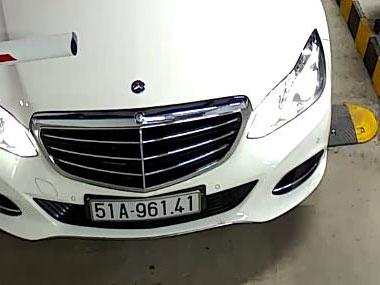
\includegraphics[width=0.75\textwidth]{images/yolo_label_example.png}
	\caption{Ví dụ ảnh biển số tượng trưng cho tập dữ liệu}
	\label{fig}
\end{figure}

\begin{table}[H]
	\centering
	\caption{Thống kê số lượng đối tượng biển số trong mỗi ảnh của bộ dữ liệu YOLO}
	\label{tab:yolo_object_per_image_total}
	\renewcommand{\arraystretch}{1.4}
	\begin{tabular}{|c|r|r|}
		\hline
		\textbf{Số biển số trong ảnh} & \textbf{Số ảnh} & \textbf{Tỷ lệ} \\
		\hline
		0 biển số & 0 & 0,00\% \\
		\hline
		1 biển số & 4.157 & 90,80\% \\
		\hline
		2 biển số & 271 & 5,92\% \\
		\hline
		Trên 2 biển số & 150 & 3,28\% \\
		\hline
		Tổng cộng & 4.578 & 100,00\% \\
		\hline
	\end{tabular}
\end{table}

Bộ dữ liệu nhiều loại ảnh 1 biển ,ảnh 2  biển và ảnh nhiều hơn 2 biển số 
Mục tiêu của tập dữ liệu này là giúp mô hình học cách phát hiện vùng biển số trong ảnh đầu vào. Sau khi huấn luyện, mô hình YOLO nhận ảnh xe và trả về vị trí biển số. Kết quả này là bước đầu vào cho giai đoạn nhận dạng ký tự. Nếu vùng biển số được phát hiện sai hoặc thiếu chính xác, chất lượng nhận dạng OCR ở bước sau cũng bị ảnh hưởng.



\subsection{Dữ liệu huấn luyện mô hình OCR}

Dữ liệu huấn luyện mô hình OCR gồm các ảnh biển số đã được cắt từ ảnh gốc và nhãn văn bản tương ứng. Mỗi ảnh trong tập OCR chứa vùng biển số, còn nhãn là chuỗi ký tự thực tế xuất hiện trên biển số đó. Ví dụ, một ảnh biển số có thể được gán nhãn dạng “30F11292” hoặc “51A12345” tùy theo nội dung biển số.

Tập dữ liệu OCR được xây dựng từ hai nguồn chính. Nguồn thứ nhất là bộ dữ liệu Vietnamese License Plate OCR trên Kaggle ~\cite{kaggle_vietnamese_plate_ocr}.Bộ dữ liệu bao gồm 11096 ảnh và nhãn biển số Xe Việt nam được chia thành 2 tệp gồm cropped và generated .Với file cropped là ảnh biển số được cắt ra nên sẽ hơi mờ và nhỏ còn file generated là ảnh biến số của cropped nhưng cực kỳ rõ nét, làm tăng độ đa dạng của dữ liệu. bộ dữ liệu Vietnamese License Plate OCR là nguồn dữ liệu chính dùng để huấn luyện mô hình nhận dạng ký tự biển số xe. 

Nguồn thứ hai là các ảnh biển số được cắt từ bộ dữ liệu phát hiện bằng mô hình YOLO. Đây là nhóm dữ liệu bổ sung, được dùng để tăng số lượng mẫu ký tự hiếm cho việc huấn luyện cho OCR. Khác với bộ dữ liệu Kaggle, các ảnh được cắt từ YOLO chưa có nhãn ký tự đi kèm, nên cần được gán nhãn thủ công trước khi đưa vào huấn luyện. Mục đích chính của nhóm dữ liệu này là bổ sung các ký tự biển số ít xuất hiện trong bộ dữ liệu chính vd :'Y' , 'U' , 'V' từ đó giảm tình trạng lệch phân bố ký tự và giúp mô hình học tốt hơn với các trường hợp hiếm.



\subsection{Phân chia dữ liệu train, validation và test mô hình YOLO}



Đối với dữ liệu để train mô hình YOLO, Sau khi hoàn tất tiền xử lý, toàn bộ 4578 mẫu được chia thành ba tập train, validation và test theo tỷ lệ 80/10/10 . kết với sự phân bỗ dữ nhiều biển số trong ảnh điều giúp kết quả đánh giá trở nên minh bạch hơn .

\begin{table}[H]
	\centering
	\caption{Kết quả chia file dữ liệu huấn luyện mô hình YOLO}
	\label{tab:ket_qua_chia_file}
	\begin{tabular}{|l|c|r|l|}
		\hline
		\textbf{Tập} & \textbf{Tỷ lệ} & \textbf{Số mẫu}  \\ 
		\hline
		Train & 80\% & 3.632 \\ 
		\hline
		Validation & 10\% & 4.72\\ 
		\hline
		Test & 10\% & 4.73 \\ 
		\hline
	\end{tabular}
\end{table}

\begin{table}[H]
	\centering
	\caption{Thống kê số lượng đối tượng biển số trong mỗi ảnh của bộ dữ liệu YOLO}
	\label{tab:yolo_object_per_image_split}
	\renewcommand{\arraystretch}{1.4}
	\begin{tabular}{|c|c|r|r|}
		\hline
		\textbf{Tập dữ liệu} & \textbf{Số biển số trong ảnh} & \textbf{Số ảnh} & \textbf{Tỷ lệ} \\
		\hline
		Train & 0 biển số & 0 & 0,00\% \\
		\hline
		Train & 1 biển số & 3.330 & 91,66\% \\
		\hline
		Train & 2 biển số & 188 & 5,17\% \\
		\hline
		Train & Trên 2 biển số & 115 & 3,17\% \\
		\hline
		\textbf{Tổng Train} &  & \textbf{3.633} & \textbf{100,00\%} \\
		\hline
		
		Validation & 0 biển số & 0 & 0,00\% \\
		\hline
		Validation & 1 biển số & 411 & 87,08\% \\
		\hline
		Validation & 2 biển số & 42 & 8,90\% \\
		\hline
		Validation & Trên 2 biển số & 19 & 4,03\% \\
		\hline
		\textbf{Tổng Validation} &  & \textbf{472} & \textbf{100,00\%} \\
		\hline
		
		Test & 0 biển số & 0 & 0,00\% \\
		\hline
		Test & 1 biển số & 416 & 87,95\% \\
		\hline
		Test & 2 biển số & 41 & 8,67\% \\
		\hline
		Test & Trên 2 biển số & 16 & 3,38\% \\
		\hline
		\textbf{Tổng Test} &  & \textbf{473} & \textbf{100,00\%} \\
		\hline
		
	\end{tabular}
\end{table}

\section{Chuẩn bị dữ liệu cho mô hình OCR}

\subsection{Làm sạch nhãn biển số}

Nhãn biển số là chuỗi ký tự dùng làm kết quả đúng khi huấn luyện mô hình OCR. Nếu nhãn sai hoặc không thống nhất, mô hình sẽ học sai quan hệ giữa ảnh và ký tự. Vì vậy, trước khi huấn luyện, toàn bộ nhãn được kiểm tra và chuẩn hóa.

Các nhãn được đưa về cùng một quy ước ghi. Khoảng trắng thừa được loại bỏ, các ký tự không hợp lệ được kiểm tra lại và các trường hợp sai định dạng được tách ra để xử lý thủ công. Với biển số xe, nhãn chỉ giữ lại các chữ số và chữ cái hợp lệ. Các dấu gạch ngang, dấu chấm hoặc ký tự đặc biệt không cần thiết được loại bỏ nếu không được dùng trong quá trình nhận dạng.

\begin{table}[H]
	\centering
	\caption{Ví dụ nhãn biển số trước và sau khi làm sạch}
	\label{tab:vi_du_lam_sach_nhan_ocr}
	\begin{tabular}{|c|c|c|}
		\hline
		\textbf{STT} & \textbf{Nhãn ban đầu} & \textbf{Nhãn sau làm sạch} \\
		\hline
		1 & \texttt{30F 11292} & \texttt{30F11292} \\
		\hline
		2 & \texttt{51A-12345} & \texttt{51A12345} \\
		\hline
		3 & \texttt{59C.45678} & \texttt{59C45678} \\
		\hline
		4 & \texttt{ 43D67890 } & \texttt{43D67890} \\
		\hline
		5 & \texttt{29a88888} & \texttt{29A88888} \\
		\hline
	\end{tabular}
\end{table}

Đối với nhóm ảnh được cắt từ dữ liệu YOLO, các ảnh chưa có nhãn ký tự sẵn. Vì vậy, nhãn được tạo thủ công dựa trên nội dung biển số trong ảnh. Sau khi gán nhãn, dữ liệu này cũng được kiểm tra theo cùng quy tắc với bộ dữ liệu chính.

\subsection{Xây dựng dictionary ký tự}

Dictionary ký tự được dùng để xác định tập ký tự mà mô hình OCR cần nhận dạng. Trong bài toán nhận dạng biển số xe, tập ký tự bao gồm : 
\begin{verbatim}
	                0 1 2 3 ... 9 A B C ... X Y Z
\end{verbatim} 

Dictionary không bao gồm ký tự đặc biệt. Những ký tự này phù hợp nhãn đã làm sạch

\subsection{Bổ sung dữ liệu ký tự hiếm}

Sau khi thống kê sự phân bố của ký tự kết quả cho thấy dữ liệu đang mất cân bằng đặc biệt với các tự ít như : R , S , U , Y , Z . vì vậy sẽ bổ sung thêm những ký tự hiếm bằng bộ dữ liệu được đọc thủ công từ trước  .

\begin{longtable}{|c|r|r|}
	\caption{So sánh phân bố ký tự trong dữ liệu OCR trước và sau khi bổ sung ký tự hiếm}
	\label{tab:char_count_compare_all} \\
	\hline
	\textbf{Ký tự} 
	& \textbf{Trước khi bổ sung ký tự hiếm} 
	& \textbf{Sau khi bổ sung ký tự hiếm} \\
	\hline
	\endfirsthead
	
	\hline
	\textbf{Ký tự} 
	& \textbf{Trước khi bổ sung ký tự hiếm} 
	& \textbf{Sau khi bổ sung ký tự hiếm} \\
	\hline
	\endhead
	
	0 & 17441 & 16973 \\
	\hline
	1 & 9235 & 9466 \\
	\hline
	2 & 7743 & 7988 \\
	\hline
	3 & 7622 & 7820 \\
	\hline
	4 & 5701 & 6037 \\
	\hline
	5 & 8381 & 9101 \\
	\hline
	6 & 8503 & 8527 \\
	\hline
	7 & 5361 & 5555 \\
	\hline
	8 & 5900 & 6062 \\
	\hline
	9 & 7366 & 8022 \\
	\hline
	A & 3700 & 3700 \\
	\hline
	B & 977 & 977 \\
	\hline
	C & 1183 & 1183 \\
	\hline
	D & 1115 & 1115 \\
	\hline
	E & 580 & 580 \\
	\hline
	F & 957 & 957 \\
	\hline
	G & 379 & 379 \\
	\hline
	H & 1541 & 1541 \\
	\hline
	K & 1045 & 1046 \\
	\hline
	L & 1138 & 1138 \\
	\hline
	M & 624 & 286 \\
	\hline
	N & 198 & 276 \\
	\hline
	P & 369 & 369 \\
	\hline
	Q & 220 & 220 \\
	\hline
	R & 55 & 100 \\
	\hline
	S & 146 & 317 \\
	\hline
	T & 560 & 560 \\
	\hline
	U & 57 & 134 \\
	\hline
	V & 191 & 287 \\
	\hline
	X & 108 & 303 \\
	\hline
	Y & 50 & 96 \\
	\hline
	Z & 59 & 119 \\
	\hline

	
\end{longtable}


\subsection{Phân chia tập train, val, test và cân bằng dữ liệu}

Sau khi hoàn thành bước làm sạch nhãn và bổ sung dữ liệu cho các ký tự hiếm, tập dữ liệu được chia thành ba phần gồm train, validation và test với tỉ lệ là 80 /10 /10 dựa trên phân bố ký tự chữ cái trong nhãn biển số.Điều này giúp các ký tự, đặc biệt là các chữ cái ít xuất hiện, có mặt đều trong cả ba tập dữ liệu. Vd như bộ dữ liệu có 100 ký tự R thì sẽ chia tập train 80 ký tự , tập  validation và test lần lượt là 10 và 10 ký tự .Việc chia dữ liệu như vậy sẽ giúp phản ánh kết quả đánh giá mô hình 1 cách chính xác nhất .

\begin{table}[H]
	\centering
	\caption{Số lượng ảnh trong các tập dữ liệu sau khi chia}
	\label{tab:split_train_val_test}
	\begin{tabular}{|c|r|r|}
		\hline
		\textbf{Tập dữ liệu} & \textbf{Số lượng ảnh} & \textbf{Tỷ lệ} \\
		\hline
		Train & 10,010 & 80\% \\
		\hline
		Val & 1,253 & 10\% \\
		\hline
		Test & 1,252 & 10\% \\
		\hline
		Tổng cộng & 12,515 & 100\% \\
		\hline
	\end{tabular}
\end{table}
Sau khi chia dữ liệu, bước cân bằng dữ liệu chỉ được thực hiện trên tập train. Tập val và tập test được giữ nguyên để kết quả đánh giá không bị ảnh hưởng bởi dữ liệu sinh thêm.

Quá trình cân bằng tập train tập trung vào các ký tự chữ cái có tần suất thấp. Các ký tự số không được tác động vì số lượng chữ số trong biển số thường nhiều và phân bố ổn định hơn. Với các ký tự ít xuất hiện như R, U, Y hoặc Z, dữ liệu được tăng cường bằng các kỹ thuật biến đổi ảnh. Các biến đổi được dùng gồm thay đổi độ sáng, thay đổi độ tương phản, đổi sắc độ màu, làm mờ nhẹ, thêm nhiễu nhẹ và biến đổi nhỏ về hình học. Những kỹ thuật này giúp tạo thêm các mẫu huấn luyện khác nhau từ ảnh gốc, nhưng vẫn giữ nguyên nội dung nhãn biển số.

\begin{figure}[h]
	\centering
	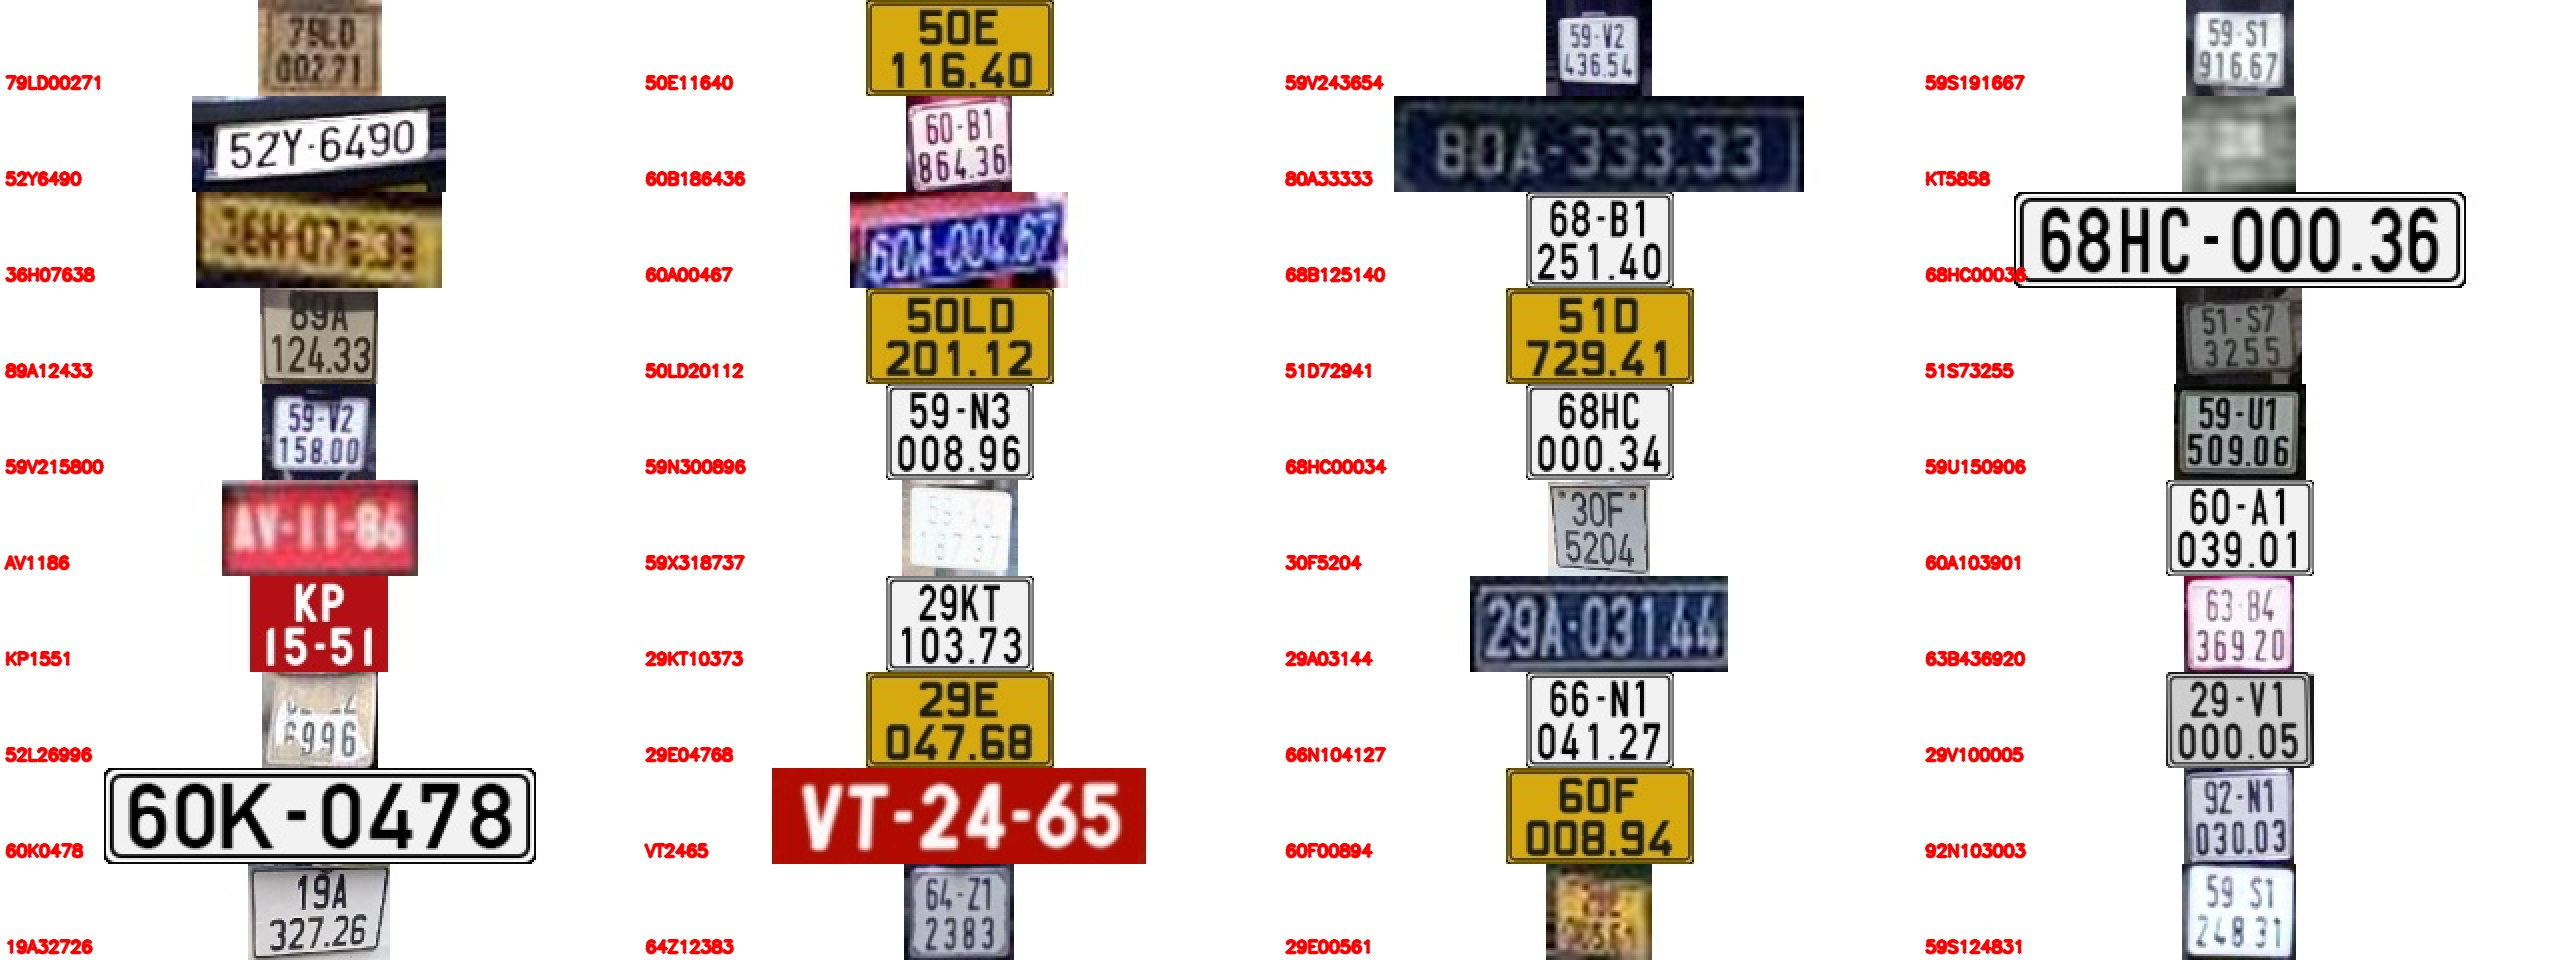
\includegraphics[width=0.85\textwidth]{images/lam_giau_anh.jpg}
	\caption{Một số biển số ký hiếm được tạo thêm vào }
	\label{fig:augmentation_example}
\end{figure}

Đối với các ký tự xuất hiện quá nhiều, tập train được giảm bớt một phần mẫu liên quan đến các chữ cái phổ biến. Mục tiêu là giảm thiểu độ chênh lệch và tránh để mô hình thiên về những ký tự xuất hiện nhiều trong quá trình học. Việc giảm mẫu không áp dụng cho ký tự số .
\begin{longtable}{|c|r|c|r|c|r|}
	\caption{Tần suất ký tự trong tập train sau khi cân bằng dữ liệu}
	\label{tab:char_frequency_train_balanced} \\
	\hline
	\textbf{Ký tự} & \textbf{Số lần} 
	& \textbf{Ký tự} & \textbf{Số lần} 
	& \textbf{Ký tự} & \textbf{Số lần} \\
	\hline
	\endfirsthead
	
	\hline
	\textbf{Ký tự} & \textbf{Số lần} 
	& \textbf{Ký tự} & \textbf{Số lần} 
	& \textbf{Ký tự} & \textbf{Số lần} \\
	\hline
	\endhead
	
	0 & 7910 & 5 & 7006 & 1 & 6611 \\
	\hline
	9 & 5960 & 2 & 5616 & 3 & 5387 \\
	\hline
	6 & 5315 & 4 & 4595 & 8 & 4305 \\
	\hline
	7 & 4192 & A & 1899 & K & 691 \\
	\hline
	H & 690 & L & 561 & B & 545 \\
	\hline
	D & 521 & S & 500 & X & 500 \\
	\hline
	V & 500 & N & 500 & C & 478 \\
	\hline
	F & 470 & T & 395 & P & 266 \\
	\hline
	E & 263 & R & 250 & U & 250 \\
	\hline
	Y & 250 & Z & 250 & G & 199 \\
	\hline
	M & 182 &  &  &  &  \\
	\hline

	
\end{longtable}

Sau khi hoàn tất bước cân bằng dữ liệu, toàn bộ ảnh trong tập train được chuẩn hóa về cùng kích thước 48$\times$320 bằng phương pháp resize kết hợp padding.Cách làm này giúp ảnh có kích thước thống nhất nhưng vẫn giữ được tỷ lệ gốc của biển số, hạn chế tình trạng ký tự bị kéo giãn hoặc bị mất ở mép ảnh. Nhờ đó, cả ảnh gốc và ảnh sinh thêm đều có cùng định dạng trước khi đưa vào huấn luyện PaddleOCR .

\begin{figure}[H]
	\centering
	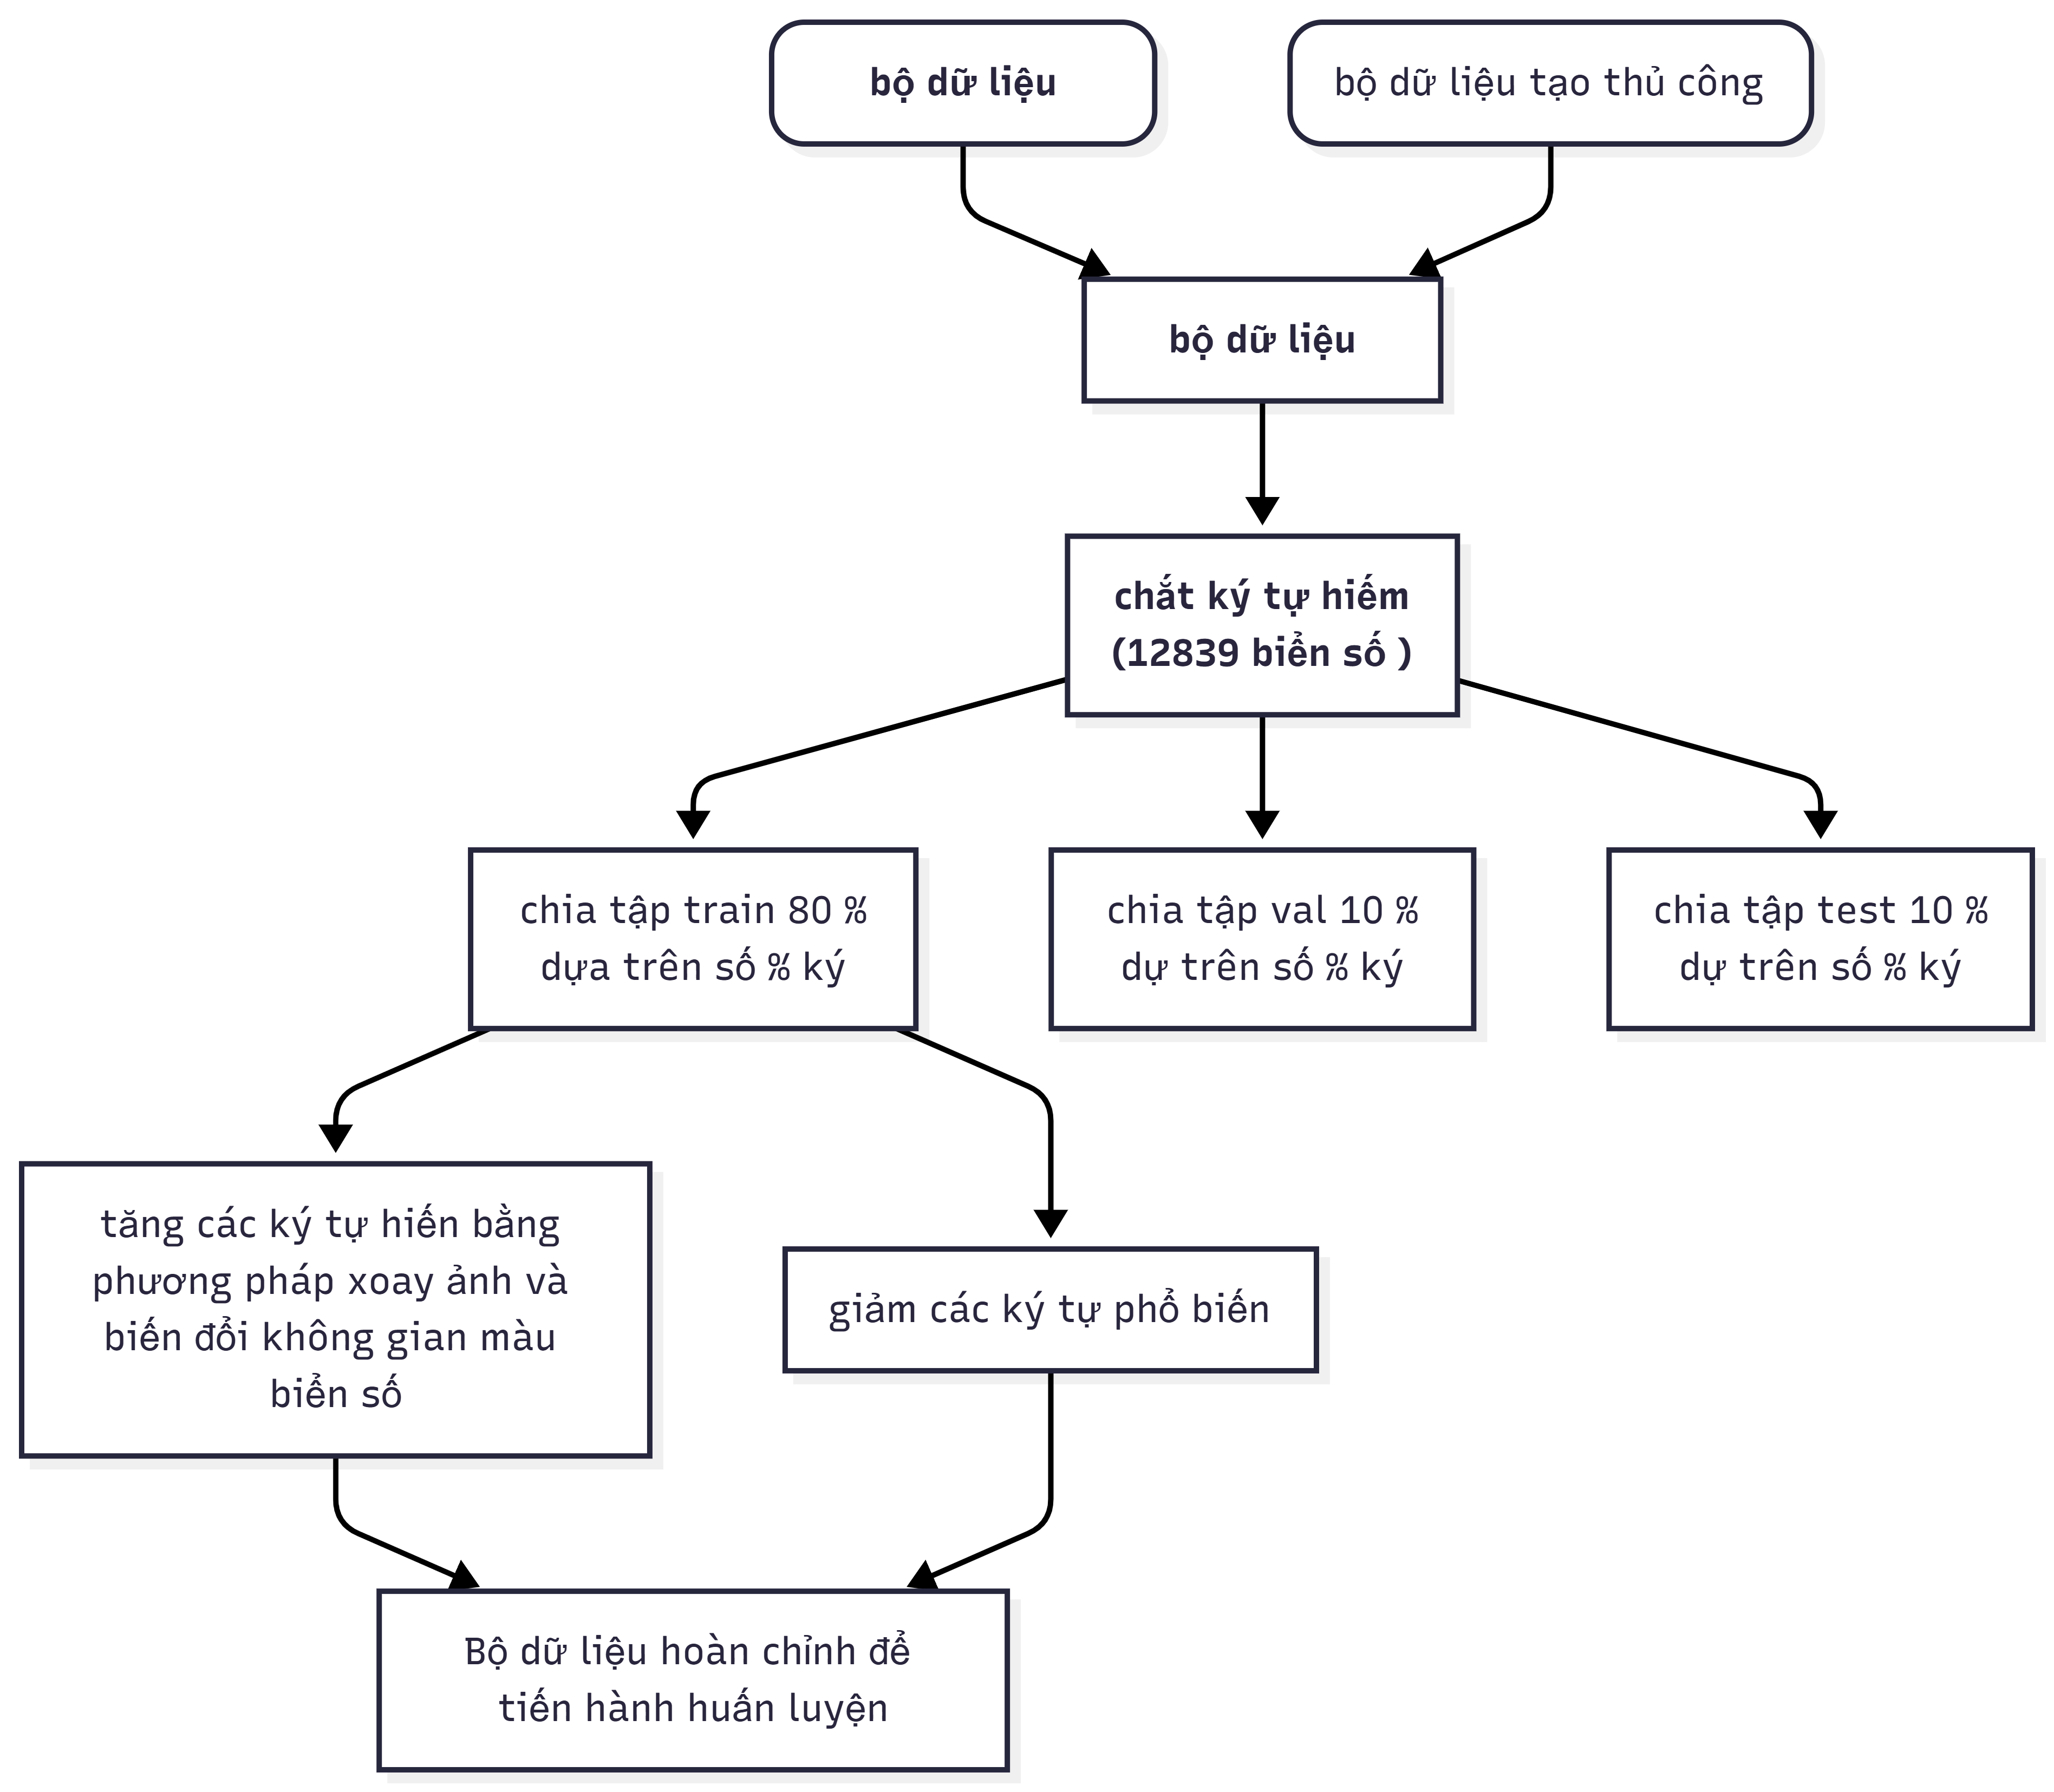
\includegraphics[width=0.9\textwidth]{images/quy_trinh_chuan_hoa_train_ocr.png}
	\caption{Tổng quy trình xử lý dữ liệu OCR}
	\label{fig:ocr_train_balance_resize_padding}
\end{figure}



\section{Huấn luyện và đánh giá mô hình YOLO}


\subsection{Vai trò của huấn luyện YOLO trong hệ thống}



Trong hệ thống nhận dạng biển số xe, YOLO đảm nhận vai trò \textbf{phát hiện vị trí biển số} bước đầu tiên và quan trọng nhất trong toàn bộ pipeline xử lý. 

% =====================================================================
% CHỖ CHÈN ẢNH: Sơ đồ vị trí YOLO trong pipeline nhận dạng biển số
% =====================================================================
\begin{figure}[H]
	\centering
	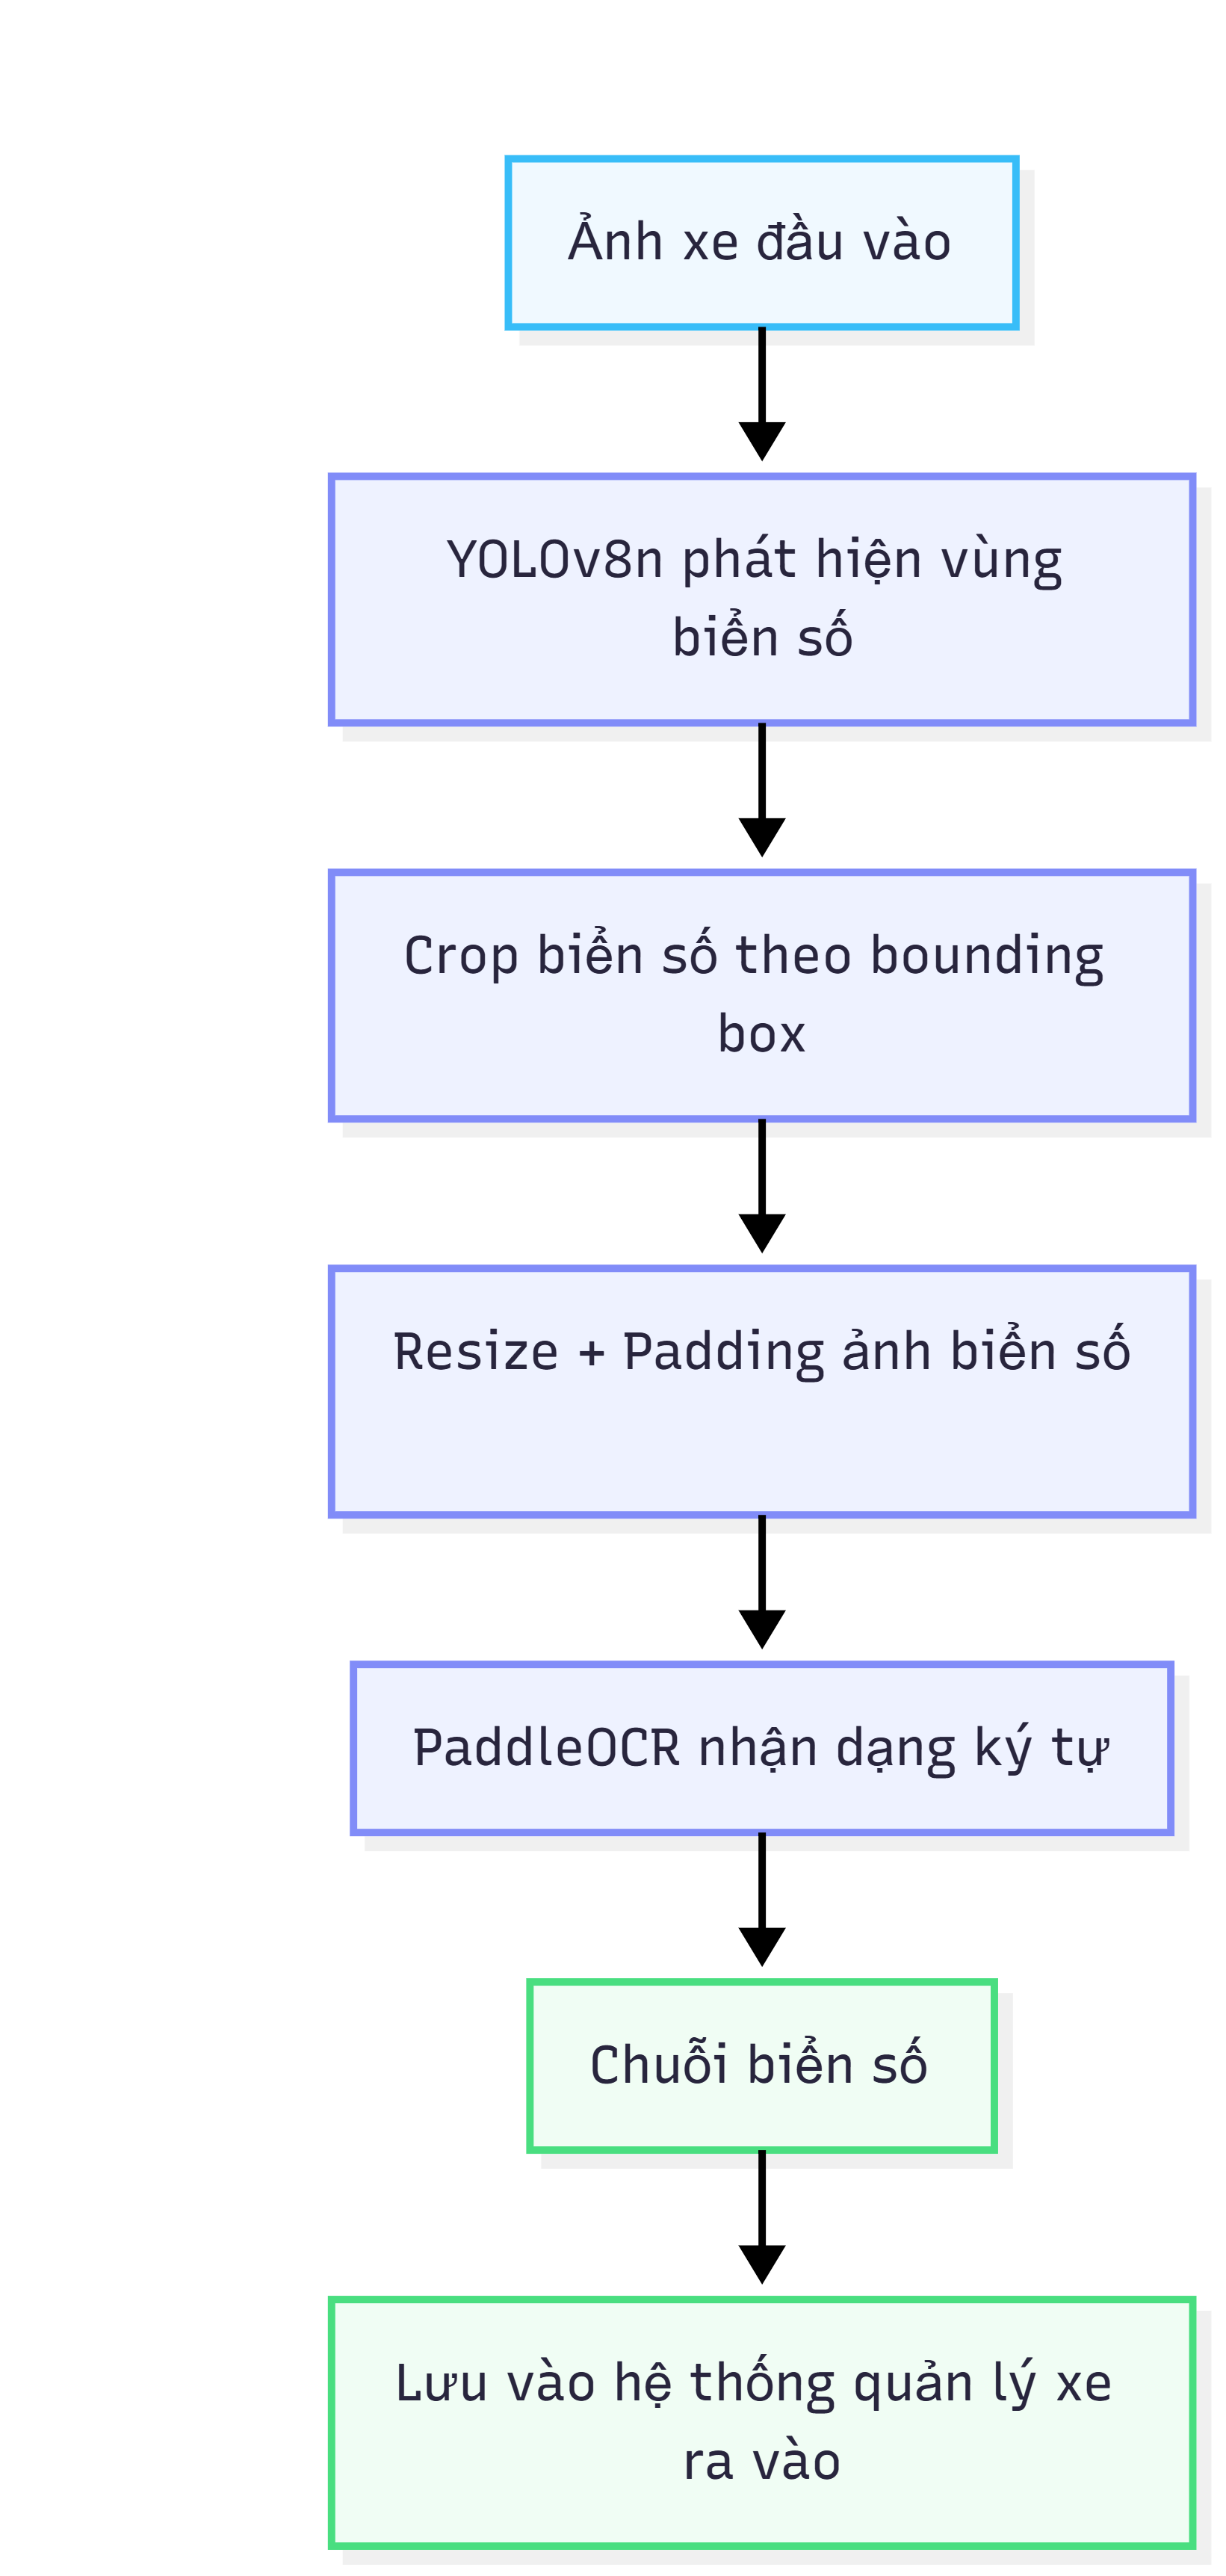
\includegraphics[width=0.35\textwidth]{images/yolo_to_ocr_pipeline.png}
	\caption{Vị trí của mô hình YOLO trong pipeline nhận dạng biển số xe.}
	\label{fig:yolo_pipeline}
\end{figure}
% =====================================================================

Ảnh xe đầu vào trước tiên được đưa vào mô hình YOLOv8n để phát hiện vùng biển số. Kết quả của bước này là bounding box bao quanh biển số trong ảnh. Từ bounding box đó, hệ thống crop vùng biển số ra khỏi ảnh gốc để tạo ảnh đầu vào cho mô hình OCR.

Sau khi crop, ảnh biển số được chuẩn hóa bằng resize kết hợp padding. Bước này giúp ảnh có kích thước thống nhất, đồng thời hạn chế việc làm méo ký tự trên biển số. Ảnh đã chuẩn hóa được đưa vào PaddleOCR để nhận dạng chuỗi ký tự. Kết quả đầu ra là chuỗi biển số, sau đó được lưu vào hệ thống quản lý xe ra vào.

Trong quy trình này, YOLO giữ vai trò là bước phát hiện đầu tiên. Nếu YOLO phát hiện sai vị trí biển số, crop thiếu ký tự hoặc bỏ sót biển số, mô hình OCR phía sau sẽ khó nhận dạng chính xác. 





% =====================================================================
% CHỖ CHÈN ẢNH: Kết quả nhận diện biển số bằng YOLO (ảnh thực tế)
% =====================================================================
\begin{figure}[H]
	\centering
	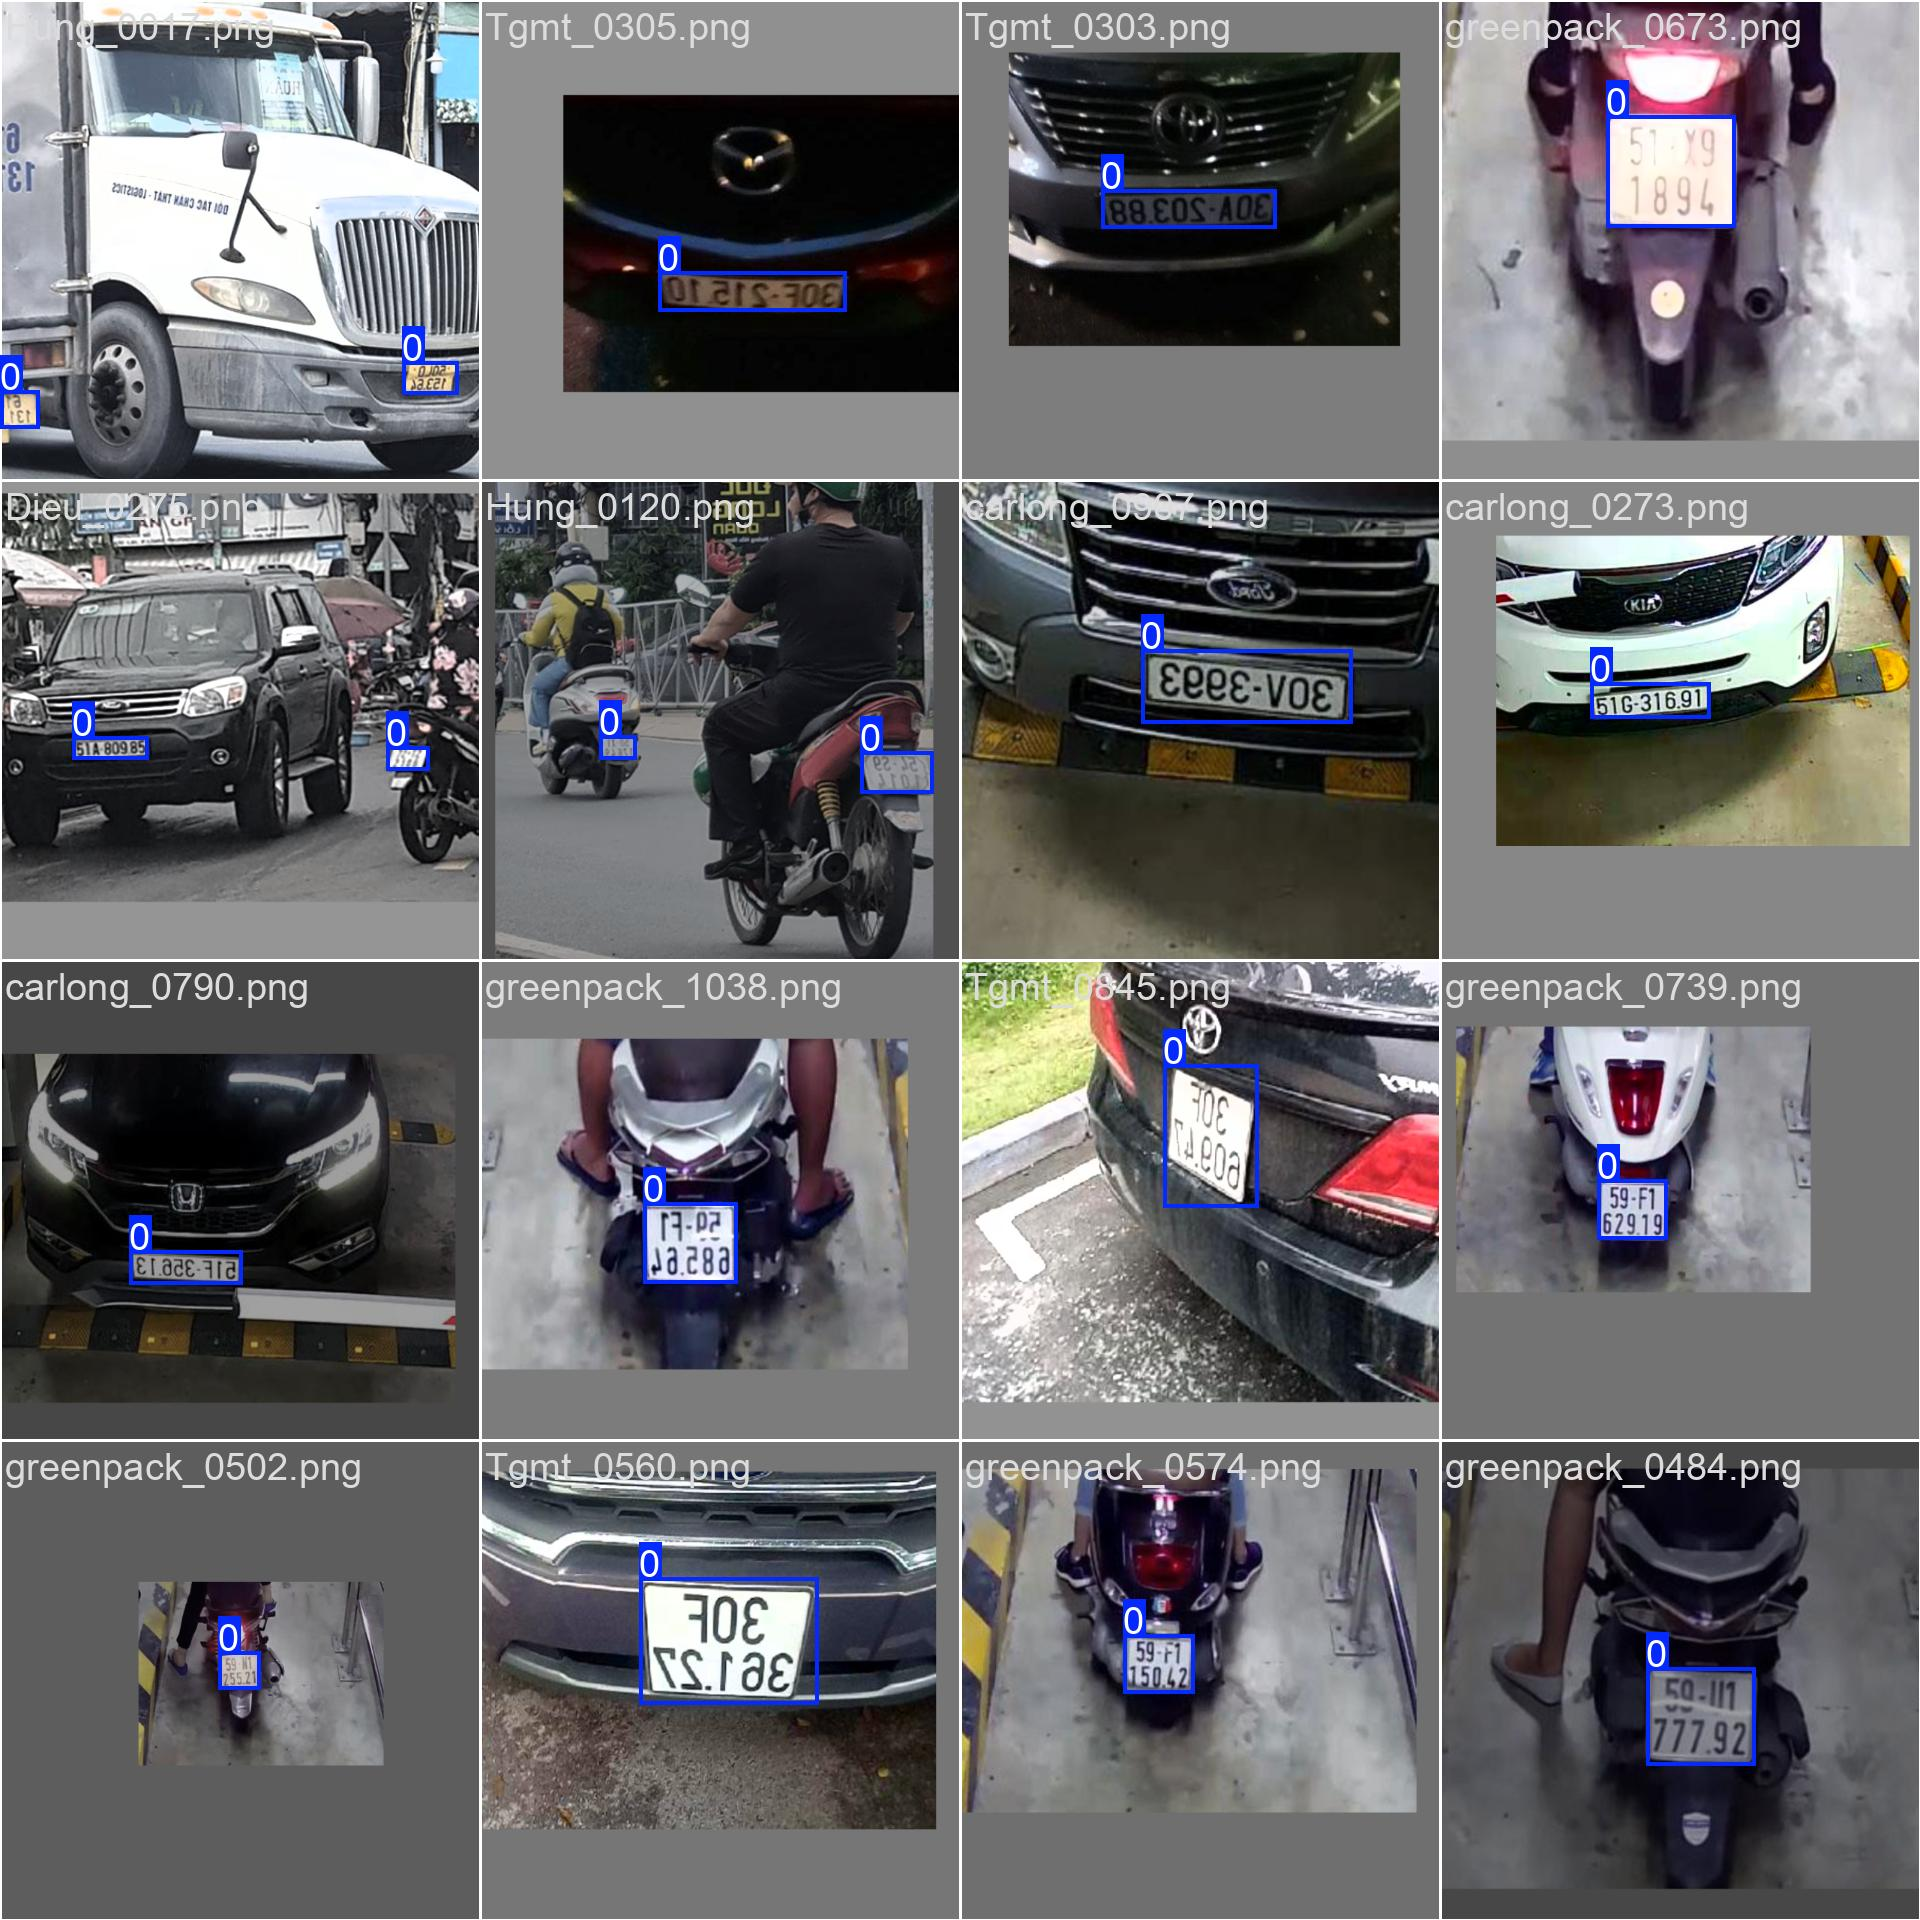
\includegraphics[width=0.9\textwidth]{images/yolo_detect_examples.jpg}
	\caption{Kết quả phát hiện biển số xe bằng mô hình YOLOv8 với hộp giới hạn.}
	\label{fig:yolo_result}
\end{figure}
% =====================================================================
Một số kết quả mà mô hình đọc được trong biển số ,mô hình cho thấy có khả năng phát hiện chính xác vùng biển số trong nhiều điều kiện ánh sáng và góc chụp khác nhau, tạo tiền đề thuận lợi cho các bước xử lý tiếp theo trong hệ thống.


\subsection{Cấu hình huấn luyện YOLOv8n}

Mô hình YOLOv8n được sử dụng trong đề tài để phát hiện vùng biển số xe trong ảnh đầu vào.Quá trình huấn luyện được thực hiện bằng thư viện Ultralytics với mô hình nền \texttt{yolov8n.pt}. Mô hình sử dụng trọng số pretrained, sau đó được huấn luyện lại trên dữ liệu biển số của đề tài. Các thông số chính gồm số epoch tối đa là 100, batch size là 16, kích thước ảnh đầu vào là 640 và cơ chế dừng sớm với patience bằng 20. 

\begin{table}[H]
	\centering
	\caption{Cấu hình huấn luyện mô hình YOLOv8n trên Google Colab}
	\label{tab:yolo_train_config_colab}
	\renewcommand{\arraystretch}{1.4}
	\begin{tabular}{|p{5cm}|p{8cm}|}
		\hline
		\textbf{Thông số} & \textbf{Giá trị} \\
		\hline
		Mô hình & YOLOv8n \\
		\hline
		Framework & Ultralytics \\
		\hline
		Task & Detect \\
		\hline
		Số lớp đối tượng & 1 lớp, biển số xe \\
		\hline
		Tổng số ảnh & 4.577 ảnh \\
		\hline
		Train / Validation / Test & 3.632 / 472 / 473  \\
		\hline
		Số ảnh validation khi huấn luyện & 472 ảnh \\
		\hline
		Số đối tượng validation & 560 biển số \\
		\hline
		Epoch & 100 \\
		\hline
		Patience & 20 \\
		\hline
		Batch size & 16 \\
		\hline
		Image size & 640 \\
		\hline
		Pretrained model & \texttt{yolov8n.pt} \\
		\hline
		Thiết bị huấn luyện & Google Colab GPU \\
		\hline
	\end{tabular}
\end{table}



\subsection{Kết quả đánh giá mô hình YOLO}

\begin{figure}[H]
	\centering
	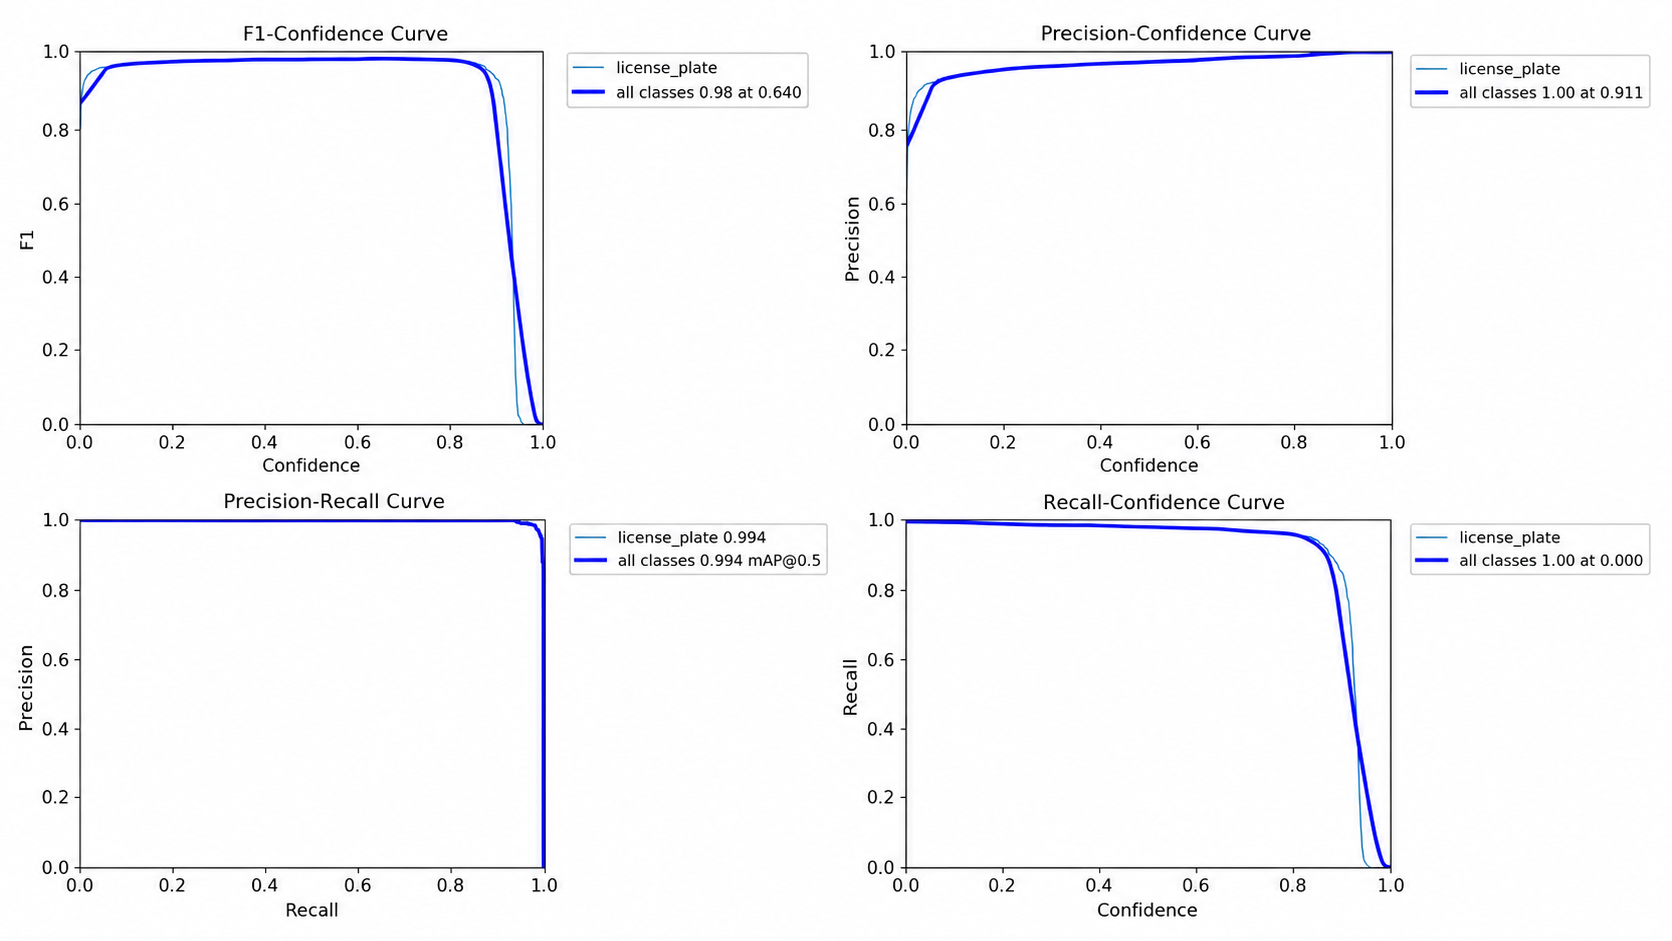
\includegraphics[width=1.1\textwidth]{images/bieudo1.png}
	\caption{Các đường cong đánh giá mô hình YOLOv8n}
	\label{fig:yolo_training_process}
\end{figure}
Đường cong F1-Confidence cho thấy F1 đạt giá trị cao nhất khoảng 0,98 tại ngưỡng confidence gần 0,64. Đây là vùng ngưỡng có sự cân bằng tốt giữa Precision và Recall. 

Đường cong Precision-Confidence cho thấy khi ngưỡng confidence tăng, Precision của mô hình cũng tăng và đạt gần 1,0 ở vùng ngưỡng cao.Cho thấy các dự đoán có độ tin cậy cao thường là các dự đoán đúng.

Đường cong Precision-Recall nằm sát vùng góc trên bên phải và có giá trị mAP@0.5 khoảng 0,994.Mô hình có khả năng duy trì Precision cao trong khi Recall vẫn lớn.

Đường cong Recall-Confidence cho thấy Recall giữ ở mức cao khi ngưỡng confidence thấp và trung bình, sau đó giảm mạnh khi confidence tiến gần 1,0. Đây là hiện tượng thường gặp trong phát hiện đối tượng. Khi đặt ngưỡng confidence quá cao, mô hình chỉ giữ lại các dự đoán chắc chắn nhất, nhưng đồng thời loại bỏ một số biển số đúng có độ tin cậy thấp hơn.



\begin{figure}[H]
	\centering
	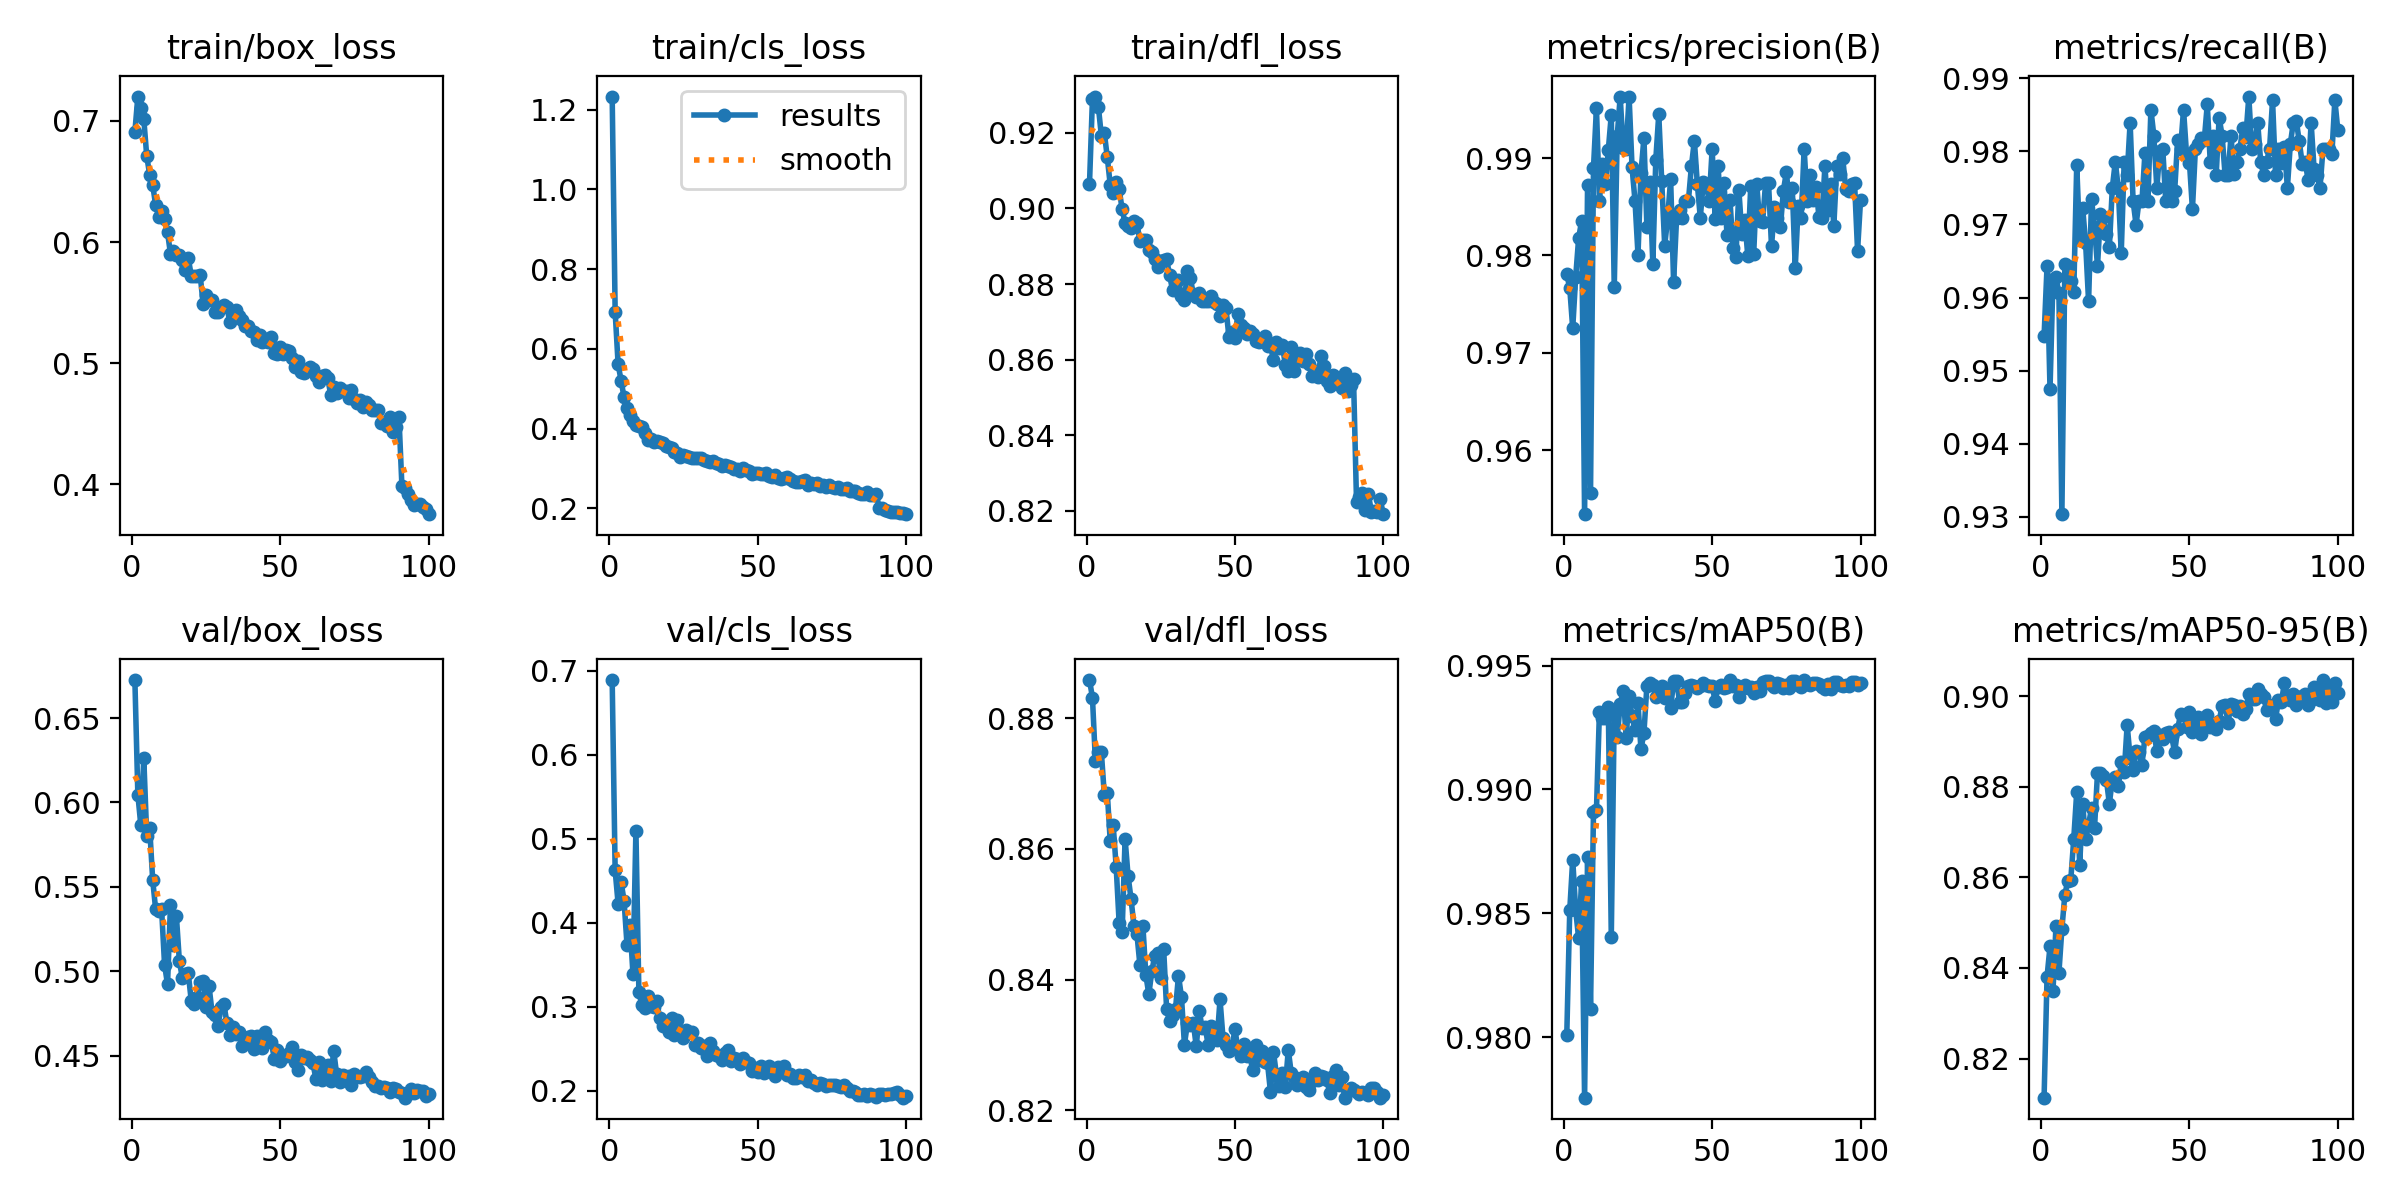
\includegraphics[width=1.0\textwidth]{images/results.png}
	\caption{Biểu đồ loss và các chỉ số trong quá trình huấn luyện}
	\label{fig:yolo_training_process}
\end{figure}

Các biểu đồ đường cong loss và chỉ số đánh giá trong quá trình huấn luyện mô hình YOLOv8n qua 100 epoch.
Cụ thể
\texttt{train/box\_loss} giảm từ 0,71 xuống 0,38 và 
\texttt{val/box\_loss} giảm từ 0,67 xuống 0,43, phản ánh khả năng định vị 
bounding box được cải thiện liên tục trên cả hai tập dữ liệu. 
\texttt{train/cls\_loss} và \texttt{val/cls\_loss} giảm nhanh trong các epoch 
đầu và ổn định quanh mức 0,20 ở cuối quá trình — kết quả phù hợp với bài toán đơn lớp. Thành phần \texttt{dfl\_loss} cũng giảm dần, cho thấy chất lượng tinh chỉnh hộp giới hạn được cải thiện theo từng epoch.

Về các chỉ số đánh giá, Precision duy trì trên 0,98 và Recall tăng dần đạt khoảng 0,98 ở cuối quá trình huấn luyện. Chỉ số mAP@0.5 đạt gần 0,995, trong khi mAP@0.5:0.95 tăng từ 0,81 lên 0,90, cho thấy mô hình không chỉ phát hiện chính xác biển số mà còn đảm bảo chất lượng định vị ở các ngưỡng IoU khắt khe.
\begin{table}[H]
	\centering
	\caption{Kết quả đánh giá mô hình YOLOv8n trên tập test}
	\label{tab:yolo_test_results}
	\renewcommand{\arraystretch}{1.4}
	\begin{tabular}{|p{5cm}|p{5cm}|}
		\hline
		\textbf{Chỉ số} & \textbf{Giá trị} \\
		\hline
		Số ảnh test & 473 ảnh \\
		\hline
		Số đối tượng biển số & 553 biển số \\
		\hline
		Precision & 0,9558 \\
		\hline
		Recall & 0,8608 \\
		\hline
		mAP50 & 0,8610 \\
		\hline
		mAP50-95 & 0,7689 \\
		\hline
		Thời gian tiền xử lý & 1,0 ms/ảnh \\
		\hline
		Thời gian suy luận & 44,0 ms/ảnh \\
		\hline
		Thời gian hậu xử lý & 0,3 ms/ảnh \\
		\hline
	\end{tabular}
\end{table}
trình bày kết quả đánh giá mô hình YOLOv8n trên tập 
test gồm 473 ảnh với tổng cộng 553 đối tượng biển số. Mô hình đạt Precision 
0,9558 và Recall 0,8608, cho thấy tỉ lệ phát hiện đúng cao trong khi vẫn còn 
bỏ sót một số biển số. Chỉ số mAP@0.5 đạt 0,8610 và mAP@0.5:0.95 đạt 0,7689, 
phản ánh chất lượng định vị chấp nhận được ở ngưỡng IoU tiêu chuẩn nhưng còn 
hạn chế khi đánh giá ở các ngưỡng IoU khắt khe hơn. Về tốc độ xử lý, tổng 
thời gian suy luận là 44,0~ms/ảnh, đáp ứng yêu cầu xử lý gần thời gian thực 
trong điều kiện thực tế.

\begin{figure}[H]
	\centering
	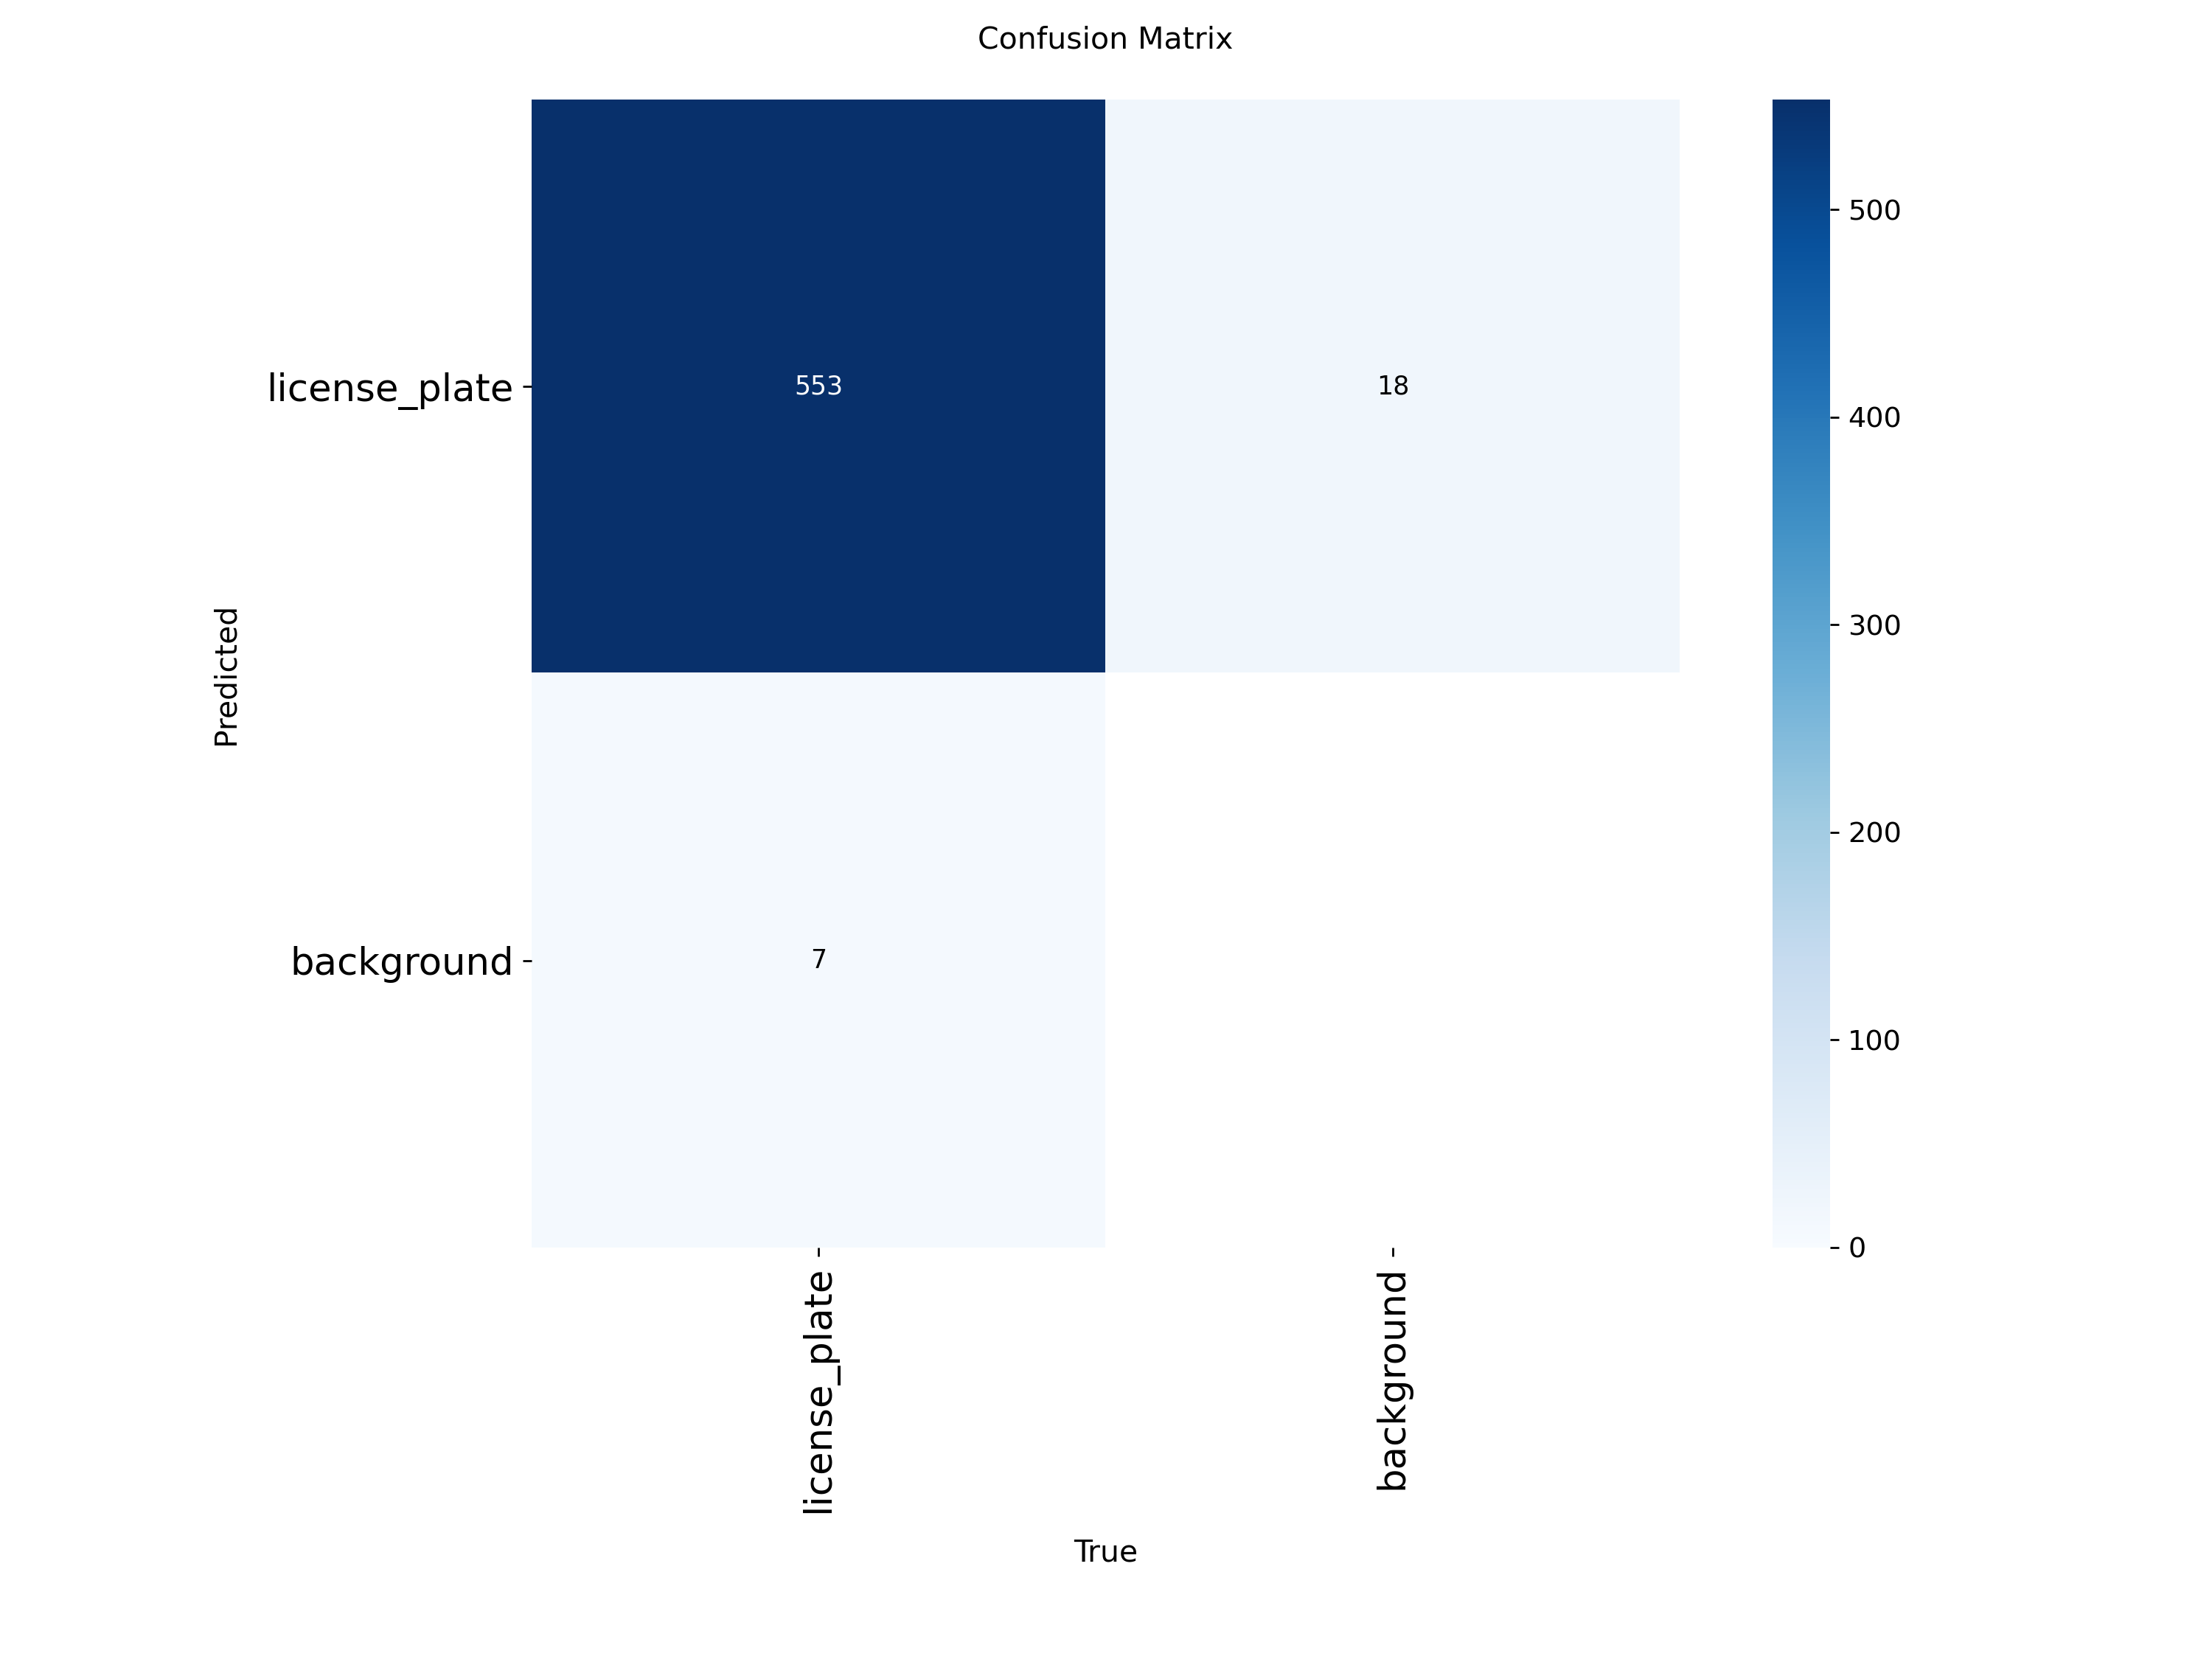
\includegraphics[width=1.0\textwidth]{images/confusion_matrix.png}
	\caption{Ma trận nhầm lẫn trên tập test}
	\label{fig:confusion_matrix}
\end{figure}


Ma trận nhầm lẫn cung cấp thêm thông tin 
chi tiết về hành vi phân loại của mô hình. Trong tổng số 553 biển số thực tế, 
mô hình phát hiện đúng 553 trường hợp (True Positive), bỏ sót 18 biển số do 
phân loại nhầm thành nền (False Negative), và nhận diện nhầm 7 vùng nền thành 
biển số (False Positive). Sự mất cân đối giữa False Negative (18) và False 
Positive (7) cho thấy mô hình có xu hướng thận trọng — ưu tiên độ chính xác 
hơn độ bao phủ — điều này phù hợp với giá trị Precision cao hơn Recall quan 
sát được ở Bảng~\ref{tab:yolo_test_results}.

Theo cái nhìn tổng quát, mô hình YOLOv8n đã được huấn luyện thành công và cho thấy khả 
năng phát hiện biển số xe đáng tin cậy. Mô hình hội tụ ổn định trong quá 
trình huấn luyện, đạt độ chính xác cao trên tập test và duy trì tốc độ xử lý 
phù hợp với yêu cầu thời gian thực. Kết quả này khẳng định YOLOv8n là lựa 
chọn phù hợp cho giai đoạn phát hiện biển số trong hệ thống, tạo tiền đề 
thuận lợi cho bước nhận dạng ký tự ở các giai đoạn tiếp theo.


\section{Huấn luyện và đánh giá mô hình Paddle OCR}

\subsection{Cấu hình huấn luyện}

Mô hình OCR trong đề tài được huấn luyện bằng framework PaddleOCR .Cấu hình nhận dạng sử dụng hướng tiếp cận của PP-OCRv4 Recognition, với kiến trúc nhận dạng \texttt{SVTR\_LCNet}.Quá trình huấn luyện được thực hiện trên Google Colab với GPU nhằm rút ngắn thời gian xử lý. Mô hình sử dụng cấu hình nhận dạng của PaddleOCR, hàm mất mát CTC kết hợp NRTR và batch size 64 ,Số epoch huấn luyện là 50. Trong quá trình huấn luyện, mô hình được đánh giá định kỳ trên tập validation bằng các chỉ số Accuracy và Normalized Edit Distance.

\begin{table}[H]
	\centering
	\caption{Cấu hình huấn luyện mô hình OCR}
	\label{tab:ocr_train_config}
	\renewcommand{\arraystretch}{1.4}
	\begin{tabular}{|p{5cm}|p{8cm}|}
		\hline
		\textbf{Thông số} & \textbf{Giá trị} \\
		\hline
		Framework & PaddleOCR \\
		\hline
		Phiên bản cấu hình mô hình & PP-OCRv4 Recognition \\
		\hline
		Nhiệm vụ & Nhận dạng ký tự biển số \\
		\hline
		Dữ liệu đầu vào & Ảnh biển số đã crop \\
		\hline
		Kích thước ảnh & 48$\times$320 \\
		\hline
		Dictionary & 0-9 và A-Z \\
		\hline
		Số tập dữ liệu & Train, validation, test \\
		\hline
		Batch size & 64 \\
		\hline
		Epoch & 50 \\
		\hline
		Learning rate & 0.0005 \\
		\hline
		Hàm mất mát & CTCLoss và NRTRLoss \\
		\hline
		Thiết bị huấn luyện & Google Colab GPU \\
		\hline
	\end{tabular}
\end{table}



\subsection{Kết quả huấn luyện}



\begin{table}[H]
	\centering
	\caption{Kết quả huấn luyện mô hình Paddle OCR qua một số epoch}
	\label{tab:ocr_train_results}
	\renewcommand{\arraystretch}{1.4}
	\begin{tabular}{|c|c|c|c|c|}
		\hline
		\textbf{Epoch} & \textbf{Accuracy} & \textbf{Norm Edit Dis} & \textbf{CTC Loss} & \textbf{NRTR Loss} \\
		\hline
		1 & 0,0000 & 0,1878 & 81,3232 & 2,6452 \\
		\hline
		10 & 0,6328 & 0,9099 & 2,9994 & 0,7907 \\
		\hline
		20 & 0,8281 & 0,9594 & 1,2706 & 0,7413 \\
		\hline
		30 & 0,8750 & 0,9752 & 0,7251 & 0,7143 \\
		\hline
		42 & 0,9141 & 0,9848 & 0,3979 & 0,7035 \\
		\hline
		50 & 0,9453 & 0,9891 & 0,2902 & 0,7014 \\
		\hline
	\end{tabular}
\end{table}

\begin{figure}[H]
	\centering
	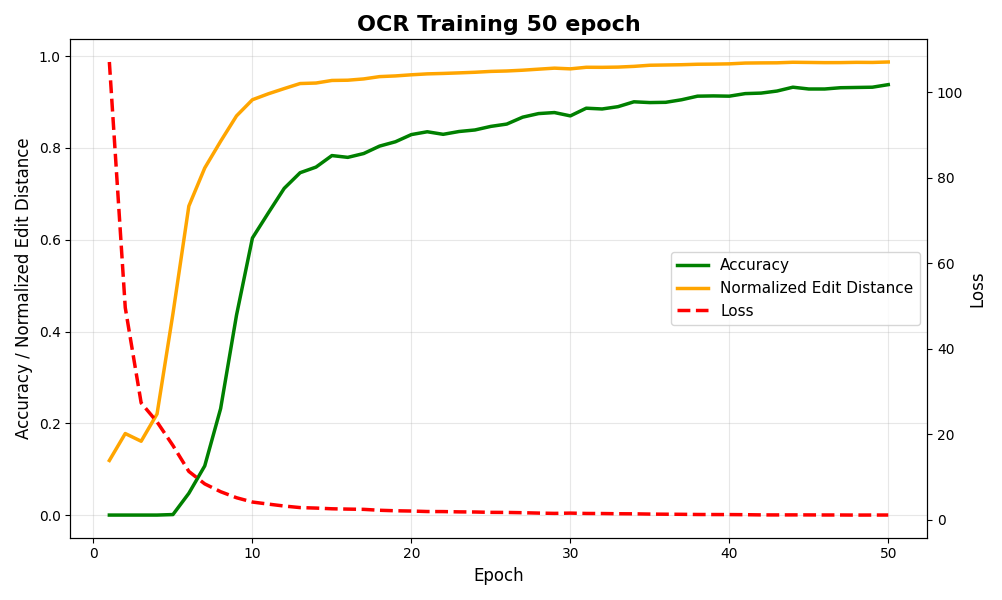
\includegraphics[width=0.9\textwidth]{images/Figure_1.png}
	\caption{Biểu đồ Accuracy, Normalized Edit Distance và Loss trong quá trình huấn luyện OCR}
	\label{fig:ocr_training_curve}
\end{figure}
Bảng~\ref{tab:ocr_train_results} và Hình~\ref{fig:ocr_training_curve} cho thấy mô hình Paddle OCR 
hội tụ nhanh và ổn định trong 50 epoch huấn luyện. CTC Loss giảm mạnh từ 
81,33 xuống 0,29, Accuracy tăng từ 0 lên 0,9453 và Normalized Edit Distance 
đạt 0,9891, phản ánh khả năng nhận dạng chuỗi ký tự biển số ngày càng chính 
xác. Đáng chú ý, phần lớn sự cải thiện diễn ra trước epoch 20, sau đó mô hình 
tiếp tục tinh chỉnh chậm và ổn định đến cuối quá trình, không có dấu hiệu 
quá khớp.


\subsection{Đánh giá trên tập validation và test}

\begin{figure}[H]
	\centering
	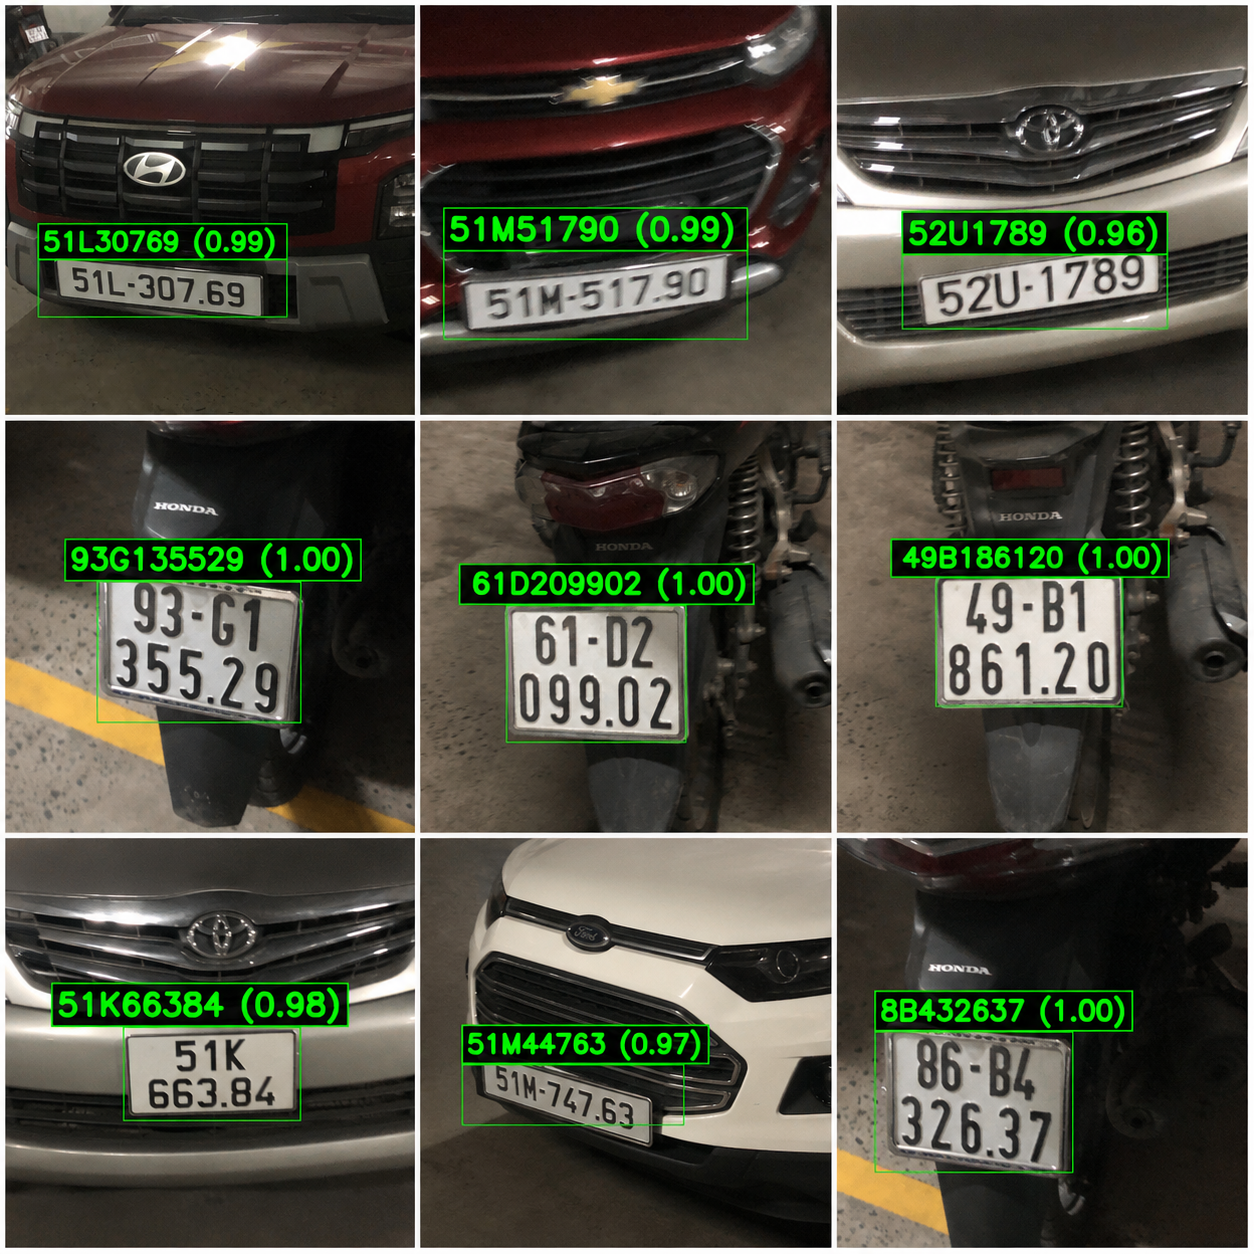
\includegraphics[width=0.9\textwidth]{images/ocr_prediction_examples.png}
	\caption{Một số kết quả nhận dạng biển số trên tập test của mô hình Paddle OCR}
	\label{fig:ocr_prediction_examples}
\end{figure}

\begin{table}[H]
	\centering
	\caption{Kết quả đánh giá mô hình OCR trên tập validation và test}
	\label{tab:ocr_eval_results}
	\renewcommand{\arraystretch}{1.4}
	\begin{tabular}{|p{4cm}|c|c|c|}
		\hline
		\textbf{Tập dữ liệu} & \textbf{Số mẫu} & \textbf{Accuracy} & \textbf{Normalized Edit Distance} \\
		\hline
		Validation & 1253 & 0,856 & 0,960 \\
		\hline
		Test & 1252 & 0,856 & 0,952 \\
		\hline
	\end{tabular}
\end{table}



Bảng~\ref{tab:ocr_eval_results} trình bày kết quả đánh giá mô hình OCR trên tập 
validation và test, mỗi tập gồm hơn 1250 mẫu. Mô hình đạt Accuracy 0,856 
và Normalized Edit Distance 0,960 trên tập validation, và duy trì kết quả 
tương đương trên tập test với Accuracy 0,856 và Normalized Edit Distance 
0,952. Sự nhất quán giữa hai tập dữ liệu cho thấy mô hình có khả năng tổng 
quát hóa tốt, không bị phụ thuộc vào dữ liệu huấn luyện. Tuy nhiên, so với 
Accuracy 0,9453 và Normalized Edit Distance 0,9891 đạt được ở epoch cuối 
trong quá trình huấn luyện, các chỉ số trên tập test giảm đáng kể, cho thấy 
vẫn còn khoảng cách giữa dữ liệu huấn luyện và dữ liệu thực tế — có thể do 
sự đa dạng về font chữ, điều kiện chụp, hoặc chất lượng ảnh đầu vào chưa 
được bao phủ đầy đủ trong tập huấn luyện. Kết hợp với quá trình huấn luyện 
hội tụ ổn định đã trình bày ở trên, có thể kết luận mô hình OCR đáp ứng yêu 
cầu cơ bản nhận dạng ký tự biển số, song cần bổ sung thêm dữ liệu đa dạng để 
thu hẹp khoảng cách này.



\subsection{Phân tích lỗi và điều chỉnh dữ liệu}

Để xác định nguyên nhân làm giảm độ chính xác của mô hình OCR, đề tài tiến hành phân tích lỗi theo từng ký tự trên tập test. Phân tích này giúp xác định ký tự nào bị nhận dạng sai nhiều và ký tự đó thường bị nhầm với ký tự nào. Đây là cơ sở để điều chỉnh lại dữ liệu huấn luyện.



\begin{table}[H]
	\centering
	\caption{Thống kê một số ký tự nhận dạng sai nhiều trên tập test}
	\label{tab:ocr_wrong_char_summary}
	\renewcommand{\arraystretch}{1.4}
	\begin{tabular}{|c|r|r|r|}
		\hline
		\textbf{Ký tự} & \textbf{Số lần xuất hiện} & \textbf{Số lần sai} & \textbf{Tỷ lệ lỗi} \\
		\hline
		3 & 778 & 39 & 5,01\% \\
		\hline
		8 & 601 & 38 & 6,32\% \\
		\hline
		0 & 1704 & 35 & 2,05\% \\
		\hline
		5 & 866 & 31 & 3,58\% \\
		\hline
		2 & 777 & 25 & 3,22\% \\
		\hline
		4 & 626 & 15 & 2,40\% \\
		\hline
		A & 404 & 10 & 2,48\% \\
		\hline
		K & 98 & 5 & 5,10\% \\
		\hline
		B & 93 & 5 & 5,38\% \\
		\hline
		L & 131 & 4 & 3,05\% \\
		\hline
		H & 152 & 4 & 2,63\% \\
		\hline
		P & 32 & 3 & 9,38\% \\
		\hline
	\end{tabular}
\end{table}

\begin{figure}[H]
	\centering
	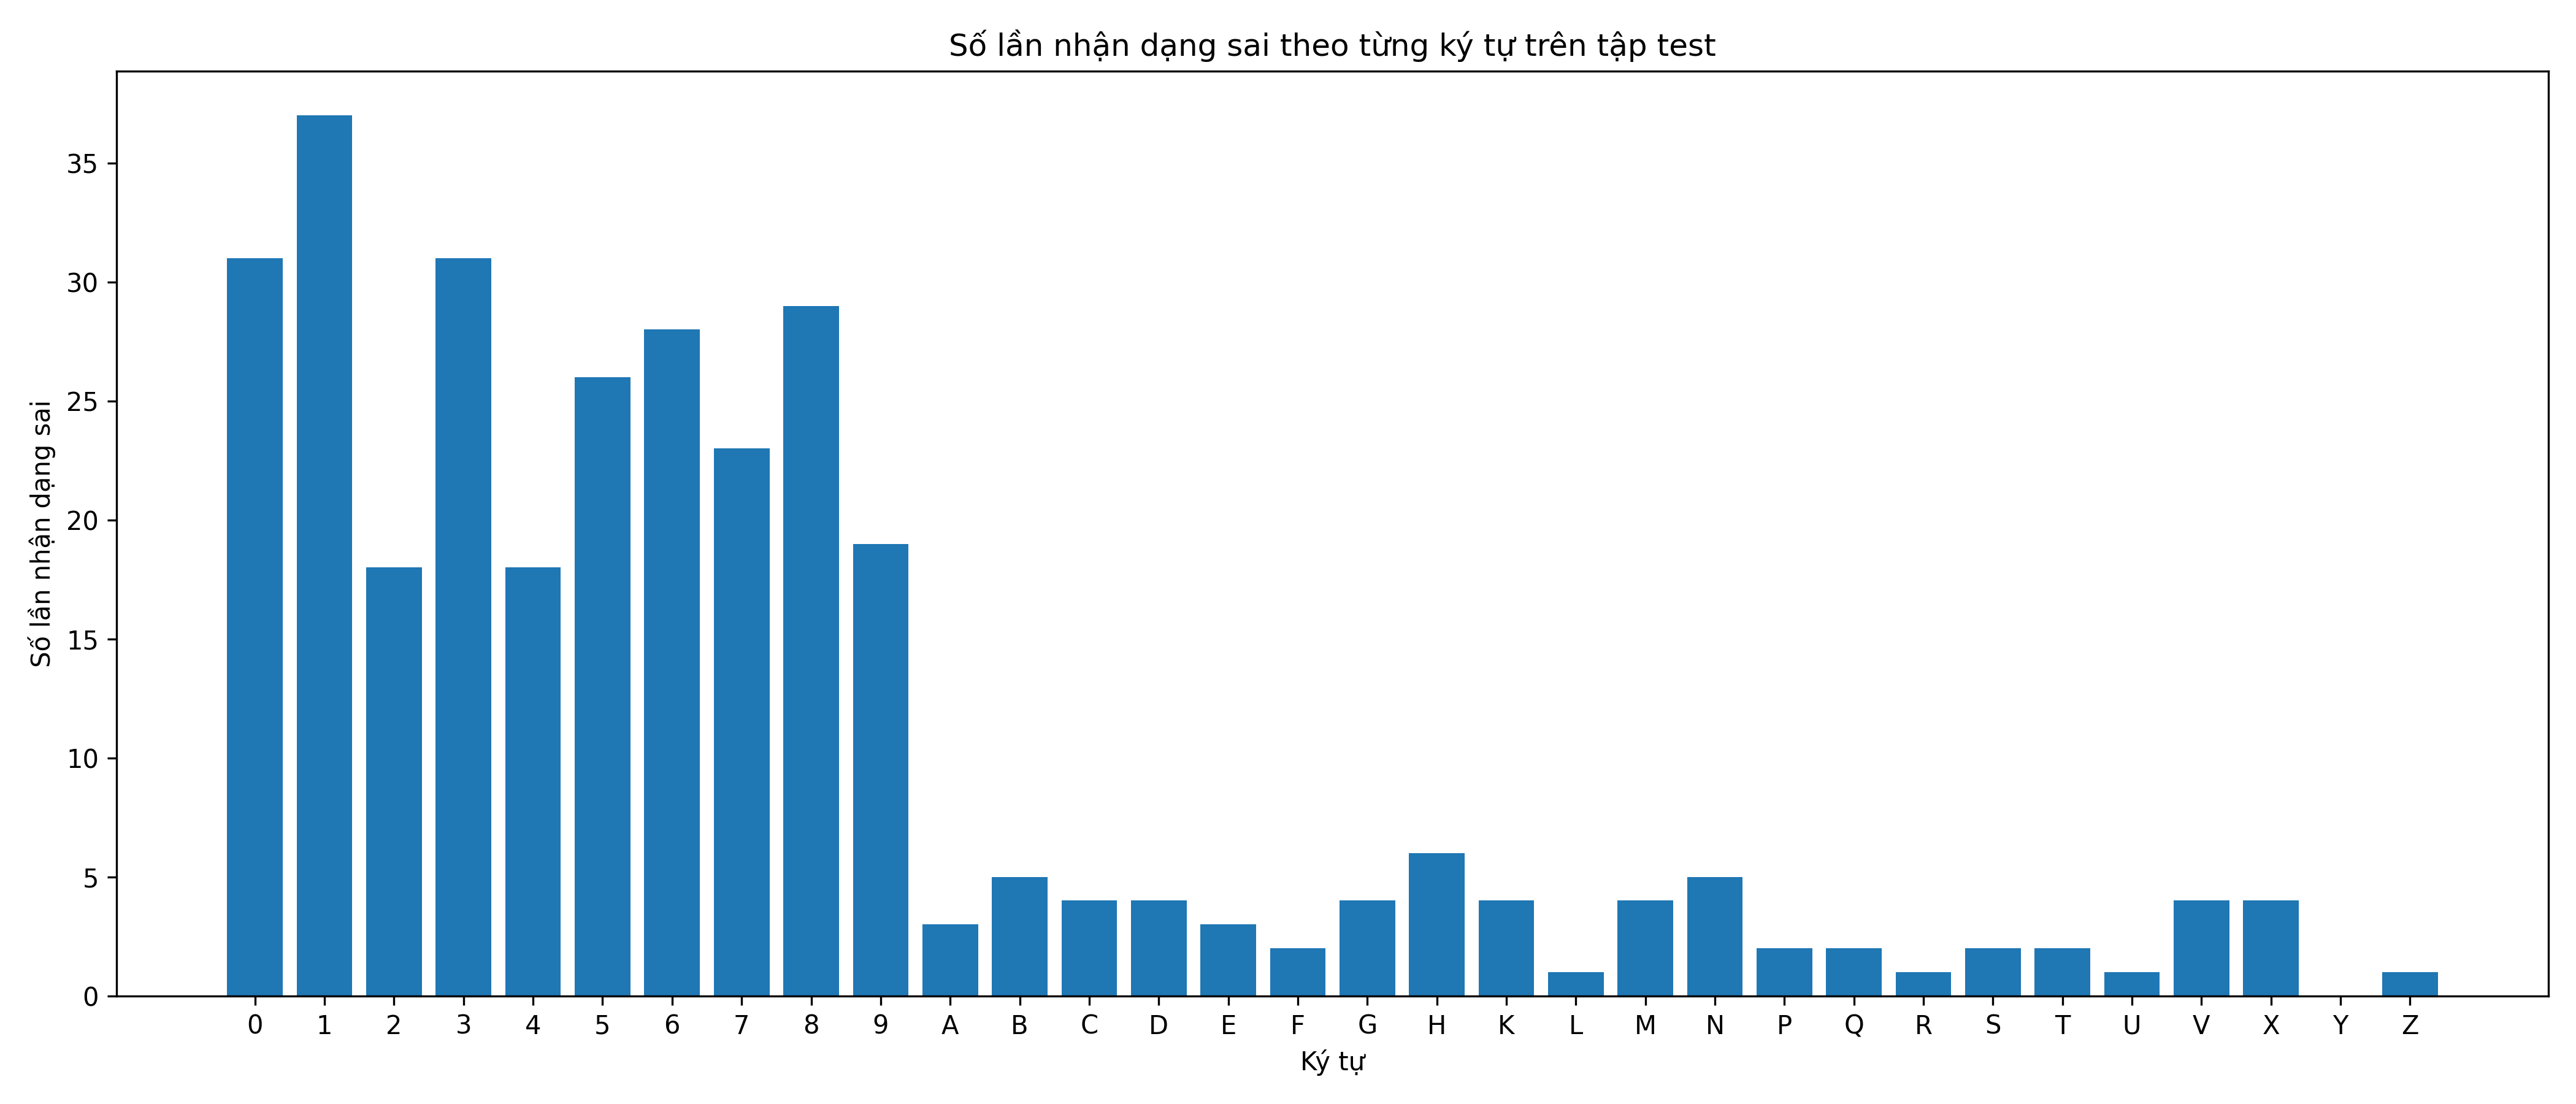
\includegraphics[width=1.0\textwidth]{images/ocr_wrong_char_count.png}
	\caption{Biểu đồ thống kê số lần nhận dạng sai theo từng ký tự trên tập test}
	\label{fig:ocr_wrong_char_count}
\end{figure}


\begin{figure}[H]
	\centering
	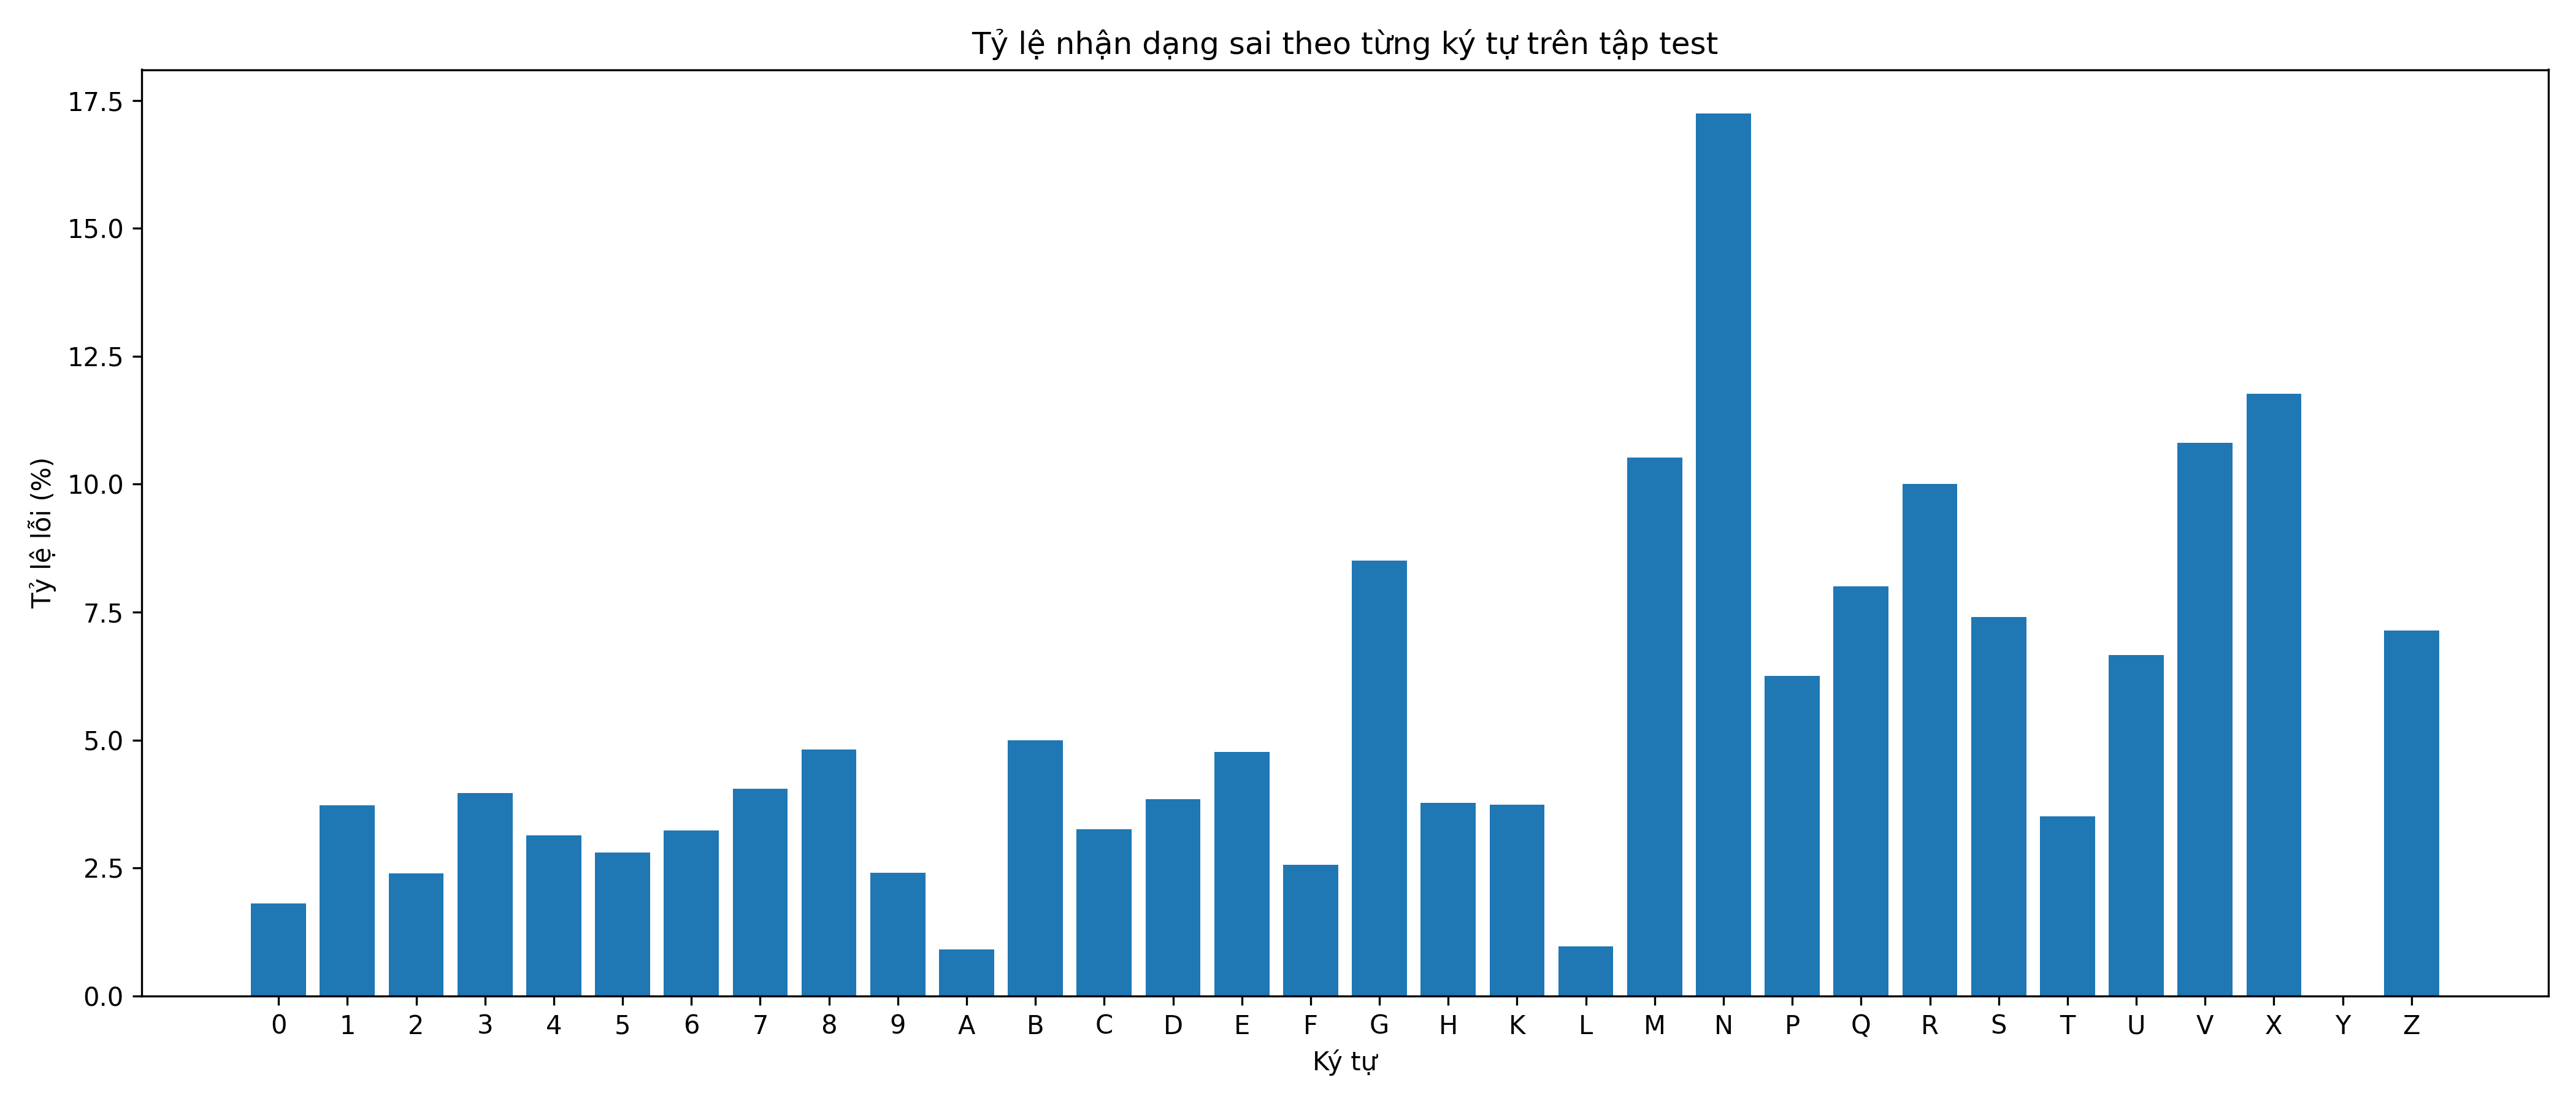
\includegraphics[width=1.0\textwidth]{images/ocr_char_error_rate.png}
	\caption{Biểu đồ thống kê tỉ lệ nhận dạng sai theo từng ký tự trên tập test}
	\label{fig:ocr_wrong_char_countu}
\end{figure}

Hình~\ref{fig:ocr_wrong_char_count} và Hình~\ref{fig:ocr_wrong_char_countu} phân tích 
lỗi nhận dạng ký tự trên tập test theo hai góc độ: số lần nhận dạng sai tuyệt 
đối và tỉ lệ lỗi tương đối. Về số lần sai, các chữ số \texttt{0}, \texttt{1}, 
\texttt{2}, \texttt{4}, \texttt{5}, \texttt{6}, \texttt{7}, \texttt{8} có tần 
suất lỗi cao nhất, điều này phần lớn phản ánh tần suất xuất hiện cao của chúng 
trong biển số xe hơn là độ khó nhận dạng thực sự. Khi xét tỉ lệ lỗi, bức 
tranh thay đổi rõ rệt: các chữ cái \texttt{N}, \texttt{P}, \texttt{Y}, 
\texttt{X}, \texttt{V} nổi bật với tỉ lệ nhận dạng sai cao, lên đến trên 
10\% đối với \texttt{N} và \texttt{P}. Đây là các ký tự xuất hiện ít trong 
tập huấn luyện nhưng có hình dạng dễ nhầm lẫn với các ký tự khác, dẫn đến 
hiệu suất nhận dạng thấp hơn đáng kể so với nhóm chữ số. Kết quả này cho 
thấy việc thu thập dữ liệu ký tự hiếm còn ít và việc tăng cường ảnh dữ liệu ký tự hiếm bằng phương pháp xoay ảnh và đổi không gian màu biển số chưa thực sự giải quyết đc vấn đề mất cần bằng dữ liệu.

\section{Demo ứng dụng}

\subsection{Quy trình hệ thống}

Sau khi hoàn thành huấn luyện mô hình phát hiện biển số và mô hình nhận dạng ký tự,  tiến hành tích hợp hai mô hình YOLOv8n và Paddle OCR vào hệ thống quản lý xe. Hệ thống được xây dựng nhằm hỗ trợ các thao tác cơ bản như nhận dạng biển số từ ảnh hoặc camera, lưu thông tin xe vào, xử lý xe ra, tính phí gửi xe và thống kê dữ liệu theo ngày.



\begin{figure}[H]
	\centering
	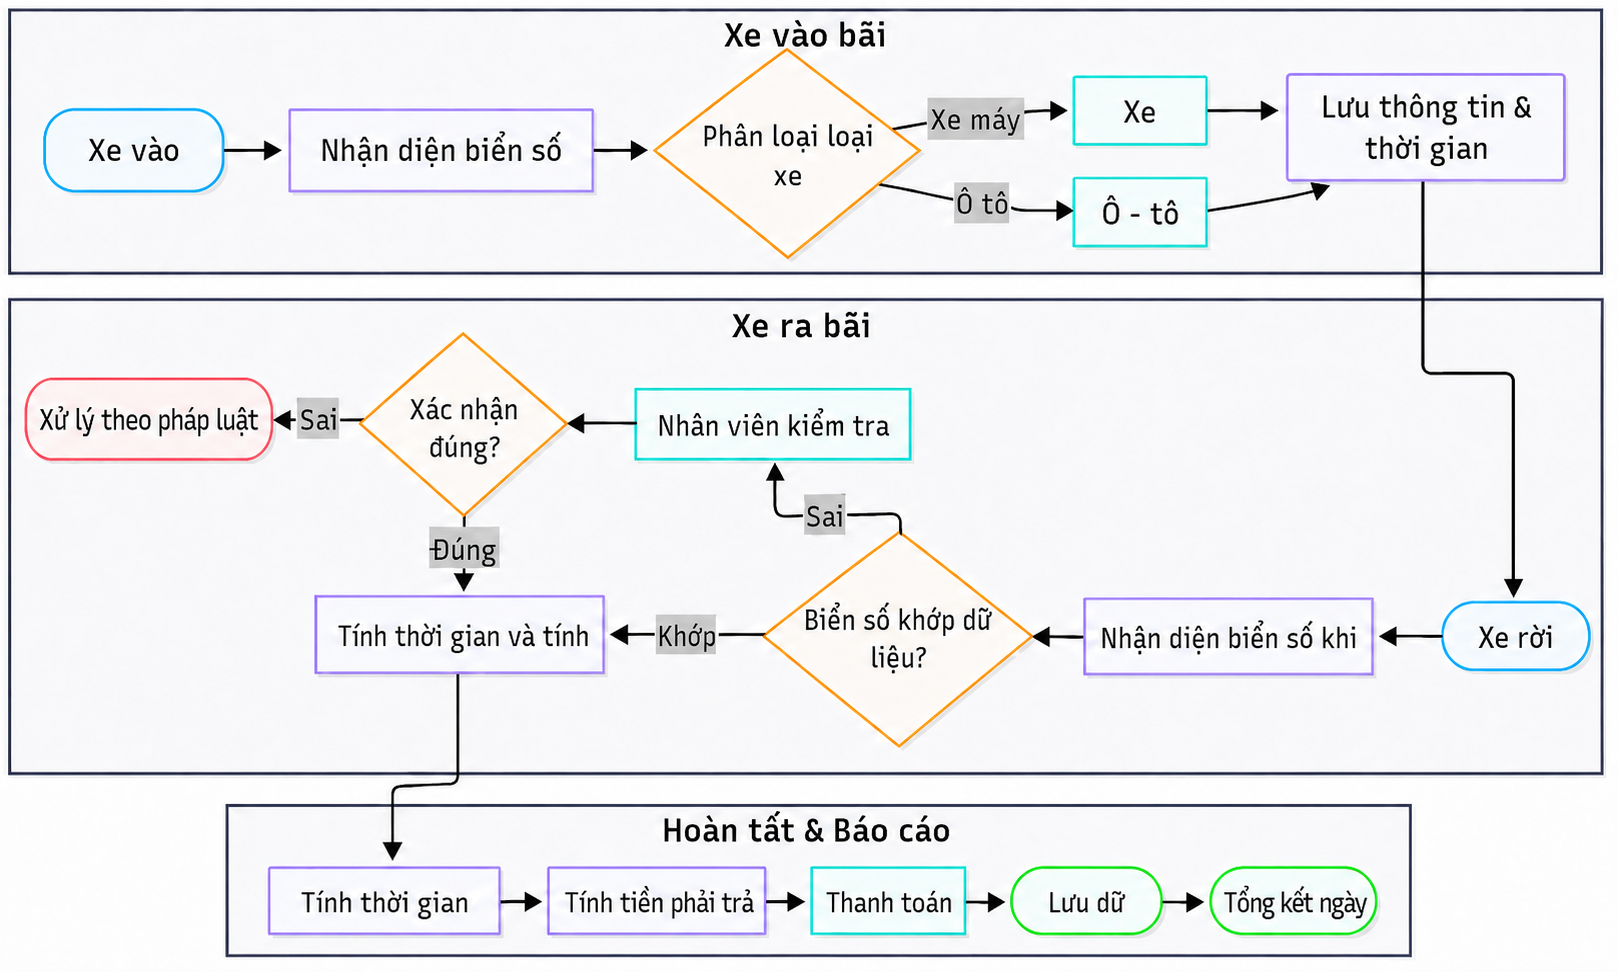
\includegraphics[width=1.0\textwidth]{images/system_pipeline.png}
	\caption{Quy trình nhận dạng biển số trong hệ thống quản lý xe ra vào}
	\label{fig:system_pipeline}
\end{figure}

Hệ thống trong sơ đồ mô tả quy trình quản lý xe vào và xe ra tại bãi giữ xe nhỏ. Quy trình được chia thành ba phần chính: xe vào bãi, xe ra bãi và hoàn tất báo cáo.

Ở phần xe vào bãi, khi phương tiện đi vào, hệ thống nhận diện biển số bằng mô hình đã huấn luyện. Sau đó, phương tiện được phân loại thành xe máy hoặc ô tô dự trên ký chữ cái trên biển số xe (ví dụ biển số 51G1-123.45 sẽ được phân loại là xe máy vì có ký tự G1). Kết quả nhận dạng biển số, loại xe và thời gian vào bãi được lưu lại để làm dữ liệu đối chiếu khi xe rời khỏi bãi.

Ở phần xe ra bãi, hệ thống tiếp tục nhận diện biển số của phương tiện khi rời bãi. Biển số vừa nhận dạng được so sánh với dữ liệu đã lưu trước đó. Nếu biển số khớp, hệ thống tính thời gian gửi xe và chuyển sang bước tính phí. Nếu biển số không khớp hoặc kết quả nhận dạng chưa chắc chắn, nhân viên sẽ kiểm tra lại. Trường hợp xác nhận đúng thì hệ thống tiếp tục xử lý thanh toán. Trường hợp sai hoặc có dấu hiệu bất thường thì chuyển sang bước xử lý theo pháp luật.

Ở phần hoàn tất và báo cáo, hệ thống tính thời gian gửi xe, tính số tiền phải trả, thực hiện thanh toán, lưu dữ liệu giao dịch và tổng kết ngày. Quy trình này giúp giảm thao tác ghi chép thủ công, hỗ trợ tra cứu xe vào ra, hạn chế nhầm lẫn biển số và cung cấp dữ liệu thống kê cho người quản lý bãi xe.

\subsection{Giao diện login}
\begin{figure}[H]
	\centering
	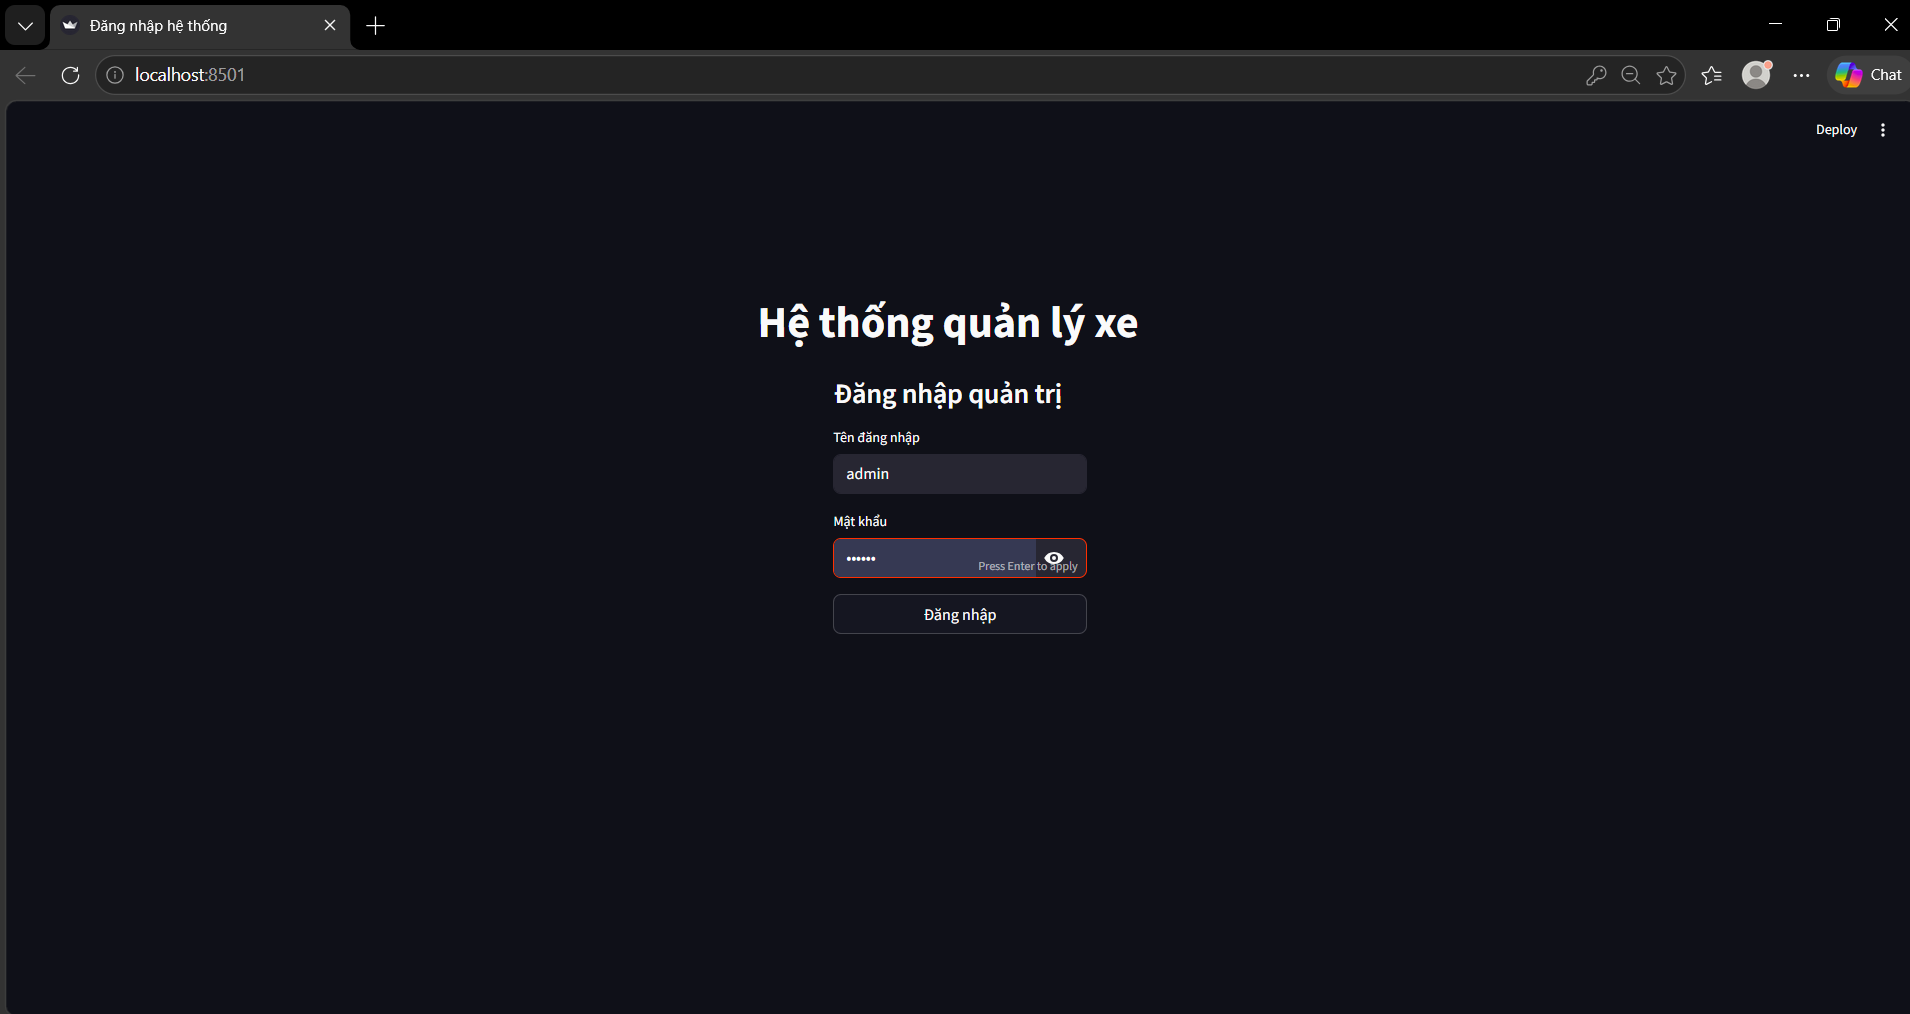
\includegraphics[width=1.0\textwidth]{images/gui_login.png}
	\caption{Giao diện đăng nhập}
	\label{fig:gui_login}
\end{figure}

Giao diện đăng nhập yêu cầu quản trị viên nhập tên đăng nhập và mật khẩu trước khi sử dụng hệ thống. Cách bố trí đơn giản, tập trung vào hai ô nhập liệu và nút đăng nhập, giúp giới hạn quyền truy cập vào các chức năng quản lý xe.

\subsection{giao diện chính hệ thống}

\begin{figure}[H]
	\centering
	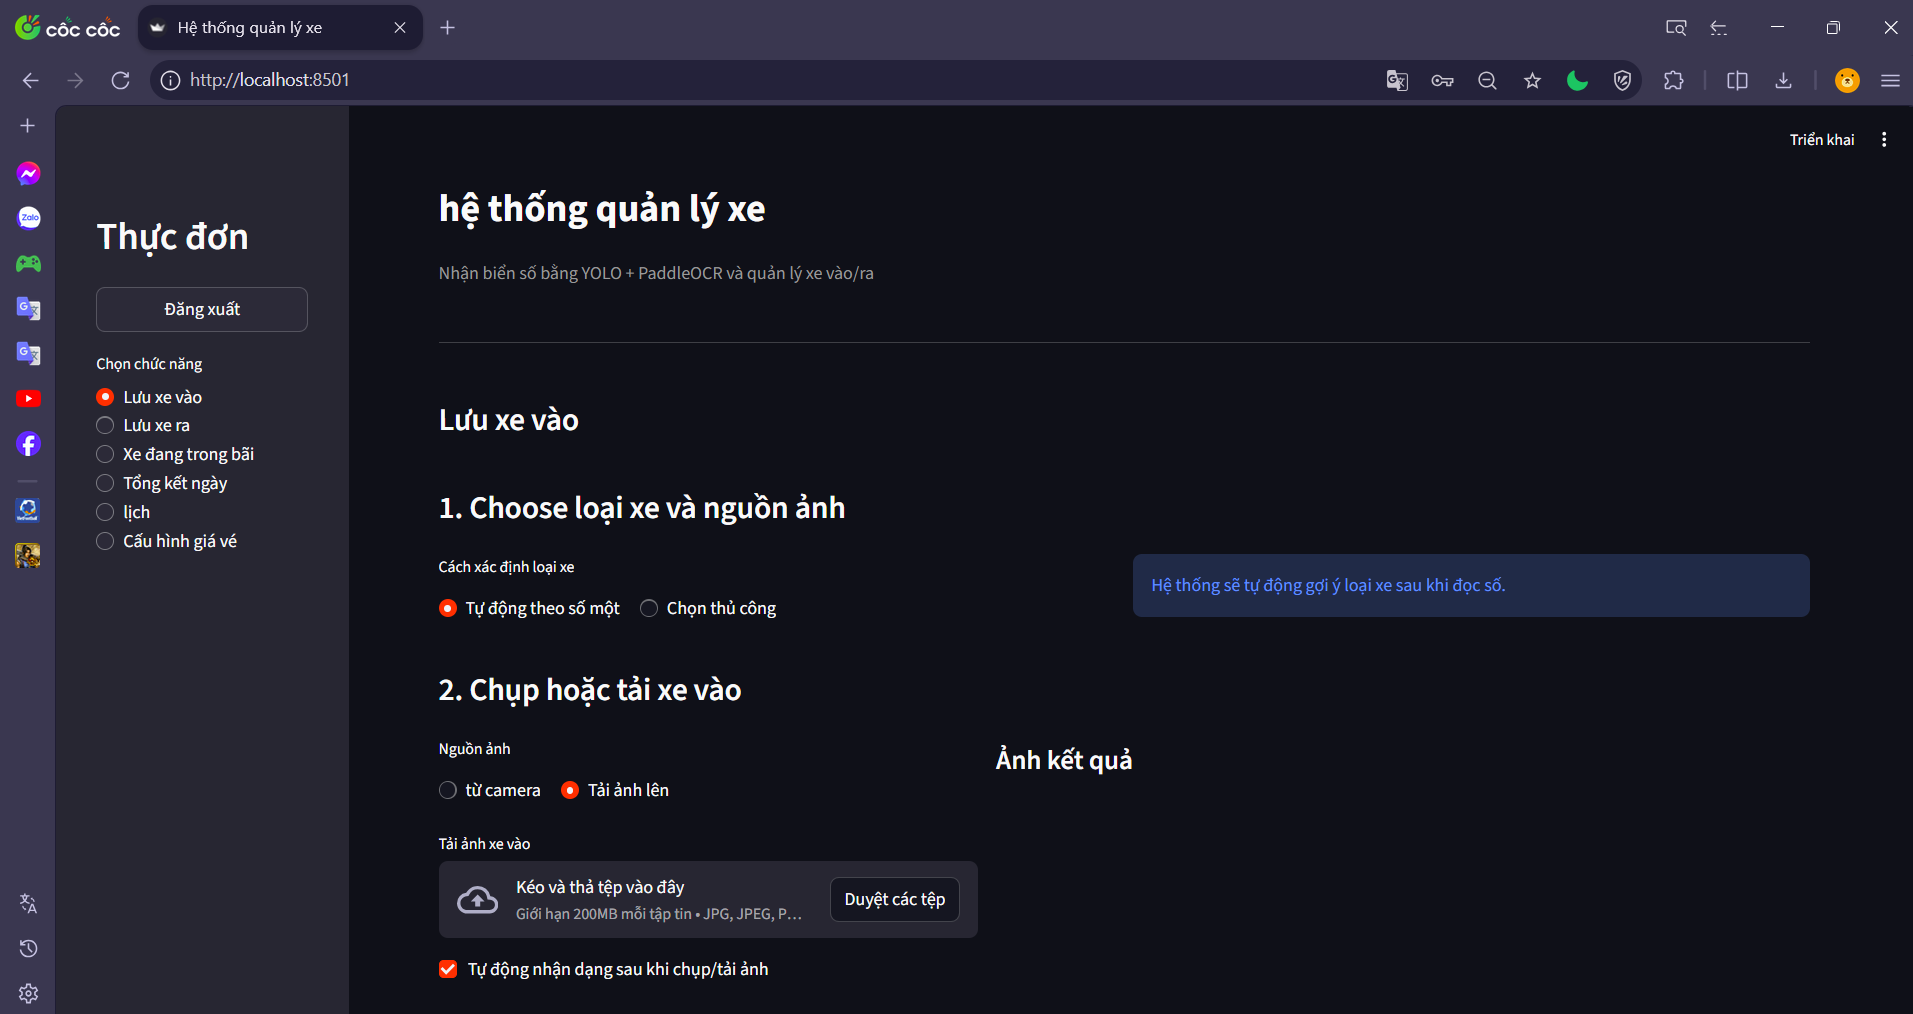
\includegraphics[width=1.0\textwidth]{images/gui_vehicle_in.png}
	\caption{Giao diện chính hệ thống}
	\label{fig:gui_vehicle_in}
\end{figure}

Giao diện lưu xe vào cho phép người dùng chọn cách xác định loại xe và nguồn ảnh đầu vào (1 người dùng tự chọn ô tô hay xe máy , 2 dựa vào ký tự biển số mà hệ thống đọc được, hệ thống sẽ đề xuất). Người dùng có thể chụp bằng camera hoặc tải ảnh lên. Sau khi nhận ảnh, hệ thống dùng YOLO để phát hiện biển số, dùng PaddleOCR để đọc ký tự và hiển thị kết quả nhận dạng trước khi lưu xe vào bãi.
\begin{figure}[H]
	\centering
	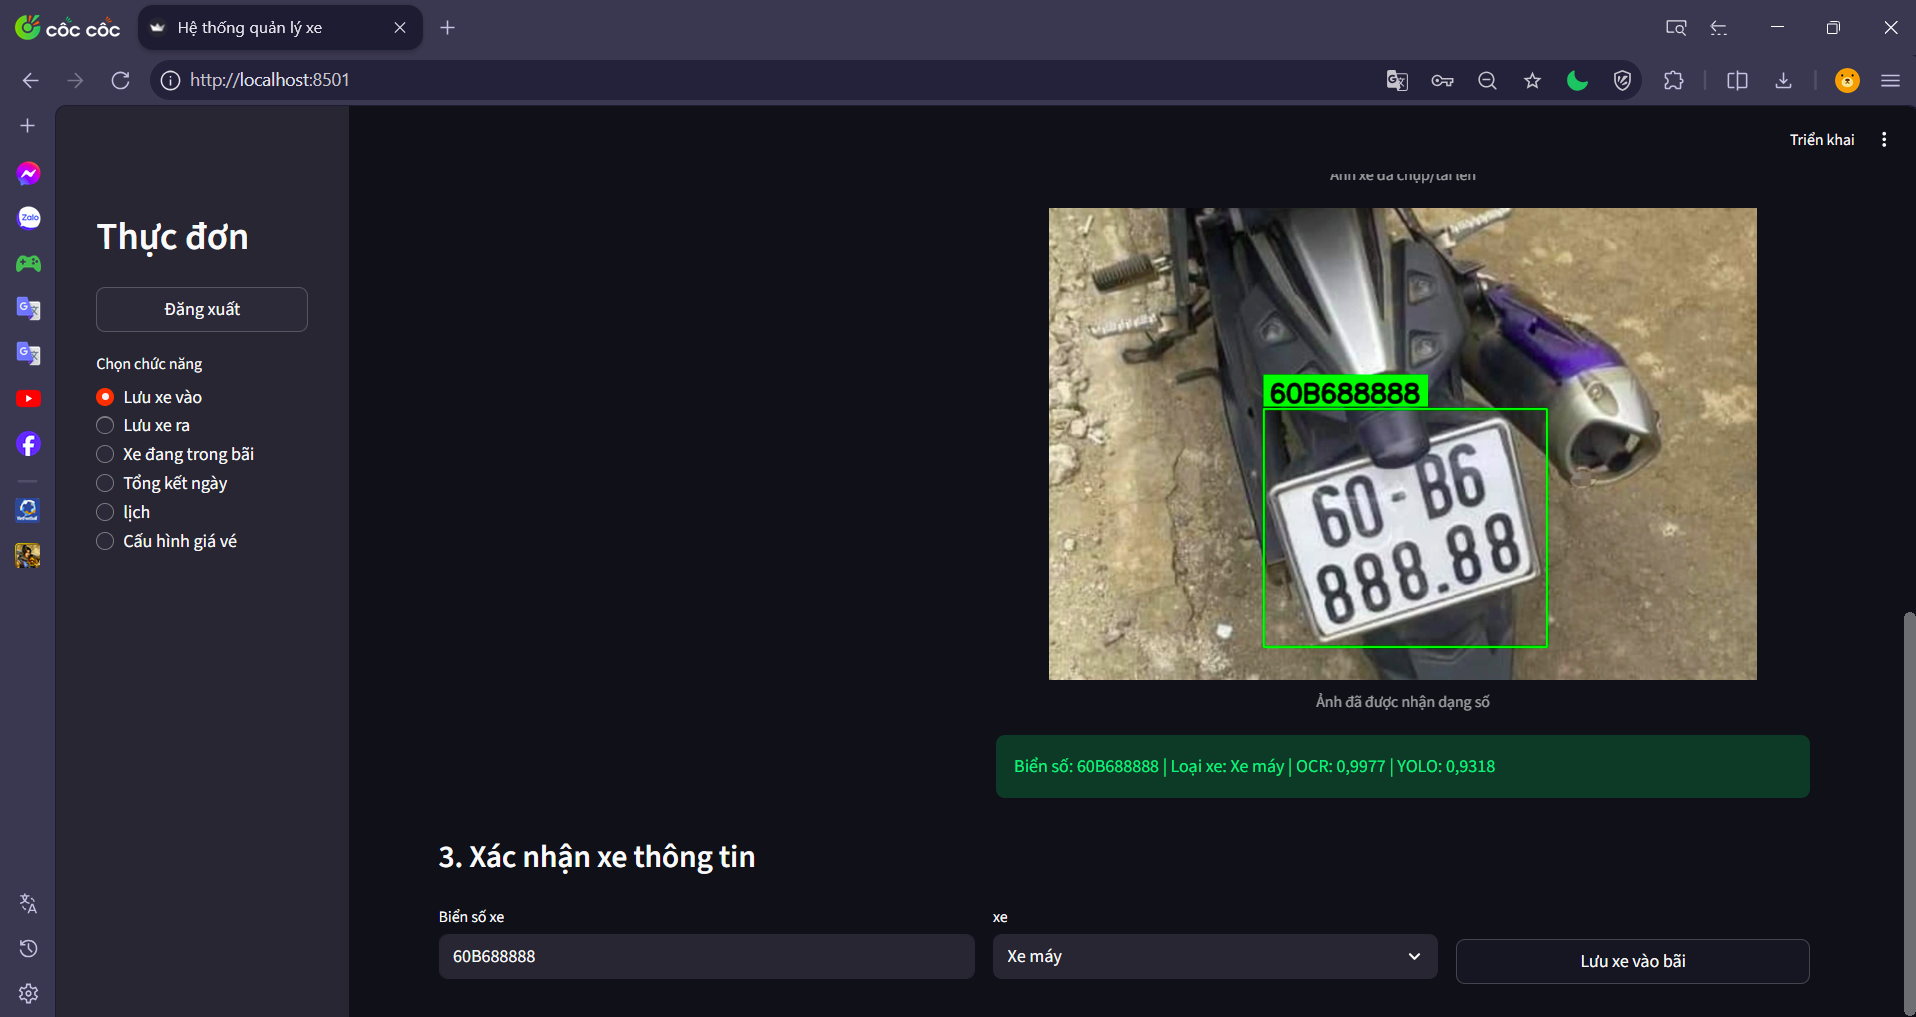
\includegraphics[width=1.0\textwidth]{images/xera.png}
	\caption{Giao diện chức năng lưu xe vào}
	\label{fig:gui_vehicle_in1}
\end{figure}
Giao diện này hiển thị ảnh xe sau khi đã phát hiện biển số. Hệ thống vẽ khung bao quanh biển số và hiển thị chuỗi ký tự OCR đọc được. Bên dưới có phần xác nhận thông tin gồm biển số, loại xe và nút lưu xe vào bãi. Người dùng vẫn có thể chỉnh lại biển số hoặc loại xe nếu kết quả nhận dạng chưa đúng.
\subsection{giao diện chức năng lưu xe ra}
\begin{figure}[H]
	\centering
	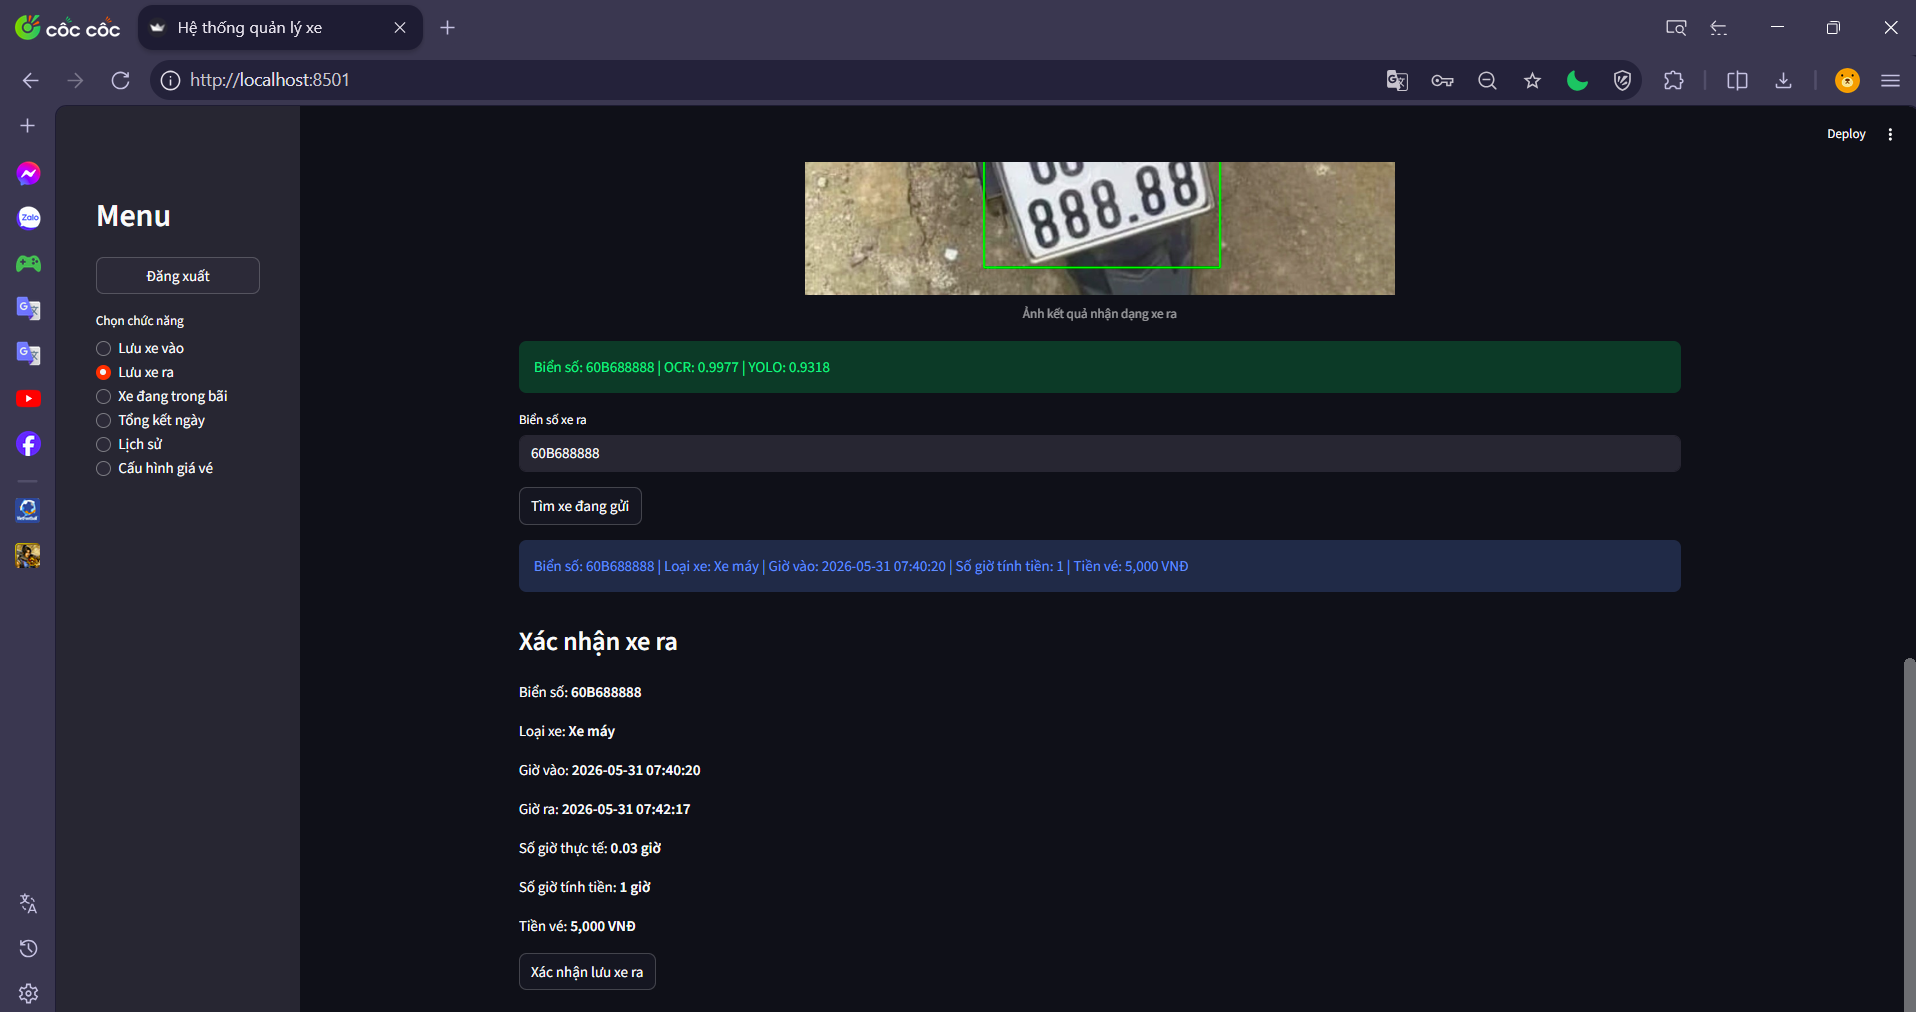
\includegraphics[width=1.0\textwidth]{images/gui_vehicle_out.png}
	\caption{Giao diện chức năng lưu xe ra}
	\label{fig:gui_vehicle_out}
\end{figure}

Giao diện lưu xe ra dùng để nhận dạng biển số khi phương tiện rời bãi. Sau khi ảnh được xử lý, hệ thống so sánh biển số với dữ liệu xe đang gửi. Nếu tìm thấy xe, hệ thống hiển thị giờ vào, giờ ra, số giờ tính tiền và tiền vé để nhân viên xác nhận lưu xe ra.



\subsection {những tính năng khác}
\begin{figure}[H]
	\centering
	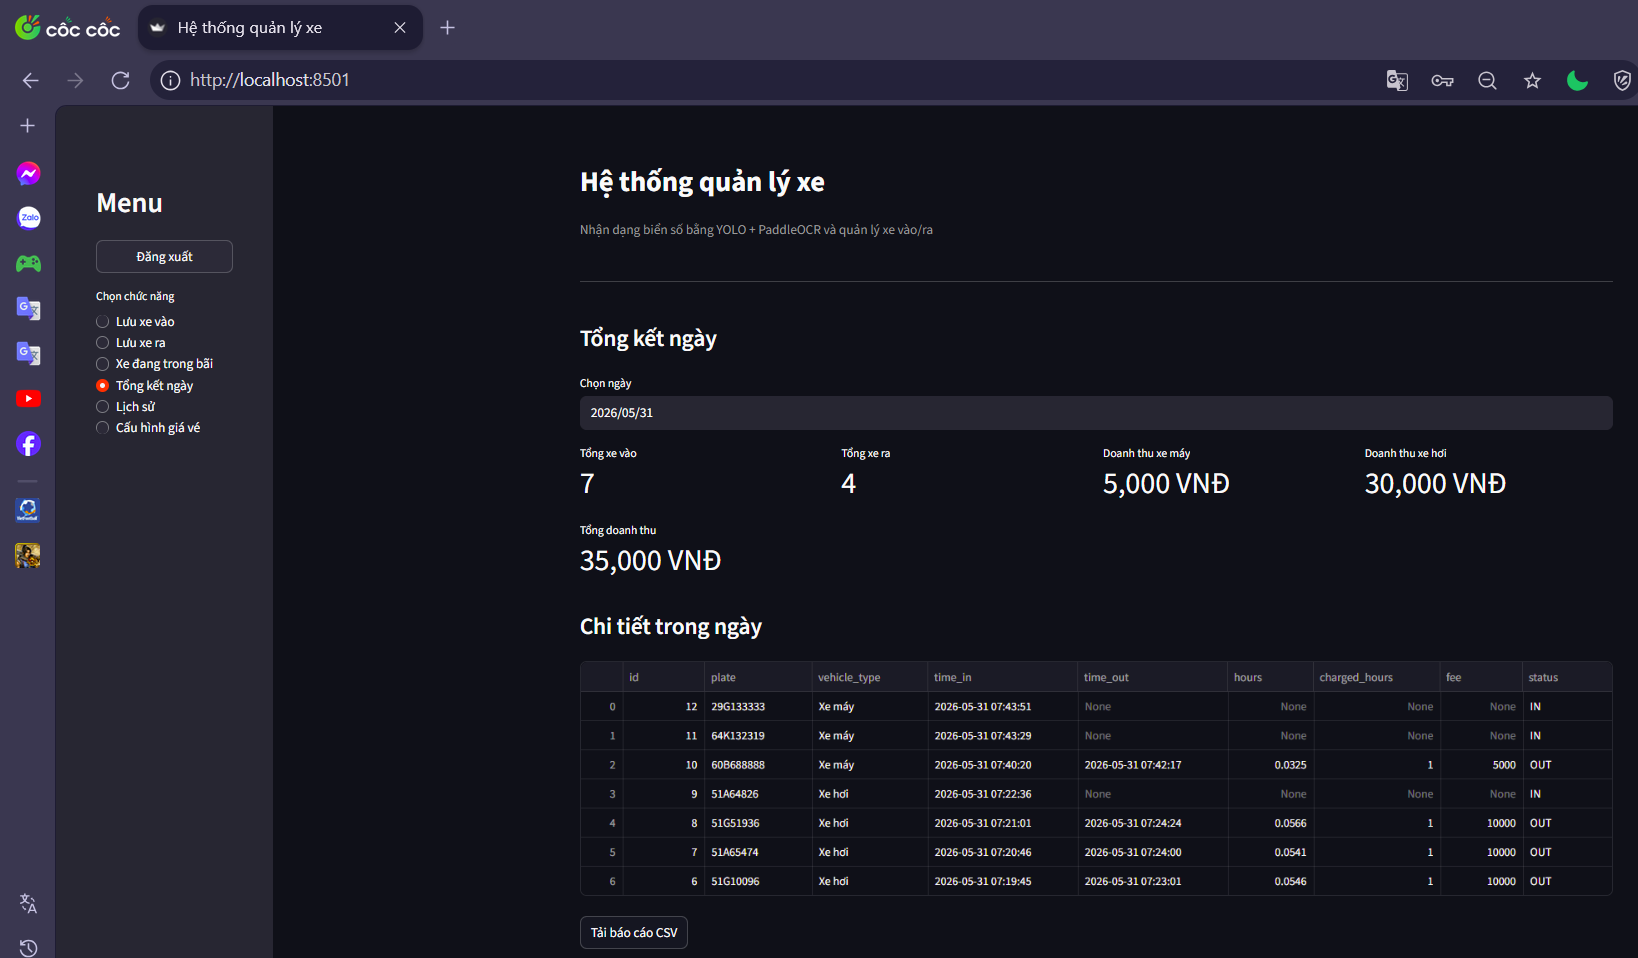
\includegraphics[width=1.0\textwidth]{images/gui_daily_summary.png}
	\caption{Giao diện tổng kết ngày}
	\label{fig:gui_daily_summary1}
\end{figure}
Giao diện tổng kết ngày hiển thị các chỉ số chính như tổng xe vào, tổng xe ra, doanh thu xe máy, doanh thu xe hơi và tổng doanh thu. Bên dưới là bảng chi tiết các lượt gửi xe trong ngày, gồm thời gian vào, thời gian ra, số giờ tính tiền, phí và trạng thái. Người dùng có thể in danh sách ra file .csv
\begin{figure}[H]
	\centering
	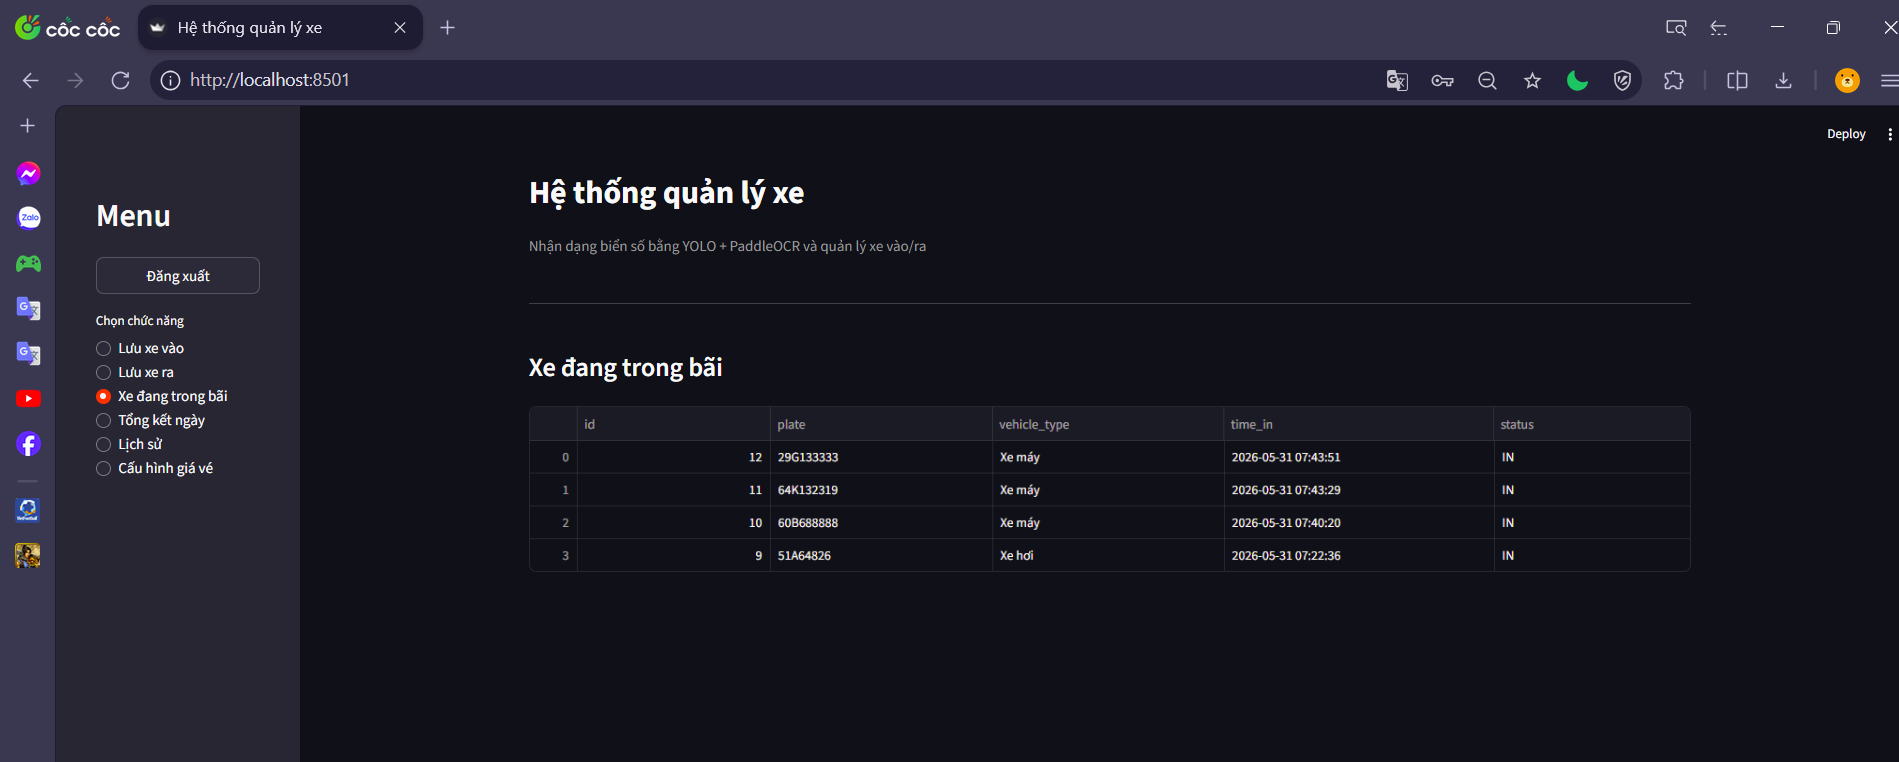
\includegraphics[width=1.0\textwidth]{images/thongke.png}
	\caption{Giao diện lịch sử trong ngày }
	\label{fig:gui_daily_summary2}
\end{figure}
Giao diện lịch sử lưu lại toàn bộ các lượt xe vào và xe ra. Bảng dữ liệu giúp người dùng tra cứu lại biển số, loại xe, thời gian gửi, phí thanh toán và trạng thái của từng bản ghi.

\begin{figure}[H]
	\centering
	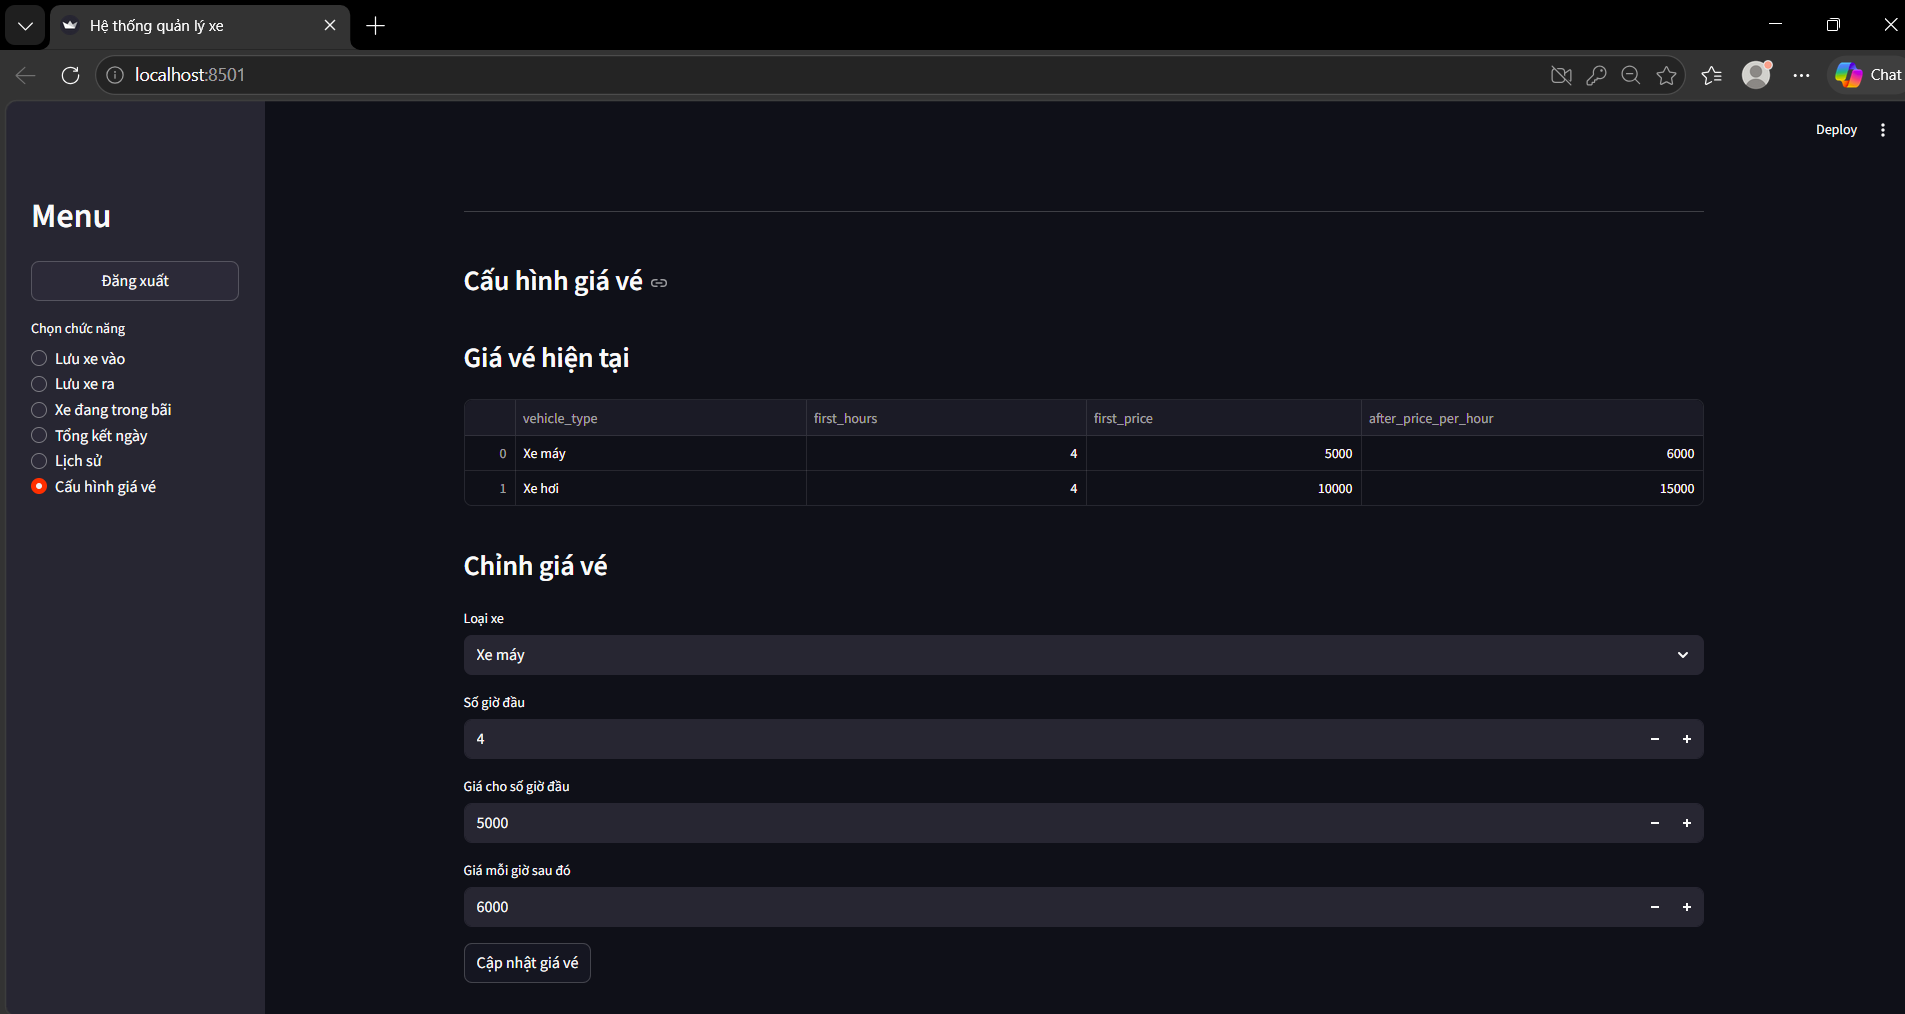
\includegraphics[width=1.0\textwidth]{images/chinhgia.png}
	\caption{Giao diện cấu hình giá vé }
	\label{fig:gui_daily_summary3}
\end{figure}
Giao diện cấu hình giá vé cho phép quản trị viên xem và chỉnh giá gửi xe cho từng loại phương tiện. Hệ thống hỗ trợ thiết lập số giờ đầu, giá cho số giờ đầu và giá mỗi giờ sau đó. Các thông tin này được dùng trực tiếp khi tính phí xe ra.

% =====================================================
\chapter{KẾT LUẬN VÀ KIẾN NGHỊ}
% =====================================================

\section{Kết quả đạt được}

Đề tài đã xây dựng được hệ thống nhận dạng biển số xe và quản lý xe ra vào ở mức thử nghiệm. Hệ thống gồm hai thành phần chính: mô hình YOLO dùng để phát hiện vùng biển số và mô hình PaddleOCR dùng để nhận dạng chuỗi ký tự trên ảnh biển số đã được cắt ra. Kết quả nhận dạng được đưa vào ứng dụng quản lý xe, hỗ trợ các chức năng lưu xe vào, lưu xe ra, tính phí gửi xe, thống kê xe đang trong bãi, tổng kết ngày và cấu hình giá vé.

Về dữ liệu phát hiện biển số, đề tài đã tổ chức bộ dữ liệu YOLO gồm 4.578 ảnh có nhãn. Trong đó, tập train có 3.633 ảnh, tập validation có 472 ảnh và tập test có 473 ảnh. Phần lớn ảnh trong bộ dữ liệu chứa một biển số, chiếm 90,80\% toàn bộ dữ liệu. Ngoài ra, dữ liệu vẫn có 271 ảnh chứa hai biển số và 150 ảnh chứa trên hai biển số. Điều này giúp mô hình học được cả trường hợp phổ biến và một số tình huống có nhiều biển số trong cùng một ảnh.

Mô hình YOLOv8n đã được huấn luyện để phát hiện vùng biển số. Sau khi kiểm tra lại trên tập test gồm 473 ảnh và 553 đối tượng biển số, mô hình đạt Precision 0,9558, Recall 0,8608, mAP50 0,8610 và mAP50-95 0,7689. Kết quả này cho thấy mô hình có khả năng phát hiện biển số tương đối tốt, đặc biệt là tỷ lệ dự đoán đúng trong các vùng được phát hiện khá cao. Tuy vậy, Recall thấp hơn Precision cho thấy mô hình vẫn còn bỏ sót một số biển số trong điều kiện ảnh khó.

Đối với mô hình OCR, đề tài đã chuẩn bị dữ liệu nhận dạng ký tự biển số, làm sạch nhãn, bổ sung ký tự hiếm và cân bằng lại tập train bằng các kỹ thuật tăng cường ảnh. Mô hình PaddleOCR được huấn luyện trên ảnh biển số đã chuẩn hóa về kích thước phù hợp. Trong quá trình huấn luyện, Accuracy trên tập train tăng từ 0,0000 ở epoch đầu lên 0,9453 ở epoch 50. Norm Edit Distance tăng từ 0,1878 lên 0,9891, trong khi CTC Loss giảm từ 81,3232 xuống 0,2902. Kết quả tốt nhất trên validation đạt Accuracy 0,8555 và Norm Edit Distance 0,9599. Các chỉ số này cho thấy mô hình đã học được đặc trưng ký tự biển số sau quá trình xử lý và cân bằng dữ liệu.

Đề tài cũng đã thực hiện phân tích lỗi nhận dạng ký tự trên tập test. Kết quả cho thấy các chữ số xuất hiện nhiều nên có số lần sai tuyệt đối cao, chẳng hạn ký tự 3 sai 39 lần, ký tự 1 sai 33 lần, ký tự 8 sai 38 lần và ký tự . Khi xét theo tỷ lệ lỗi, một số ký tự hiếm có tỷ lệ sai cao hơn, N sai 18,18\%, M sai 11,00\% và X sai 12,29\%. Kết quả này phản ánh đúng đặc điểm của bài toán OCR biển số, trong đó các ký tự ít xuất hiện thường khó học ổn định hơn các ký tự phổ biến.

Về mặt ứng dụng, hệ thống demo đã tích hợp được quy trình nhận dạng vào giao diện Streamlit. Khi người dùng chụp hoặc tải ảnh xe, hệ thống phát hiện vùng biển số bằng YOLO, cắt ảnh biển số, đưa ảnh crop vào PaddleOCR và trả về chuỗi biển số. Người dùng có thể kiểm tra kết quả, chỉnh sửa thủ công nếu cần, sau đó lưu thông tin xe vào cơ sở dữ liệu SQLite. Khi xe ra, hệ thống nhận dạng lại biển số, đối chiếu với dữ liệu đang gửi, tính thời gian gửi xe và tính phí theo cấu hình giá vé. Giao diện cũng hỗ trợ xem danh sách xe đang trong bãi, lịch sử gửi xe, tổng kết ngày và chỉnh giá vé.

Nhìn chung, đề tài đã hoàn thành được mục tiêu xây dựng một hệ thống thử nghiệm cho bài toán nhận dạng biển số và quản lý xe ra vào. Hệ thống đã kết nối được các bước từ phát hiện biển số, nhận dạng ký tự đến lưu trữ và xử lý nghiệp vụ. Các kết quả thực nghiệm cho thấy mô hình có khả năng hoạt động trên dữ liệu đã chuẩn bị, đồng thời chỉ ra rõ các lỗi còn tồn tại để tiếp tục cải thiện.

\section{Hạn chế của đề tài}

Mặc dù hệ thống đã hoạt động được ở mức thử nghiệm, đề tài vẫn còn một số hạn chế. Hạn chế đầu tiên nằm ở chất lượng và độ đa dạng của dữ liệu. Dữ liệu biển số được thu thập từ nhiều nguồn nhưng vẫn chưa bao phủ đầy đủ các điều kiện thực tế như ánh sáng yếu, biển số phản sáng,ảnh không rõ, biển số bị che khuất,góc chụp lệch mạnh . Những điều kiện này làm giảm chất lượng phát hiện của YOLO và làm OCR nhận dạng sai ký tự.

Hạn chế thứ hai là dữ liệu OCR vẫn còn mất cân bằng giữa các ký tự. Các chữ số xuất hiện nhiều hơn chữ cái, trong khi một số ký tự hiếm như R, U, Y, Z, N hoặc M có số lượng mẫu thấp hơn. Mặc dù đề tài đã bổ sung ký tự hiếm và dùng tăng cường dữ liệu, kết quả phân tích lỗi cho thấy một số ký tự hiếm vẫn có tỷ lệ sai cao. Điều này cho thấy tăng cường ảnh có tác dụng hỗ trợ nhưng chưa thay thế được dữ liệu thực tế đa dạng. Nếu số ảnh gốc của một ký tự còn ít, việc tạo thêm biến thể từ cùng một nhóm ảnh vẫn chưa đủ để mô hình học ổn định.

Hạn chế thứ ba nằm ở sự khác biệt giữa tập test OCR và ảnh chạy trên giao diện thực tế. Khi kiểm tra mô hình OCR trên tập test, ảnh đầu vào thường là ảnh biển số đã được crop và chuẩn hóa. Trong giao diện hệ thống, ảnh OCR lại được lấy từ kết quả crop của YOLO trên ảnh xe gốc. Nếu YOLO crop lệch, crop quá sát, ảnh bị mờ hoặc biển số nhỏ, PaddleOCR có thể đọc sai, dù mô hình đạt kết quả tốt trên tập test. Đây là một điểm hạn chế thường gặp khi ghép nhiều mô hình thành một pipeline hoàn chỉnh.

Hạn chế thứ tư là việc phân loại xe máy và xe hơi trong hệ thống vẫn mang tính gợi ý. Hệ thống hiện dựa vào chuỗi biển số để suy đoán loại xe, nhưng cách này không đủ chắc chắn vì biển số Việt Nam có nhiều trường hợp ngoại lệ. Do đó, giao diện vẫn cần cho phép người dùng chọn hoặc chỉnh lại loại xe trước khi lưu. Nếu triển khai trong thực tế, nên dùng thêm mô hình phân loại phương tiện dựa trên ảnh hoặc dữ liệu đăng ký xe thay vì chỉ dựa vào chuỗi biển số.

Hạn chế thứ năm là hệ thống quản lý mới dừng ở mức demo. Cơ sở dữ liệu SQLite phù hợp cho thử nghiệm nhỏ, nhưng chưa phù hợp với môi trường nhiều máy, nhiều camera hoặc nhiều người dùng truy cập đồng thời. Phần đăng nhập quản trị còn đơn giản, mật khẩu được khai báo trực tiếp trong code nên chưa đáp ứng yêu cầu bảo mật. Hệ thống cũng chưa có chức năng phân quyền, sao lưu dữ liệu, đồng bộ với thiết bị cổng ra vào hoặc xử lý video thời gian thực.

Ngoài ra, hệ thống vẫn cần kiểm tra thủ công trong một số tình huống. Khi mô hình nhận dạng sai biển số hoặc bỏ sót ký tự, nhân viên phải chỉnh lại trước khi lưu. Điều này là phù hợp với một hệ thống thử nghiệm, nhưng nếu muốn vận hành ổn định trong môi trường thực tế thì cần cải thiện độ chính xác và bổ sung cơ chế cảnh báo các trường hợp có độ tin cậy thấp.

\section{Hướng phát triển}

Trong thời gian tới, hướng phát triển đầu tiên là tiếp tục mở rộng và cải thiện dữ liệu. Cần thu thập thêm ảnh biển số thực tế trong nhiều điều kiện khác nhau, đặc biệt là ảnh thiếu sáng, ảnh bị rung, ảnh biển số nghiêng, biển số xe máy hai dòng và đặc biệt là biển số có ký tự hiếm. Việc bổ sung dữ liệu thật có ý nghĩa lớn hơn so với chỉ tăng cường ảnh từ một số mẫu gốc ít ỏi. Dữ liệu mới nên được kiểm tra nhãn cẩn thận để tránh mô hình học sai từ nhãn không chính xác.

Hướng phát triển thứ hai là cải thiện pipeline giữa YOLO và OCR. Thay vì đưa trực tiếp ảnh crop từ YOLO vào PaddleOCR, hệ thống có thể bổ sung bước căn chỉnh biển số, loại bỏ nền thừa, tăng tương phản và chuẩn hóa ảnh crop theo đúng định dạng của dữ liệu huấn luyện OCR. Với biển số nghiêng hoặc biển số hai dòng, có thể nghiên cứu thêm phương pháp hiệu chỉnh phối cảnh hoặc tách dòng ký tự trước khi nhận dạng. Điều này giúp giảm sự khác biệt giữa ảnh trong tập train và ảnh khi chạy thực tế trên giao diện.

Hướng phát triển thứ ba là cải thiện mô hình OCR. Có thể tiếp tục huấn luyện với dữ liệu cân bằng hơn, thử các cấu hình nhận dạng khác trong PaddleOCR hoặc so sánh thêm với các mô hình OCR khác. Ngoài Accuracy, cần theo dõi thêm tỷ lệ lỗi theo từng ký tự, tỷ lệ sai theo từng loại biển số và các cặp ký tự dễ nhầm. Những phân tích này giúp điều chỉnh dữ liệu đúng trọng tâm thay vì tăng dữ liệu một cách chung chung.

Hướng phát triển thứ tư là bổ sung mô hình phân loại phương tiện. Thay vì suy đoán xe máy hoặc xe hơi từ chuỗi biển số, hệ thống có thể dùng một mô hình phân loại ảnh để nhận biết loại phương tiện. Mô hình này nhận ảnh xe đầu vào và trả về nhãn xe máy hoặc xe hơi. Khi kết hợp với OCR, hệ thống sẽ xác định loại xe chính xác hơn và giảm thao tác chỉnh sửa của người dùng.

Hướng phát triển thứ năm là nâng cấp hệ thống quản lý. Cơ sở dữ liệu có thể chuyển từ SQLite sang MySQL, PostgreSQL hoặc một hệ quản trị cơ sở dữ liệu phù hợp hơn nếu cần triển khai cho nhiều người dùng. Hệ thống cũng nên bổ sung phân quyền tài khoản, mã hóa mật khẩu, sao lưu dữ liệu, tìm kiếm lịch sử theo biển số, xuất báo cáo theo ngày hoặc tháng và quản lý nhiều làn xe vào ra.

Hướng phát triển cuối cùng là triển khai hệ thống với camera thật. Khi đó, hệ thống cần xử lý luồng video, chọn khung hình rõ nhất, tránh nhận dạng lặp lại nhiều lần cho cùng một xe và tối ưu tốc độ suy luận. Đồng thời, cần thiết kế cơ chế xác nhận trong trường hợp mô hình có độ tin cậy thấp. Cách tiếp cận này giúp hệ thống tiến gần hơn đến ứng dụng thực tế, nhưng vẫn giữ vai trò kiểm tra của con người đối với các tình huống khó hoặc nhạy cảm.


\begin{thebibliography}{99}
	
	\bibitem{redmon2016yolo}
	Redmon, J., Divvala, S., Girshick, R., and Farhadi, A. (2016). You Only Look Once: Unified, Real-Time Object Detection. Proceedings of the IEEE Conference on Computer Vision and Pattern Recognition, 779--788. \url{https://arxiv.org/abs/1506.02640}
	
	\bibitem{bochkovskiy2020yolov4}
	Bochkovskiy, A., Wang, C.-Y., and Liao, H.-Y.M. (2020). YOLOv4: Optimal Speed and Accuracy of Object Detection. arXiv preprint arXiv:2004.10934. \url{https://arxiv.org/abs/2004.10934}
	
	\bibitem{ultralytics_yolov8}
	Ultralytics. (2023). YOLOv8 Documentation. \url{https://docs.ultralytics.com/models/yolov8/}
	
	\bibitem{du2020ppocr}
	Du, Y., Li, C., Guo, R., Yin, X., Liu, W., Zhou, J., Bai, Y., Yu, Z., Yang, Y., Dang, Q., and Wang, H. (2020). PP-OCR: A Practical Ultra Lightweight OCR System. arXiv preprint arXiv:2009.09941. \url{https://arxiv.org/abs/2009.09941}
	
	\bibitem{li2022ppocrv3}
	Li, C., Liu, W., Guo, R., Yin, X., Jiang, K., Du, Y., Du, Y., Zhu, L., Lai, B., Hu, X., Yu, D., and Ma, Y. (2022). PP-OCRv3: More Attempts for the Improvement of Ultra Lightweight OCR System. arXiv preprint arXiv:2206.03001. \url{https://arxiv.org/abs/2206.03001}
	
	\bibitem{paddleocr_docs}
	PaddlePaddle. (2026). PaddleOCR Documentation. \url{https://paddlepaddle.github.io/PaddleOCR/main/en/index.html}
	
	\bibitem{paddleocr_github}
	PaddlePaddle. (2026). PaddleOCR GitHub Repository. \url{https://github.com/PaddlePaddle/PaddleOCR}
	
	\bibitem{graves2006ctc}
	Graves, A., Fernandez, S., Gomez, F., and Schmidhuber, J. (2006). Connectionist Temporal Classification: Labelling Unsegmented Sequence Data with Recurrent Neural Networks. Proceedings of the 23rd International Conference on Machine Learning, 369--376. \url{https://www.cs.toronto.edu/~graves/icml_2006.pdf}
	
	\bibitem{levenshtein1966}
	Levenshtein, V.I. (1966). Binary Codes Capable of Correcting Deletions, Insertions and Reversals. Soviet Physics Doklady, 10(8), 707--710. \url{https://nymity.ch/sybilhunting/pdf/Levenshtein1966a.pdf}
	
	\bibitem{liao2019dbnet}
	Liao, M., Wan, Z., Yao, C., Chen, K., and Bai, X. (2019). Real-time Scene Text Detection with Differentiable Binarization. arXiv preprint arXiv:1911.08947. \url{https://arxiv.org/abs/1911.08947}
	
	\bibitem{opencv_docs}
	OpenCV. (2026). OpenCV Documentation. \url{https://docs.opencv.org/4.x/}
	
	\bibitem{streamlit_docs}
	Streamlit. (2026). Streamlit Documentation. \url{https://docs.streamlit.io/}
	
	\bibitem{sqlite_docs}
	SQLite. (2026). SQLite Documentation. \url{https://sqlite.org/docs.html}
	
	\bibitem{python_sqlite3}
	Python Software Foundation. (2026). sqlite3 DB-API 2.0 Interface for SQLite Databases. \url{https://docs.python.org/3/library/sqlite3.html}
	
	\bibitem{matplotlib_docs}
	Matplotlib Development Team. (2026). Matplotlib Documentation. \url{https://matplotlib.org/stable/index.html}
	
	\bibitem{kaggle_yolo_licenseplates}
	Nguyen, D.D. (2024). Licenseplates. Kaggle Dataset. \url{https://www.kaggle.com/datasets/duydieunguyen/licenseplates}
	
	\bibitem{kaggle_vietnamese_plate_ocr}
	topkek69. (2024). Vietnamese License Plate OCR. Kaggle Dataset. \url{https://www.kaggle.com/datasets/topkek69/vietnamese-license-plate-ocr}
\end{thebibliography}

\end{document}